\documentclass[11pt,a4paper]{book}

%------- packges ---------_%
% author's contact footnote
\usepackage{authblk}
\usepackage[right=1.25in,left=1.25in,top=1.1in,bottom=1.1in]{geometry}
% math tools
\usepackage{amsmath}
\usepackage{amsfonts}
\usepackage{amssymb}
\usepackage{amsthm}
\usepackage{mathtools}
\usepackage{mathrsfs}
% making hyperlinks blue
\usepackage[hidelinks]{hyperref}
\usepackage{xcolor}
\hypersetup{
	colorlinks,
	linkcolor={red!50!black},
	citecolor={blue!50!black},
	urlcolor={blue!80!black}
}
%bib also backref and blue
\usepackage{enotez}
\setenotez{backref}
\usepackage{float}
%enable footnotes' brackets
%\renewcommand*{\thefootnote}{(\arabic{footnote})}
%\renewcommand*{\theendnote}{(\arabic{endnote})}
%enable to collect footnotes as endnote
%\let\footnote = \endnote

%\usepackage{float}
\usepackage{ulem}
% creating nice table (\toprule, \midrule, \bottomrule)
\usepackage{booktabs}
\usepackage{threeparttable}

%make enumerate alphabetical instead of bullets
\usepackage{enumitem}
%\begin{enumerate}[label=(\alph*)] to use a), b), c) \end{enumerate}
%\begin{enumerate}[label=(\roman*)] \end{enumerate} to use i), ii), iii)

% tikz
\usepackage{tikz}
\usepackage{tikzscale}
\usetikzlibrary{arrows,calc, automata, patterns, positioning, shapes.geometric, decorations.pathreplacing,decorations.markings}

%to insert images side-by-side, change fig names
\usepackage[font=small,labelfont=bf,
justification=justified,
format=plain]{caption}
\captionsetup[figure]{name=Fig. ,labelsep=period}
\usepackage{subcaption}
\usepackage{graphicx}
\usepackage{rotating}


%----------bib manager---------%
%\usepackage[backend=bibtex,style=authoryear,natbib=true]{biblatex} 
\usepackage{natbib}
\bibliographystyle{apalike}
% Use the bibtex backend with the authoryear citation style (which resembles APA)
%to cite normally, use \textcite{}, and to cite with parentheses, use \parencite{}
\usepackage[autostyle=true]{csquotes} % Required to generate language-dependent quotes in the bibliography
%--offline
%\addbibresource{bibliography.bib} 
%--online
%\addbibresource[location=remote]{biblink}

%add plot
\usepackage{pgfplots}
\usepgfplotslibrary{groupplots}
\pgfplotsset{width=10cm,compat=1.9}

% color scheme
\newcommand{\red}[1]{\textcolor{red}{#1}}
\newcommand{\blue}[1]{\textcolor{blue}{#1}}
\newcommand{\green}[1]{\textcolor{green}{#1}}
\newcommand{\teal}[1]{\textcolor{teal}{#1}}

% quick maths
\newtheorem{theorem}{Theorem}[section]
\newtheorem{corollary}{Corollary}[theorem]
\newtheorem{lemma}[theorem]{Lemma}
\newtheorem{assumption}{Assumption}
\theoremstyle{definition}\newtheorem{definition}{Definition}
\newtheorem{prop}{Proposition}
\newtheorem{notation}{Notation}
\theoremstyle{definition}\newtheorem{fact}{Fact}
\theoremstyle{definition}\newtheorem{remark}{Remark}
\renewcommand\qedsymbol{$\blacksquare$}
\theoremstyle{definition}\newtheorem{ex}{Ex.}
\theoremstyle{definition}\newtheorem{project}{Project}
%problem/solution env

\theoremstyle{definition}\newtheorem{problem}{Problem}
\newenvironment{solution}{\begin{proof}[Solution]}{\end{proof}}
\theoremstyle{definition}\newtheorem{example}{Example}


%add frame for important stuff
\usepackage{mdframed}
\newenvironment{ftheorem}
{\begin{mdframed}\begin{theorem}}
		{\end{theorem}\end{mdframed}}
\newenvironment{fdefinition}
{\begin{mdframed}\begin{definition}}
		{\end{definition}\end{mdframed}}
\newenvironment{fprop}
{\begin{mdframed}\begin{prop}}
		{\end{prop}\end{mdframed}}
\newenvironment{fnotation}
{\begin{mdframed}\begin{notation}}
		{\end{notation}\end{mdframed}}

% numbering
\numberwithin{theorem}{section}
\numberwithin{corollary}{chapter}
\numberwithin{assumption}{chapter}
\numberwithin{definition}{chapter}
\numberwithin{prop}{chapter}
\numberwithin{notation}{chapter}
\numberwithin{problem}{chapter}
\numberwithin{example}{chapter}
\numberwithin{fact}{chapter}
\numberwithin{ex}{chapter}


%--- to insert plain text---
%\texttt{code}

%convenience
%mathbb
\def\R{\mathbb R}
\def\N{\mathbb N}
\def\E{\mathbb E}
\def\P{\mathbb P}

%mathcal
\def\cP{\mathcal P}
\def\cS{\mathcal S}
\def\cX{\mathcal X}
\def\cY{\mathcal Y}
\def\cA{\mathcal A}
\def\cB{\mathcal B}
\def\cW{\mathcal W}

%mathbf
\def\1{\mathbf 1}
\def\0{\mathbf 0}
\def\A{\mathbf A}
\def\B{\mathbf B}
\def\C{\mathbf C}
\def\D{\mathbf D}
\def\E{\mathbf E}
\def\M{\mathbf M}
\def\N{\mathbb N}
\def\O{\mathbf O}
\def\P{\mathbf P}
\def\Q{\mathbf Q}
\def\R{\mathbb R}
\def\S{\mathbf S}
\def\I{\mathbf I}
\def\J{\mathbf J}
\def\T{\mathbf T}
\def\a{\mathbf a}
\def\b{\mathbf b}
\def\c{\mathbf c}
\def\e{\mathbf e}
\def\F{\mathbf F}
\def\G{\mathbf G}
\def\H{\mathbf H}
\def\h{\mathbf h}
\def\g{\mathbf g}
\def\m{\mathbf m}
\def\p{\mathbf p}
\def\q{\mathbf q}
\def\r{\mathbf r}
\def\s{\mathbf s}
\def\t{\mathbf t}
\def\u{\mathbf u}
\def\v{\mathbf v}
\def\U{\mathbf U}
\def\w{\mathbf w}
\def\x{\mathbf x}
\def\y{\mathbf y}
\def\Y{\mathbf Y}
\def\z{\mathbf z}
\def\Z{\mathbb Z}
\def\X{\mathbf X}
\def\V{\mathbf V}

% appendix appears in toc
\usepackage[titletoc]{appendix}



% ENUMERATE
\usepackage{enumitem}
% [label=(\alph*)] 
% [label=(\Alph*)]
%[label=(\roman*)]
%[label=(\arabic*)]

%enable footnotes' brackets
\renewcommand*{\thefootnote}{(\arabic{footnote})}
\renewcommand*{\theendnote}{(\arabic{endnote})}
%enable to collect footnotes as endnote
%\let\footnote = \endnote



%=================================================%
%										 FRONT MATTER 
%=================================================%

\author{%
	Quang-Thanh Tran \thanks{tran.quang.thanh.p1@dc.tohoku.ac.jp (``Tedd")}
	\and Ye Zhang  \thanks{zhang.ye.q8@dc.tohoku.ac.jp (``Tony") } \footnote{ This material is prepared for the Summer Bootcamp 2023. To access other materials, visit: \\
		Spring: \url{https://github.com/thanhqtran/tohoku_bootcamp/tree/main/spring2023/math} \\
		Summer: \url{https://github.com/thanhqtran/tohoku_bootcamp/tree/main/summer2023/math} \\
		Camp homepage: \url{https://thanhqtran.github.io/tohoku_bootcamp/} \\ 
		Github: \url{https://github.com/thanhqtran/tohoku_bootcamp/tree/main}
	}
}

\title{INSEIKAI Tohoku BootCamp for Economists \\ \textbf{Mathematics II \\ \Large Differential Equations, Dynamic Optimization and Financial Mathematics}}

\date{Graduate School of Economics and Management \\Tohoku University \\[\baselineskip] \today \\[\baselineskip] 
	%Revised: \today 
	}


%=================================================%
%										 MAIN 
%=================================================%


\begin{document}
	{
		\makeatletter
		\addtocounter{footnote}{1} % to get dagger instead of star
		\renewcommand\thefootnote{\@fnsymbol\c@footnote}%
		\makeatother
		\maketitle
	}
	
	\setcounter{footnote}{0}
	\setcounter{tocdepth}{2}
	\tableofcontents
	
	\chapter*{Preface}
	\addcontentsline{toc}{chapter}{Preface}
	
		Continuing from the Spring camp, this Summer Camp provides a more advanced background on the mathematical tools used in many economic models. We first briefly study difference equations and stability analysis, then review and expand the static optimization exercises. After that, we learn a different branch of literature dealing with dynamic optimization. Here, both discrete and continuous dynamic optimization methods are introduced. Finally, we study the mathematics often used in finance, such as Brownian motions in financial markets, derivative securities, and asset pricing.
		
		\textbf{Please read these notes WITH A GRAIN OF SALT as it potentially contains many errors and typos.}
	
	
	\textbf{Syllabus}	
	\begin{table}[ht]
		\centering
		\begin{tabular}{ l  l}
			\hline 
			(1) Difference Equations                     & (2) Unconstraint Optimization                 \\
			(3) Constraint Optimization    & (4) Inequality Optimization   \\
			(5) Economic Applications              & (6) Differential Equations    \\
			(7) Dynamic Programming & (8) Optimal Control             \\
			(9) RCK Model & (10) RBC Model          \\
			(11) Continuous OLG or DSGE  & (12) Brownian motion \& Martingales \\
			(13) Stochastic calculus   & (14) Derivative securities \\
			(15)  Binomial model  & (16) Black-Scholes pricing model\\
			\hline
		\end{tabular}
		%\caption{Syllabus of the course}
	\end{table}
	
	\textbf{Textbooks}: These are all excellent textbooks and materials. They are self-contained and extremely valuable to your research life.
	
	\begin{enumerate}
		\item \citet{sydsaeter2008essential, sydsaeter2008further} [accessible math]
		\item \citet{chiang1984fundamental, chiang1992element} [old but gold]
		\item \citet{simon1994mathematics} [the bible in math and economic theory]
		\item \citet{shone2002economic} [concise, lucid in dynamical economics]
		\item \citet{de2002theory} [foundations in OLG and growth]
		\item \citet{chu2021advanced} [a lot of good exercises on optimal control]
		\item \citet{mccandless2008abcs} [foundations in business cycle]
		\item \citet{heer2009dynamic} [foundations in DSGE]
		\item \citet{campante2021advanced} [easy to read on macroeconomic theories]
		\item \citet{acemoglu2008introduction} [rigor]
		\item \citet{michaillat2023} [concise, practical with a lot of exercises]
	\end{enumerate}
	
	
	
	\chapter{First-Order Difference Equations}
	In economic growth theory, in studies of the extraction of natural resources, in many models in environmental economics, and in several other areas of economics that have one key variable moves based on its past values, you will have to deal with dynamics. If we talk about dynamics, we talk about difference (in discrete time), or differential (in continuous time) equations. For the scope of this course, we are only concerned about the first-order difference equation, that is, tomorrow's value only depends on today, not including yesterday. 
	
	In preparation of the materials presented here, we reference  \citet{sydsaeter2008essential, sydsaeter2008further} and \citet[p.616]{chiang1984fundamental}. For differential equations, read \citet[Chapter 5, 6]{sydsaeter2008further}, \citet[Chapter 23,24,25]{simon1994mathematics}
	
	%=================================================%
	%										 CHAP 1
	%=================================================%
	
	%\section{Difference Equations}
	\section{One Variable Difference Equations}
	\subsection{Linear case}
	A simple example of a linear first-order difference equation is
	\begin{align*}
		x_{t+1} = a x_t
	\end{align*}
	for $t = 0.1,\dots$ and $a$ is a constant. Suppose $x_0$ is given, if we repeatedly applying the function for different $t$, we get
	\begin{align*}
		x_1 &= a x_0, \\
		x_2 &= a x_1 = a^2 x_0, \\
		x_3 &= a x_2 = a^3 x_0, \dots
	\end{align*}
	which we can generalize it as
	\begin{align*}
		x_t = x_0 a^t
	\end{align*}
	So that at any time $t$, given $a_0$ is known, we can calculate the current value of $x_t$. We can expand it by adding a constant $b$\footnote{If $b = g(t)$, that is, the difference equation also depends on time $t$, then it is called non-autonomous. If the difference equation does not depend on $t$, then it is called autonomous}. so the difference equation becomes
		\begin{align}
			x_{t+1} = a x_t + b \label{diff1}
	\end{align}
	which gives us the SOLUTION as follows.
	\begin{align*}
		x_t = a^t \left(x_0 - \frac{b}{1-a} \right) + \frac{b}{1-a} && (a \neq 1 )
	\end{align*}
	We now discuss the notion of \textbf{stationary point}. Consider the solution of \eqref{diff1}. If
	\begin{align*}
		x_0 = \frac{b}{1-a}
	\end{align*}
	then 
	\begin{align*}
		x_t = \frac{b}{1-a} \ \forall t
	\end{align*}
	This solution $\bar{x} = b/(1-a)$ is called an equilibrium, or stationary, or steady state of \eqref{diff1}. To find such an equilibrium state $\bar{x}$, we need to find $\bar{x}$ such that
	\begin{align*}
		\bar{x} = a \bar{x} + b
	\end{align*}
	Suppose that $|a| < 1$ then 
	\begin{align*}
		\lim_{t\to \infty} a^t = 0
	\end{align*}
	implying that
	\begin{align*}
		\lim_{t \to \infty} x_t = \frac{b}{1-a}
	\end{align*}
	Hence, so long as $-1 < a < 1$, the solution converges to the equilibrium state as $t\to \infty$ and we say that the difference equation is globally asymptotically stable. But would happen otherwise?
	
	Let us now discuss \textbf{stability} by the following illustration.
	\begin{figure}[H]
		\centering
		\includegraphics[scale=0.4]{figs/page393.png}
		\caption{Dynamics of stable and unstable equations \citep[p.393]{sydsaeter2008further} } 
		\label{fig:stablity}
	\end{figure}
	
	We summarize the cases in Fig.\ref{fig:stablity} as follows.
	\begin{enumerate}[label=(\alph*)]
		\item $x_t$ decreases monotonically and converges to the equilibrium state $x^*$.
		\item $x_t$ exhibits decreasing fluctuations, or \textbf{damped oscillations} around $x^*$.
		\item $x_t$ tends to $-\infty$ monotonically (it never reaches $x^*$).
		\item $x_t$ exhibits increasing fluctuations, or \textbf{explosive oscillations} around $x^*$. It does cross $x^*$ at some point but never converges to it.
	\end{enumerate}
	Thus, the condition that $|a| < 1$ is necessary to guarantee that the dynamics of $x_t$ converge to the steady state $x^*$.
	
	\subsection{Nonlinear case} \label{sec:nonlin_stab_dyn}
	So far, we only consider linear difference equations. Although this case is easy, we almost never encounter them in economics because most dynamics in economics are nonlinear. Let us consider an autonomous first-order difference equation of one variable
	\begin{align}
		x_{t} = f(x_{t-1}) \label{nonlin}
	\end{align}
	The procedure to find the stationary point is still the same. We still need to solve for $x^*$ such that
	\begin{align*}
		x^* = f(x^*)
	\end{align*}
	The solution to this is called a fixed point. How can we determine the stability of this fixed point? 
	
	It turns out, the idea behind the stability conditions stems from linear approximation. The Taylor expansion shows how the function behaves about one specific point. The behavior of $x_t$ about this point is
	\begin{align*}
		f(x_{t-1}) = f(x^*) + f'(x^*)(x_{t-1} - x^*) + R_2(x_{t-1}, x^*)
	\end{align*}
	$R$ is the remainder. If at the initial point, $x_0$ is sufficiently close to $x^*$, then $R \approx 0$. Since we are estimating the point close to $x^*$, we can ignore $R$. The point $x_t$ about $x^*$ can be now expressed as
	\begin{align*}
		x_t = f(x^*) + f'(x^*)(x_{t-1} - x^*).
	\end{align*}
	This is just similar to \eqref{diff1}, so we just apply their conditions to ours, and we arrive at the following conclusion.
	
	\begin{figure}[ht]
		\centering
		\begin{subfigure}[b]{0.63\textwidth}
			\includegraphics[width=1\linewidth]{figs/page417_1.png}
			\caption{Stable $f'(x_t) < 1$ }
			\label{fig:Ng1} 
		\end{subfigure}
		\begin{subfigure}[b]{0.63\textwidth}
			\includegraphics[width=1\linewidth]{figs/page417_2.png}
			\caption{Unstable $f'(x_t) > 1$}
			\label{fig:Ng2}
		\end{subfigure}
		\caption{Dynamics of some nonlinear equations \citep[p.420]{sydsaeter2008further}}
		\label{fig:diff2}
	\end{figure}
	
	\begin{ftheorem}[Stability condition] \label{theorem:stability}
		Let $\bar{x}$ be a stationary state for the difference equation $x_{t+1} = f(x_t)$, and suppose that $f$ is differentiable in an open interval around $x^*$.
		\begin{enumerate}
			\item If $|f'(x^*)| < 1$, then $x^*$ is \textbf{locally asymptotically stable}
			\item If $|f'(x^*)| > 1$, then $x^*$ is \textbf{unstable}
			\item If $|f'(x^*)| = 1$, the situation is inconclusive (you will need to analyze the higher orders) -- see \citet[p. 89]{shone2002economic}
		\end{enumerate}
	\end{ftheorem}
	For formal proof, see \citet[p.419]{sydsaeter2008further}
	
	Again, let us examine the stability illustrated in Fig.\ref{fig:diff2}. 
	\begin{enumerate}
		\item Here, $0< f'(x^*) < 1$ (derivative is positive) so the sequence monotonically converges to $x^*$.
		\item In this case, $-1 < f'(x^*) < 0$ (derivative is negative) so $x_t$ alternates between values above and below the equilibrium state $x^*$. Eventually, it converges to $x^*$.
		\item This is the first case of unstable dynamics. Since $f'(x^*) > 1$, $x$ is getting farther away from the equilibrium point.
		\item This is a special case where solutions exhibit cyclic behavior (in this case, a cycle of period 2).
	\end{enumerate}
	Let us explore the last case in more detail. A cycle of period 2 has the following property
	\begin{align*}
			\text{first cycle} && x_0 &= x_2 = x_4 = \dots, \\
			\text{second cycle} &&x_1 &= x_3 = x_5 = \dots, \\
			\text{the 2 cylces are different} && x_0 &\neq x_1
	\end{align*}
	This case happens if and only if there are 2 solutions for  \eqref{nonlin}. Let us call them $\xi_1, \xi_2$. (pronounced /ksai/ or /zai/). Hence
	\begin{align*}
		\xi_1 = f(\xi_1), \\
		\xi_2 = f(\xi_2). 
	\end{align*}
	If we let $F = f \circ f$, it is clear that $\xi_1$ and $\xi_2$ must be fixed points of $F$ and hence the equilibria of the difference equation
	\begin{align*}
		y_{t+1} = F(y_t) = f(f(y_t)),
	\end{align*}
	where $y_t = x_t x_{t+1}$. Now, we change the focus only to the stability of $y_t$. Applying Theorem \ref{theorem:stability}, the dynamic is stable if and only if $F'(y_t) < 1$. By Chain rule
	\begin{align*}
		F'(x) = f' ( f(x) ) \cdot f'(x)
	\end{align*}
	so that
	\begin{align*}
		F'(\xi_1) = f' ( f(\xi_2) ) f'(\xi_1) = f'(\xi_2) f'(\xi_1)  = F'(\xi_2).
	\end{align*}
	Therefore, we can state 
	\begin{theorem}
		If \eqref{nonlin} admits a cycle of period 2, alternating between values $\xi_1$ and $\xi_2$, then:
		\begin{enumerate}
			\item If $| f'(\xi_1) f'(\xi_2) | < 1$, the cycle is locally asymptotically stable.
			\item If $| f'(\xi_1) f'(\xi_2) | > 1$, the cycle is unstable.
		\end{enumerate}
	\end{theorem}
	
	\subsection{Economic Applications}
	\begin{ex}
		Find the fixed point and determine their stability \citep[p.97]{shone2002economic}
		\begin{enumerate}
			\item $y_{t+1} = 2 y_t - y_t^2$, 
			\item $y_{t+1} = 3.2 y_t - 0.8 y_t^2$
		\end{enumerate}
	\end{ex}
	
	\begin{ex}[Harrod-Domar growth]
		Consider the following model
		\begin{align*}
			S_t &= sY_t, \\
			I_t &= \nu (Y_t - Y_{t-1}), \\
			S_t &= I_t
		\end{align*}
		\begin{enumerate}
			\item Write the fundamental difference equation relating $Y_t = F(Y_{t-1})$.
			\item When does the economy grow without bounds?
		\end{enumerate}
	\end{ex}
	
	\begin{ex}[Solow Growth]
		Consider the economy where
		\begin{align*}
			S_t &= sY_t, \\
			I_t &= K_t - (1 - \delta) K_{t-1}, \\
			S_t &= I_t, \\
			Y_t &= A K_t^\alpha L_t^{1-\alpha}, \\
			L_t &= (1+n) L_{t-1}
		\end{align*}
		\begin{enumerate}
			\item Define $k_t = K_t/L_t$, write the fundamental equation.
			\item Derive the steady state $k^*$.
			\item Let $A = 5, \alpha = 0.25, s = 0.1, n = 0.02, \delta = 0.05, k_0 =20$, derive numerically.
			\item Use linear approximation to investigate its stability.
		\end{enumerate}
	\end{ex}
	
	
	\section{System of 2 Difference Equations} \label{sec:sys}
	Things get more complicated when there are 2 variables revolving around each other. Consider the following case system
	\begin{align}
		\begin{matrix}
			x_{t+1} = f (x_t, y_t) \\
			y_{t+1} = g (x_t, y_t)
		\end{matrix} \label{sys_nonlin}
	\end{align}
	Functions $\phi, \psi$ can be linear or nonlinear, just like the case with one variable. Before diving into things, let us take a detour and do some exercises on finding the eigenvalues and eigenvectors of a matrix.
	
	\subsection{Eigenvalues and Eigenvectors}
	\textbf{Definition:}
	Given a square matrix $\A$, an eigenvalue of $\A$ is a scalar $\lambda$ for which there exists a non-zero vector $v$ such that the following equation holds:
	\[ \A v = \lambda v \]
	
	Here, $v$ is called an eigenvector corresponding to the eigenvalue $\lambda$. In other words, when the matrix $\A$ is applied to the vector $v$, the resulting vector is a scalar multiple of $v$ (scaled by $\lambda$). \footnote{To understand more intuitively, visit: \url{https://www.youtube.com/watch?v=PFDu9oVAE-g&list=PL0-GT3co4r2y2YErbmuJw2L5tW4Ew2O5B&index=14} }
	
	\textbf{Steps in finding the Eigenvectors and Eigenvalues}
	\begin{align*}
		\A \x = \lambda \x                   \\
		\Rightarrow (\A - \lambda) \x = 0    \\
		\Rightarrow (\A - \lambda \I) \x = 0 \\
		\iff \det (\A - \lambda \I) = 0      
	\end{align*}
	Solving this expression gives us the Eigenvalues $\lambda$ and the eigenvector $\x$.
	
	\textbf{Checks when you found the eigenvalues}
	\begin{enumerate}
		\item (trace) the sum of all the eigenvalues will be the sum of the diagonal of $\A$
		\item (determinants) the product of all the eigenvalues is the determinant
	\end{enumerate}
	
	The eigenvectors tell you the directions that do not change during some linear transformation, while the eigenvalues tell you the scaling vector of these eigenvectors. 
	
	\begin{proof}
		Suppose $\A$ is a square $2 \times 2$ matrix
		\begin{align*}
			\begin{pmatrix}
				a & b \\ c & d
			\end{pmatrix}
		\end{align*}
		Then finding the eigenvalues is to solve
		\begin{align*}
			\begin{vmatrix}
				\begin{pmatrix}
					a           & b \\ c & d
				\end{pmatrix} - 
				\begin{pmatrix}
					\lambda     & 0 \\ 0 & \lambda
				\end{pmatrix} 
			\end{vmatrix} = 
			\begin{vmatrix}
				a - \lambda & b \\ c & d-\lambda 
			\end{vmatrix} = 0
		\end{align*}
		And the eigenvalues $\lambda$ are the solutions of the following \textbf{Characteristic Equation}:
		\begin{align}
			(a-\lambda)(d-\lambda) - bc = 0 \nonumber \\
			\Leftrightarrow \lambda^2 - \underbrace{(a+d)}_{\beta} \lambda + \underbrace{(ad-bc)}_{\alpha} = 0 \label{eigen}
		\end{align}
		This is called the characteristic polynomial and the eigenvalues are the roots. You can find the solutions by using quadratic formula.
		
		Let 
		\begin{align*}
			\triangle = \beta^2 - 4\alpha
		\end{align*}
		\begin{enumerate}
			\item if $\triangle= 0$, there is one real root $\lambda = - \dfrac{\beta}{2}$ 
			\item if $\triangle > 0$, there are 2 real roots $\lambda_{1,2} = \dfrac{-\beta \pm \sqrt{\triangle} }{2}$.
			\item if $\triangle < 0$, there are 2 complex roots $\lambda_{1,2} = \dfrac{-\beta \pm i \sqrt{|\triangle|} }{2}$ where $i = \sqrt{-1}$.
		\end{enumerate}
		The verification process actually is a corollary of the Vieta's formulas.
		\begin{align*}
			\lambda_1 + \lambda_2 = - \beta \equiv a + d = tr(\A), \\
			\lambda_1 \lambda_2 = \alpha \equiv (ad - bc) = \det(\A)
		\end{align*}
		For each eigenvalue \(\lambda\), find the corresponding eigenvector by solving the system of equations \((A - \lambda I)\mathbf{v} = \mathbf{0}\):
\[(A - \lambda \I)\mathbf{v} = \begin{pmatrix}
a - \lambda & b \\
c & d - \lambda
\end{pmatrix} \begin{pmatrix}
v_1 \\
v_2
\end{pmatrix} = \begin{pmatrix}
0 \\
0
\end{pmatrix}\]
	
	For \(\lambda_1\):
\[
\begin{pmatrix}
a - \lambda_1 & b \\
c & d - \lambda_1
\end{pmatrix}
\begin{pmatrix}
v_{1,1} \\
v_{1,2}
\end{pmatrix}
=
\begin{pmatrix}
0 \\
0
\end{pmatrix}\]	
	
	For \(\lambda_1\):
\[
\begin{pmatrix}
a - \lambda_2 & b \\
c & d - \lambda_2
\end{pmatrix}
\begin{pmatrix}
v_{2,1} \\
v_{2,2}
\end{pmatrix}
=
\begin{pmatrix}
0 \\
0
\end{pmatrix}\]	
		
	\end{proof}
	
	\begin{example}	
		Find the eigenvalues and eigenvectors of 
		\begin{align*}
			\begin{pmatrix}
				2 & 3 \\ 5 & 4
			\end{pmatrix}
		\end{align*}
		
		\textbf{Solution:}
		\begin{enumerate}
		\item (eigenvalues) We need to solve
		\begin{align*}
			\begin{vmatrix}
				2 - \lambda & 3 \\ 5 & 4-\lambda
			\end{vmatrix} = 0
		\end{align*}
		which yields $\lambda_1 = 7$ and $\lambda_2 = -1$. 
		These are the eigenvalues. We can do a quick verification.
		\begin{enumerate}
			\item (trace) $\lambda_1 + \lambda_2 = 6$ = 2 + 4 (diagonal of $\A$)
			\item (determinants) $\lambda_1 \times \lambda_2 = -7$ = $\det \A (=2\times 4 - 5\times 3)$.
		\end{enumerate}
		\item (eigenvector) Let the eigenvectors be $\v = (v_1, v_2), \u = (u_1, u_2)$ 
		
		Now, for $\lambda_1 = 7$, one need to solve
		\begin{align*}
			\begin{pmatrix}
				2-7 & 3 \\ 5 & 4- 7
			\end{pmatrix}
			\begin{pmatrix}
				v_1 \\ v_2
			\end{pmatrix} = \begin{pmatrix}
				0\\ 0
			\end{pmatrix}
		\end{align*}
		$v_1$ and $v_2$ are the solutions of
		\begin{align*}
			-5 v_1 + 3 v_2 = 0 \\
			5 v_1 - 3 v_2 = 0
		\end{align*}
		which gives the eigenvector $\v = \left( \dfrac{3}{5}, 1 \right)$ for theeigenvalue $\lambda_1 = 7$.
		
		Similarly, we can find the other eigenvector $\u = (-1,1)$ for the eigenvalue $\lambda_2 = -1$.
		\end{enumerate}
	\end{example}
	
	
	\begin{ex}
		Find the eigenvalues and verify them for the following matrices
		\begin{align*}
			& \A = \begin{pmatrix}
				3 & 8 \\ 4 & - 1
			\end{pmatrix},  
			 \B = \begin{pmatrix}
				2 & 6 \\ - 1 & 3
			\end{pmatrix}, 
			 \C =\begin{pmatrix}
				3 & -2 \\
				1 &  0  
			\end{pmatrix}, 
			 \D = \begin{pmatrix}
				5 & 1 \\
				2 & 3  
			\end{pmatrix}, \\
			&  \E = \begin{pmatrix}
				-1 & 2 \\
				4  & -5  
			\end{pmatrix}, 
			\F = \begin{pmatrix}
				2 & 1 & 0 \\
				1 & 3 & 1 \\
				0 & 1 & 4
			\end{pmatrix}, 
			 \G = \begin{pmatrix}
				4 & -2 & 1 \\
				1 &  5 & 2 \\
				0 &  1 & 6
			\end{pmatrix}
		\end{align*}
	\end{ex}
	
	
	\subsection{System of 2 Linear Difference Equations}
	We consider the linear dynamics in $\R^2$ as follows
	\begin{align}
		\begin{matrix}
			x_{t+1} = a x_t + b y_t \\
			y_{t+1} = c x_t + d y_t
		\end{matrix} \label{sys_lin}
	\end{align}
	Since we want a system involving both $x$ and $y$, we assume that $b, d \neq 0$. For example
	\begin{align}
		\begin{matrix}
			x_{t+1} = 0.9 x_t - 0.2 y_t \\
			y_{t+1} = 0.1 x_t + 0.7 y_t
		\end{matrix} \label{sys_lin_num}
	\end{align}
	We can exploit the matrix notation and write it as
	\begin{align}
		\begin{pmatrix}
			x_{t+1}  \\
			y_{t+1} 
		\end{pmatrix} =
		\underbrace{\begin{pmatrix}
			a & b \\ c & d
		\end{pmatrix}}_{\J}
		\begin{pmatrix}
			x_{t}  \\
			y_{t} 
		\end{pmatrix}
	\end{align}
	Yes, $\J$ is the Jacobian matrix. To characterize the properties of the Jacobian, we need to involve the notion of eigenvalues. But first, let's find the steady state by solving
	\begin{align*}
		\bar{x} = a \bar{x} + b \bar{y} \\
		\bar{y} = c \bar{x} + d \bar{y}
	\end{align*}
	which can be written as
	\begin{align*}
		\bar{x} = \frac{b}{1-a} \bar{y}, \\
		\bar{y} = \frac{d}{1-c} \bar{x}
	\end{align*}
	implying that
	\begin{align*}
		\bar{x} = \frac{bd}{(1-a)(1-c)} \bar{x}
	\end{align*}
	Now, since $b, d \neq 0$, $\frac{bd}{(1-a)(1-c)} \neq 0$. Assume further that $a, c \neq 1$, then the only solution to the above equation is
	\begin{align*}
		\bar{x} = 0.
	\end{align*}
	Thus, the only equilibrium point is $(\bar{x}, \bar{y}) = (0,0)$.

	In studying the stability around the steady state, the eigenvalues of a Jacobian matrix provide valuable insights into the behavior of a dynamical system near its equilibrium points. They indicate how nearby trajectories behave over time. If the real parts of the eigenvalues are negative (i.e., the absolute value of the eigenvalues are less than 1), trajectories that start near the equilibrium point will converge towards it, indicating \textbf{stability}. If the real parts are positive, trajectories will diverge, leading to instability. 
	 
	\begin{ftheorem}
		Let the eigenvalues of the Jacobian matrix be $\lambda_1 \neq \lambda_2 \in \R$, then:
		\begin{enumerate}
			\item If $|\lambda_1| \leq |\lambda_2| < 1$, then
			\begin{align*}
				\text{ for all } 
				\begin{pmatrix}
						x_0 \\ y_0
				\end{pmatrix}, & \lim_{t\to\infty}  \begin{pmatrix}
				x_t \\ y_t
				\end{pmatrix} = 
				\begin{pmatrix}
				0 \\ 0
				\end{pmatrix}
			\end{align*}
			and the steady state $(0, 0)$ is \textbf{stable} in $\R^2$. Any value for $(x_0, y_0)$ will lead the
			dynamics to the steady state. The steady state $(0, 0)$ is said to be a \textbf{sink}. Furthermore. assume that $|\lambda_2| > |\lambda_1|$.
			\begin{itemize}
				\item if $\lambda_2 > 0$, the long run dynamics are monotonic
				\item if $\lambda_2 > 0$, the long run dynamics are oscillating.
			\end{itemize}
			\item If $|\lambda_2| \geq |\lambda_1| > 1$, all trajectories starting from
			\begin{align*}
				\begin{pmatrix}
					x_0 \\ y_0
				\end{pmatrix} \neq \begin{pmatrix}
				0 \\ 0
				\end{pmatrix}
			\end{align*}
			\textbf{explode}. The steady state $(0,0)$ is \textbf{unstable}. It is said to be a \textbf{source}.
			\item If $|\lambda_1| < 1 < |\lambda_2| $, there exists a unique direction along which the dynamics
			converge to $(0, 0)$. This implies that for a given $x_0$, there is only one value of $y_0$ such that the trajectory converges to the steady state. The steady state $(0, 0)$ is said to be a saddle point.
		\end{enumerate}
	\end{ftheorem}
	
	So far, we have assume that the 2 eigenvalues $\lambda_1, \lambda_2$ are real and not equal each other. The following analyzes such cases.
	
	\textbf{Repeated Eigenvalues}
	
	Write them as $\lambda_1 = \lambda_2 = \lambda$, then if
	\begin{enumerate}
		\item If $|\lambda < 1|$, all trajectories converge to $(0, 0)$, which is globally stable in $\R^2$.
		\item If $|\lambda > 1|$, all trajectories starting from $(x_0, y_0) \neq (0, 0)$ explode and $(0, 0)$ is unstable.
	\end{enumerate}
	
	\textbf{Complex Eigenvalues}
	
	We can write them as
	\begin{align*}
		\lambda_1 = \alpha + i \beta, \\
		\lambda_2 = \alpha - i \beta
	\end{align*}
	There are then two possibilities:
	\begin{enumerate}
		\item If $ \alpha^2 + \beta^2 = |\lambda_1|^2 = |\lambda_2|^2 < 1$, all trajectories converge to $(0, 0)$, which is globally stable in $\R^2$.
		\item If $ \alpha^2 + \beta^2 > 1$, all trajectories starting from $(x_0, y_0) \neq (0, 0)$ explode and $(0, 0)$ is unstable.
	\end{enumerate}
	
	\begin{example}
		Let's work through the stability analysis for the system \eqref{sys_lin_num}.
		
		\textbf{Step 1: Equilibrium Points}
		
		To find the equilibrium points, we need to solve the equations:
		\begin{align*}
			x_{t+1} &= x_t \\
			y_{t+1} &= y_t
		\end{align*}
		For the given system, the equilibrium points are found by setting each equation to its corresponding variable:
		\begin{align*}
			0.9x - 0.2y &= x \\
			0.1x + 0.7y &= y
		\end{align*}
		Solving these equations simultaneously, the equilibrium point is \((x^*, y^*) = (0, 0)\).
		
		\textbf{Step 2: Jacobian Matrix}
		
		The Jacobian matrix is given by:
		\[
		J =
		\begin{bmatrix}
			\dfrac{\partial f}{\partial x} & \dfrac{\partial f}{\partial y} \\
			\dfrac{\partial g}{\partial x} & \dfrac{\partial g}{\partial y}
		\end{bmatrix}
		\]
		Where $f$ and $g$ are the functions defining the system.
		
		For the given system, we have:
		\begin{align*}
			f(x, y) &= 0.9x - 0.2y \\
			g(x, y) &= 0.1x + 0.7y
		\end{align*}
		Calculating the partial derivatives, we get:
		\[
		J =
		\begin{bmatrix}
			0.9 & -0.2 \\
			0.1 & 0.7
		\end{bmatrix}
		\]
		
		\textbf{Step 3: Eigenvalues and Stability}
		
		Evaluate the Jacobian matrix at the equilibrium point \((0, 0)\):
		\[
		J^* =
		\begin{bmatrix}
			0.9 & -0.2 \\
			0.1 & 0.7
		\end{bmatrix}
		\]
		
		Calculate the eigenvalues of \(J^*\). The characteristic equation is given by:
		\[
		\det(J^* - \lambda I) = 0
		\]
		Solving this equation, we find that the eigenvalues are approximately \(0.8\) and \(0.8\).
		
		Since both eigenvalues have negative real parts, the equilibrium point \((0, 0)\) is stable.
		
		In conclusion, the equilibrium point \((0, 0)\) for the given system is stable due to the negative real parts of the eigenvalues of the Jacobian matrix.
		
	\end{example}	
	
	\subsection{System of 2 Nonlinear Difference Equations}
	We focus on the nonlinear dynamics, as they are the most common in economics.
	
	Consider the linear dynamics in $\R^2 \to \R^2$ following \eqref{sys_nonlin}. Given the initial state $(x_0, y_0)$. Assume that
	\begin{align}
		\begin{matrix}
			\bar{x} = f(\bar{x}, \bar{y}), \\
			\bar{y} = g(\bar{x}, \bar{y})
		\end{matrix} \label{sol_sys_nonlin}
	\end{align}
	be the steady state $(\bar{x}, \bar{y})$ of the system \eqref{sys_nonlin}. It is is locally stable if for any initial value $(x_0, y_0)$ near enough to $(\bar{x}, \bar{y})$, the dynamics starting from $(x_0, y_0)$ converge to $(\bar{x}, \bar{y})$. 
	
	Let us take a first-order Taylor expansion of $f(\cdot)$ around a steady state:
	\begin{align*}
		f(x,y) - f(\bar{x}, \bar{y}) \approx f'_x (\bar{x},\bar{y}) (x-\bar{x}) + f'_y (\bar{x},\bar{y}) (y-\bar{y})
	\end{align*}
	Similarly for $g(\cdot)$:
	\begin{align*}
		g(x,y) - g(\bar{x}, \bar{y}) \approx g'_x (\bar{x},\bar{y}) (x-\bar{x}) + g'_y (\bar{x},\bar{y}) (y-\bar{y})
	\end{align*}
	From \eqref{sys_nonlin},\eqref{sol_sys_nonlin}, we can write them in matrix form \footnote{This is called to ``linearize" around the steady state} as
	\begin{align}
		\begin{pmatrix}
			x_{t+1} - \bar{x} \\ y_{t+1} - \bar{y}
		\end{pmatrix}
		=  
		\underbrace{\begin{pmatrix}
			f'_x (\bar{x},\bar{y}) & f'_y (\bar{x},\bar{y}) \\ g'_x (\bar{x},\bar{y}) & g'_y (\bar{x},\bar{y})
		\end{pmatrix}}_{\J}
		\begin{pmatrix}
			x_{t} - \bar{x} \\ y_{t} - \bar{y}
		\end{pmatrix} \label{lin_dyn}
	\end{align}
	where, as well all know by now, $\J$ is the Jacobian matrix. The system has been ``linearized" and can be analyzed similarly to the linear case.
	
	\begin{ftheorem}
		Let $\lambda_1, \lambda_2$ be the eigenvalues of the Jacobian matrix $\J$ evaluated at the steady state $(\bar{x}, \bar{y})$. Then
		\begin{enumerate}
			\item If $|\lambda_1| \leq |\lambda_2| < 1$, the steady state is locally stable. Any initial condition will lead the dynamics to the steady state. The steady state $(\bar{x}, \bar{y})$ is said to be a \textbf{sink}.
			\item If $|\lambda_1| \geq |\lambda_2| > 1$, the steady state is unstable: for any initial condition different from the steady state, the trajectories are locally exploding. The steady state is said to be a \textbf{source}.
			\item If $|\lambda_1| < 1 < |\lambda_2| $, the steady state is a saddle point. For a given initial con- dition on one variable, there is only one initial value of the other variable such that the trajectory converges to the steady state. Any other value for this variable would lead the trajectory to locally explode.
		\end{enumerate}
		When the eigenvalues are real and their moduli (absolute value) lie on the same side of 1, the steady state is also called a (stable or unstable) \textit{node}.
	\end{ftheorem}
	
	From a practical point of view, it is often easier to use the \textbf{trace} ($\T$) and the \textbf{determinant}($\D$) of the Jacobian matrix. The results are summarized as follows.
	\begin{ftheorem}
		We have
		\begin{align*}
			\T = tr(\J) = f'_x + g'_y 
		\end{align*}
		and
		\begin{align*}
			  \D  = \det(\J)  =  f'_x g'_y - f'_y g'_x 
		\end{align*}
		Then:
		\begin{enumerate}
			\item If $| 1 + \D | < |\T|$, the steady state is a saddle. 
			\item If $|1+\D| > |\T|$ and $|\D| < 1$, the steady state is a sink.
			\item If $|1+\D| > |\T|$ and $\D| > 1$, the steady state is a source.
		\end{enumerate}
	\end{ftheorem} 
	
	This is an important and neat result. After the linearization around the steady state, the LHS of \eqref{lin_dyn} becomes the ``amount of change" between 2 periods. Naturally, if the change converges toward zero and stays there as stability is guaranteed, it means that the steady-state sustains forever.
	
	\section{Economic Applications}
	The following exercises are from \citet[p.395--399]{sydsaeter2008further}.
	\begin{ex}
		Find the solution and equilibrium point. The last is from \citet[p.139]{shone2002economic}
		\begin{align*}
			(a)\ & x_{t+1} = 2 x_t + 4, \ x_0 = 1, \\
			(b)\ & 3 x_{t+1} = x_t +2, \ x_0 = 2, \\
			(c)\ & 2 x_{t+1} + 3 x_t + 2 = 0, \ x_0 = -1, \\
			(d)\ & x_{t+1} - x_t + 3 = 0, \ x_0 = 3, \\
			(e)\ & x_{t+1} = 3.84 x_t (1-x_t), \ x_0 = 0.1 \ \text{(3 cycles, use Python or Excel)}
		\end{align*}
	\end{ex}
	
	\begin{ex}[Cobweb Model \citep{kaldor1934classificatory} \footnote{There is no guy named ``cobweb". Kaldor was the first to analyze the model and coined such a term because it looks like a web.}]
		Assume the total cost of raising $q$ pigs is
		\begin{align*}
			C(q) = \alpha q + \beta q^2
		\end{align*}
		Suppose there are $N$ identical pig farms. Let the demand function for pigs be
		\begin{align*}
			D(p) = \gamma - \delta p
		\end{align*}
		where $p$ is the price, $\alpha,\beta,\gamma,\delta$ are positive constants. Each farmer behaves competitively and takes price as given to maximize their profit according to
		\begin{align*}
			\pi(q) = pq - C(q)
		\end{align*}
		\begin{enumerate}
			\item Find the quantity $q^*$ that maximizes profit.
			\item Find the Aggregate Supply $S(p)$.
			\item Now, suppose it takes 1 period to raise each pig. When choosing the number of pigs to raise for sale at time $t+1$, each farmer remembers the price $p_t$ and expects $p_{t+1}$ to be the same as $p_t$. Thus, aggregate supply at time $t+1$ is $S(p_t)$. Find the equilibrium price satisfying
			\begin{align*}
				S(p_t) = D(p_{t+1})
			\end{align*}
			\item Write solution of $p_t$ in terms of $p_0$ and a time path.
			\item Find the equilibrium. Analyze its stability. When is it stable? When is it not?
		\end{enumerate}
		\begin{figure}[ht]
			\centering
			\begin{subfigure}[b]{0.4\linewidth}
				\includegraphics[width=\linewidth]{figs/cobweb_dyn.png}
				\caption{Stable cobweb \citep{sydsaeter2008further}}
			\end{subfigure}
			\begin{subfigure}[b]{0.4\linewidth}
				\includegraphics[width=\linewidth]{figs/price_fluc.png}
				\caption{Inflation expectation}
			\end{subfigure}
			\caption{The cobweb dynamics}
		\end{figure}
%		\begin{figure}[ht]
%			\centering
%			\includegraphics[scale=0.3]{figs/cobweb_dyn.png}
%			\caption{Cobweb dynamics -- stable case \citep{sydsaeter2008further} }
%		\end{figure}
	\end{ex}	
	
	Below are some variations of the cobweb model \citep{evans2001learning}. For numerical methods and simulation, you can visit \url{https://python.quantecon.org/re_with_feedback.html}.
	\begin{ex}[\citet{lucas1973some}'s model ]
		Aggregate output
		$$
			q_t = \bar{q} + \pi (p_t - p^e_t) + \zeta_t
		$$
		where $\pi > 0$, $p^e_t$ is the price expectation. Aggregate demand is
		$$
			m_t + v_t = p_t + q_t
		$$
		Money supply is random around a constant mean
		$$
			m_t = \bar{m} + u_t
		$$
		where all variables are in log form and $u_t, v_t, \zeta_t$ are white noise shocks. Can you achieve a reduced form of $p_t = F(p^e_t)$ \footnote{Ans: $p_t = (1+\pi)^{-1} (\bar{m} - \bar{q}) + \pi (1+\pi)^{-1} p^e_t + (1-\pi)^{-1} (u_t + v_t - \zeta_t) $}.
	\end{ex}
	
	\begin{ex}[\citet{cagan1956monetary}'s model of hyperinflation]
		Demand for money depends linearly on expected inflation (the change in prices on the RHS).
		$$
			m_t - p_t = -\psi (p^e_{t+1} - p_t), \ \ \psi > 0
		$$
		$m_t, p_t, p^e_{t+1}$ are logs of money supply, price level and expectation of next-period price formed at time $t$. $m_t$, again, is i.i.d. around a constant mean $\bar{m}$. 
		
		Solve for $p_t$ as a function of price expectation $F(p^e_{t+1})$. \footnote{Ans: $p_t  = \alpha p^e_{t+1} + \beta m_t$ where $\alpha = \psi (1+\psi)^{-1}, \beta = (1+\psi)^{-1}$.}
	\end{ex}	
		
	\chapter{Static Optimization and Economic Modeling}
	\section{Unconstraint Optimization}
	Say we want to find the solutions of $n$ choice variables ($\x = (x_1, \dots, x_n)$ )
	\begin{align*}
		\max_{\x} F(\x) 
	\end{align*}
	
	\begin{figure}[ht]
		\centering
		\includegraphics[scale=1]{figs/maxmin.jpg}
		\caption{Find the min (left) or max (right).}
	\end{figure}
	
	\subsection{Necessary Conditions}
	This condition requires that the solution $\x^*$ must be a critical point of $f$, that is $f'(\x^*)=0$. $\x^*$ will not be the endpoint of the interval under consideration, which means it lies in the INTERIOR of the domain of $f$. 
	
	\begin{ftheorem}
		Let $F: U \mapsto \R^1$ be a $C^1$ function defined on a subset $U$ of $\R^n$. If $\x^*$ is a local max or min of $F$ in $U$, and if $\x^*$ is an interior point of $U$, then
		\begin{equation*}
			\frac{\partial F}{\partial x_i} (\x^*) = 0 \ \text{for $i = 1, \dots, n$ }
		\end{equation*}
	\end{ftheorem}
	Basically, the FOCs to every choice variable must be 0. We can write the condition in the form of Jacobian
	\begin{equation*}
		D F(\x^*) = 
		\begin{pmatrix}
			\dfrac{\partial F}{\partial x_1} (\x^*)            & \dots  & \dfrac{\partial F}{ \partial x_n} (\x^*) 
		\end{pmatrix} = \0
	\end{equation*}
	The solution $\x^* \neq 0$ for this problem is called a ``non-trivial solution". Otherwise, if $\x^* = 0$, then it is called a ``trivial" or corner solution, which is usually uninteresting in economics.
	
	\subsection{Sufficient Conditions}
	We need to use a condition on the second derivatives of $F$ to determine whether the critical point is a max or a min. A $C^2$ function of $n$ variables has $n^2$ second-order partial derivatives at each point in its domain. We combine them into a $n\times n$ matrix called the \textbf{Hessian} of $F$
	\begin{equation*}
		D^2 F(\x^*) = 
		\begin{pmatrix}
			\dfrac{\partial^2 F}{\partial x_1^2} (\x^*)            & \dots  & \dfrac{\partial^2 F}{\partial x_1 \partial x_n} (\x^*) \\
			\vdots                                                 & \ddots & \vdots                                                 \\
			\dfrac{\partial^2 F}{\partial x_n \partial x_1} (\x^*) & \dots  & \dfrac{\partial^2 F}{\partial x_n^2} (\x^*)            
		\end{pmatrix}
	\end{equation*}
	The Hessian is always a symmetric matrix. Whether the critical point is a min or max or neither depends on the definiteness of the Hessian matrix at that point.
	
	\begin{ftheorem}
		Let $F: U \mapsto \R^1$ be a $C^2$ function whose domain is an open set $U$ in $\R^n$. Suppose that $\x^*$ is a critical point of $F$, then
		\begin{enumerate}
			\item If the Hessian $D^2 F(\x^*)$ is a NEGATIVE DEFINITE symmetric matrix, then $\x^*$ is a strict LOCAL MAX of $F$,
			\item If the Hessian $D^2 F(\x^*)$ is a POSITIVE DEFINITE symmetric matrix, then $\x^*$ is a strict LOCAL MIN of $F$,
			\item If the Hessian $D^2 F(\x^*)$ is INDEFINITE, then $\x^*$ is neither a local max nor a local min of $F$.
		\end{enumerate}
	\end{ftheorem}
	
	In general, there are 2 methods to test for definiteness.
	
	\subsubsection{(1) The Signs of the Leading Minors}
	\begin{ftheorem}[Sufficient Conditions for a MAX]
		Let $F: U \mapsto \R^1$ be a $C^2$ function whose domain is an open set $U$ in $\R^1$. Suppose that
		\begin{equation*}
			\frac{\partial F}{\partial x_i} (\x^*) = 0 \ \text{for $i = 1, \dots, n$ }
		\end{equation*}
		and that the $n$ leading principal minors of $D^2 F(\x^*)$ \underline{alternate in sign}
		\begin{align*}
			|F''_{x_1 \ x_1}| < 0, 
			\begin{vmatrix}
				F''_{x_1 \ x_1} & F''_{x_2 \ x_1} \\
				F''_{x_1 \ x_2} & F''_{x_2 \ x_2} 
			\end{vmatrix} > 0,
			\begin{vmatrix}
				F_{x_1 \ x_1} & F_{x_2 \ x_1} & F_{x_3 \ x_1} \\
				F_{x_1 \ x_2} & F_{x_2 \ x_2} & F_{x_3 \ x_2} \\
				F_{x_1 \ x_3} & F_{x_2 \ x_3} & F_{x_3 \ x_3} 
			\end{vmatrix} < 0, \dots
		\end{align*}
		at $\x^*$. Then $\x^*$ is a strict local max of $F$.
	\end{ftheorem}
	
	\begin{ftheorem}[Sufficient Conditions for a MIN]
		Let $F: U \mapsto \R^1$ be a $C^2$ function whose domain is an open set $U$ in $\R^1$. Suppose that
		\begin{equation*}
			\frac{\partial F}{\partial x_i} (\x^*) = 0 \ \text{for $i = 1, \dots, n$ }
		\end{equation*}
		and that the $n$ leading principal minors of $D^2 F(\x^*)$ \underline{all positive}
		\begin{align*}
			|F_{x_1 \ x_1}| > 0, 
			\begin{vmatrix}
				F_{x_1 \ x_1} & F_{x_2 \ x_1} \\
				F_{x_1 \ x_2} & F_{x_2 \ x_2} 
			\end{vmatrix} > 0,
			\begin{vmatrix}
				F_{x_1 \ x_1} & F_{x_2 \ x_1} & F_{x_3 \ x_1} \\
				F_{x_1 \ x_2} & F_{x_2 \ x_2} & F_{x_3 \ x_2} \\
				F_{x_1 \ x_3} & F_{x_2 \ x_3} & F_{x_3 \ x_3} 
			\end{vmatrix} > 0, \dots
		\end{align*}
		at $\x^*$. Then $\x^*$ is a strict local min of $F$.
	\end{ftheorem}
	
	\begin{figure}[ht]
		\centering
		\includegraphics[scale=0.4]{prinminors.png}
		\caption{Principal Minors}
	\end{figure}
	
	\subsubsection{(2) The Signs of the Eigenvalues}
	Another way is to evaluate the Eigenvalues of the Hessian at critical points. 
	
	\begin{ftheorem}[Eigenvalues Test for Sufficient Conditions]
		If the Hessian at a given point has \textbf{all positive eigenvalues}, it is said to be positive-definite, meaning the function is \textbf{concave up (convex)} at that point. If all the \textbf{eigenvalues are negative}, it is said to be a negative-definite, equivalent to \textbf{concave down}.
	\end{ftheorem}
	
	To find the eigenvalues $\lambda$ of a matrix $\A$, solve the following
	\begin{align*}
		 \det (\A - \lambda \I) = 0      
	\end{align*}
	
	\begin{figure}[ht]
		\centering
		\includegraphics{figs/hessian.png}
		\caption{The definiteness of the Hessian matrix}
	\end{figure}
	
	Intuitively, a negative definite Hessian matrix at the optimal point suggests that the objective function is concave in the vicinity of that point. This means that the function curves downward and resembles a bowl-like shape around the optimal point. In other words, if you move a little bit away from the optimal point in any direction, the function value will decrease. This curvature indicates that you are on the highest point in that particular region, and there is no other point nearby that can provide a higher value for the function. Mathematically, a matrix is negative definite if all its eigenvalues are negative. In the context of the Hessian matrix, the negative eigenvalues indicate that the curvature of the function in the corresponding directions is downward, which aligns with the idea of concavity.
	
	\subsection{Examples}
	
	\begin{example}[Optimization]
	\label{ex:soc2}
		Suppose
		\begin{align*}
			f(x,y) = x^4 + y^2 - xy 
		\end{align*}
		The critical point is found by
		\begin{align*}
			& (x): \frac{\partial f}{\partial x} = 4x^3 - y = 0 \iff y  = 4 x^3, \\
			& (y): \frac{\partial f}{\partial y} = 2y - x = 0 \iff y = x/2.      
		\end{align*}
		Solving for $x$ yields the following critical points
		\begin{align*}
			(x^*,y^*) = (0,0), \ (\frac{1}{2\sqrt{2}} , \frac{1}{4\sqrt{2}}  ), \ (-\frac{1}{2\sqrt{2}} , -\frac{1}{4\sqrt{2}}  ) 
		\end{align*}
		To verify the extremum, we evaluate the Hessian matrix at the critical points
		\begin{align*}
			H = \begin{pmatrix}
				12 x^2 & -1 \\
				-1     & 2  
			\end{pmatrix}
		\end{align*}
		The first principal minor is $12x^2$. The second principal minor is $H$ itself where
		\begin{align*}
			| H | = 24 x^2 - 1 
		\end{align*} 
		Thus, we conclude that $(0,0)$ is a saddle point. 
		
		The other 2 critical points $(\frac{1}{2\sqrt{2}} , \frac{1}{4\sqrt{2}}  ), \ (-\frac{1}{2\sqrt{2}} , -\frac{1}{4\sqrt{2}}  )$ are minima.
	\end{example}
	
	\begin{example}
		Consider the maximization problem
		\begin{align*}
			\max \ f(x) = - x^2 + 2ax + 4 a^2 
		\end{align*}
		What is the effect of an increase in $a$ on the maximal value of $f(x,a)$?
		
		First, Find the critical point. Taking FOC yields $x^* = a$
		\begin{enumerate}
			\item (Direct Solution) Inserting to the objective function $f(a) = 5 a^2$ and so the effect of $a$ on $f$ is $df/da = 10a$. \\
			\item (Envelop Theorem) 
			\begin{align*}
				f'(a) = \frac{\partial f}{\partial a} = 2x + 8a 
			\end{align*}
			evaluate at $x=a$ also yields $10a$.
		\end{enumerate}
	\end{example}
	
	\subsection{Economic Applications}
	
	\begin{ex}
		Find the optimal solution for
		\begin{align*}
			(a) & \ \min_x x^2 - 4x + 7, \\
			(b) & \ \max_x \ln(x+1) \text{ for $x \geq 0$} \\
			(c) & \ \max_x x^3 - 6x^2 + 9x \text{ for $x \in [-1,4]$} \\
			(d) & \ \max_x [800x - 2x^2] - (100 + 150 x)
		\end{align*}
	\end{ex}
	
	\begin{ex}
		Find the eigenvalues and evaluate them at given points, and determine whether the matrix is negative-definite, positive-definite, or indefinite.
		\begin{align*}
			(a) &\begin{pmatrix}
				12 x^2 & -1   \\ -1 & 2
			\end{pmatrix} \ \ \text{at} \ (3,1), \\
			(b) &\begin{pmatrix}
				6x     & 0    \\ 0 & 6y
			\end{pmatrix} \ \ \text{at} \ (-1,2), \\
			(c) &\begin{pmatrix}
				-2y^2  & -4xy \\ -4xy & -2 x^2
			\end{pmatrix} \ \ \text{at} \ (1,-1) \ \ \text{and} \ \ (1,0) \\
		\end{align*}
	\end{ex}
	

	
	\begin{ex}
		Find the optimal solutions for
		\begin{align*}
			(a) &\ \max_{x,y} f(x,y) = -2 x^2 - 3 y^2 + 4xy \\
			(b) &\ \max_{x,y} f(x,y) = -x^3 - 2y^3 + 3xy \\
			(c) &\ \min_{x,y,z} f(x,y,z) = x^2 + 6xy + y^2 - 3yz + 4z^2 - 10x - 5y - 21z.
		\end{align*}
		Verify with SOC condition.
	\end{ex}


	\begin{ex}
	Endogenous Fertility \citep{de2012fertility} p.12.
		\begin{align*}
			 \max_{s_t, n_t}  \ln (w(1-\phi n_t) - s_t) + \beta \ln((1+r)s_t) + \gamma \ln (n_t)
		\end{align*}
		where $n$ is fertility decision, $\phi$ is the time-cost of raising children, $s, w, r$ are savings, wage rate, and interest rate.
		\begin{enumerate}
			\item Find the optimal fertility decision.
			\item Add a good cost of childcare per child (say $\theta > 0$), will it change the fertility decision?
		\end{enumerate}
	\end{ex}
	
	\begin{ex} Endogenous Fertility with Bequest \citep{de2012fertility} p.189.
		\begin{align*}
			\max_{l_t,n_t,b_t}  \ln ( (1-l_t-\phi N_t^\sigma n_t)k_t - n_t b_t) + \varphi \ln (l_t) + \gamma  \ln(n_t k_{t+1} )
		\end{align*}
		where $l_t, n_t, b_t$ are leisure, fertility, and educational bequests. The idea is that population size asserts a negative externality on having children.
		
		Productive assets accumulate according to
		\begin{align*}
			k_{t+1} = \mu b_t^\eta k_t^\tau
		\end{align*}
		
		\begin{enumerate}
			\item Write the first-order conditions.
			\item Find the optimal values $l^*, n^*, b^*$.
		\end{enumerate}
	\end{ex}
	
	\begin{ex}
		Principal-Agent problem \citep{varian1992microeconomic}, p.453
		
		The Agent's problem is
		\begin{align*}
			\max_a \delta + \gamma a - \frac{\gamma^2 r}{2} \sigma^2 - c(a)
		\end{align*}
		where $a$ is the agent's effort.
		The Principal's problem is
		\begin{align*}
			\max_{\delta,\gamma, a} (1-\gamma)a - \delta 
		\end{align*}
		where $\delta + \gamma a - \dfrac{\gamma^2 r}{2} \sigma^2 - c(a) = 0$. Let $c(a)$ be a convex function.
		\begin{enumerate}
			\item Solve the Agent's problem to obtain $a$
			\item For the Principal's problem, first, extract $\delta$ as a function of $\gamma,a$. Then, replace it back to the objective function, use the results from 1. and solve for $a$.
			\item Assume $c(a) = 0.5 a^2$. Derive the explicit solution.
		\end{enumerate}
	\end{ex}
	
	\begin{ex}[Maximum Likelihood Estimation (MLE)]
		Application in Statistical Inference.
		\begin{enumerate}
		\item (1 parameter) Suppose a sample $x_1, \dots, x_n$ is modeled by a \textbf{Poisson} distribution with parameter denoted by $\lambda$, so that
		\begin{align*}
			f_X(x | \lambda) = \frac{\lambda^x}{x!} e^{-\lambda}
		\end{align*}
		for some $\lambda > 0$. Estimate $\lambda$ by MLE.
		\item The \textbf{Gaussian} probability density function of a normally distributed i.i.d $N(\mu, \sigma^2)$
		$$
		f(x) = \frac{1}{\sigma \sqrt{2\pi}} \exp\left[{-\left( \frac{x-\mu}{\sigma\sqrt{2}} \right)^2}\right]
		$$
		In this problem, the probability density function is characterized by 2 parameters $\sigma$ and $\mu$. Use MLE to find them.
		\end{enumerate}
		\textbf{Hint}: steps to estimate parameters $\theta$ using MLE.
		\begin{enumerate}
			\item Write the likelihood function 
			$$
			L_n (\theta) = \prod^n_{i=1} f(X_i|\theta)
			$$
			\item Take logs to obtain log-likelihood function
			$$
			\ell_n (\theta) = \log L_n(\theta) = \log(f(X_1|\theta)) + \dots + \log(f(X_n|\theta))  = \sum^n_{i=1} \log f(X_i|\theta)
			$$
			\item Find the estimator that maximizes this function
			$$
			\hat{\theta} = \arg \max \ell_n(\theta) 
			$$
		\end{enumerate}
	\end{ex}
	
	\newpage	
	\section{Constraint Optimization}
		Let us consider an optimization problem for $n$ variables with $k$ constraints s.t.
	\begin{align*}
		& \max_{\x} (\min) f \underbrace{(x_1, \dots, x_n)}_{\x} \\
		s.t. &\ h_i (\x) = c_i \ \text{ for } \ i = 1, \dots, k. &                                                        
	\end{align*}
	
	\begin{figure}[ht]
		\centering
		\includegraphics[scale=0.7]{figs/cons_vs_uncons.jpg}
		\caption{An example of Constraint Optimization}
	\end{figure}
		
	\subsection{Necessary First-order Conditions}
	Assume that NDQC is satisfied. There will be $k$ Lagrangian multipliers $\lambda_i$ for  $i = 1, \dots, k$. The Lagrangian is
	\begin{align*}
		\mathcal{L} (\x, \lambda_i) = f(\x) - \sum^k_{i=1} \lambda_i (h_i(\x) - c_i) 
	\end{align*}
	As usual, the FOC is just
	\begin{align*}
		\frac{\partial \mathcal{L}}{\partial x_i} = 0  \ \ \text{ for $i=1,\dots,n$}
	\end{align*}
	
	Let us show what it means in a problem of 1 function of 2 variables.
		\begin{ftheorem}
		Let $f$ and $h$ be $C^1$ functions of 2 variables. Suppose that $\x^* = (x^*_1, x^*_2)$ is a solution of the problem
		\begin{align*}
			& \max f(x_1,x_2)   \\
			s.t. & \ h(x_1, x_2) = c 
		\end{align*}
		Suppose further that $(x^*_1, x^*_2)$ is not a critical point of $h$. Then, there is a real number $\lambda^*$ such that $(x^*_1, x^*_2, \lambda^*)$ is a critical point of the Lagrangian function
		\begin{align*}
			\mathcal{L} (x_1, x_2, \lambda) \equiv f(x_1, x_2) - \lambda [ h(x_1, x_2) - c]. 
		\end{align*}
		In other words, at $(x^*_1, x^*_2, \lambda^*)$ we can obtain the First-order conditions 
		\begin{align*}
			\frac{\partial \mathcal{L}}{\partial x_1} = 
			\frac{\partial \mathcal{L}}{\partial x_2} = 
			\frac{\partial \mathcal{L}}{\partial \lambda} = 0.
		\end{align*}
		or
		\begin{align*}
			\nabla \mathcal{L} (x_1, x_2, \lambda) = 0
		\end{align*}
	\end{ftheorem}
	
		\begin{example}
		The problem is
		\begin{align*}
			& \max_{x,y} \ f(x,y) = xy \\
			s.t. & \ 2x + y = 100           
		\end{align*}
		
		\textbf{Method 1: Lagrangian Method}
		
		
		The Lagrangian is
		\begin{align*}
			\mathcal{L} = xy - \lambda (2x + y - 100) 
		\end{align*}
		The FOCs:
		\begin{align*}
			& \mathcal{L}'_x = y - 2\lambda = 0,       \\
			& \mathcal{L}'_y = x - \lambda = 0,        \\
			& \mathcal{L}'_\lambda = 2x + y - 100 = 0, 
		\end{align*}
		which yields the solution $(x^*,y^*) = (25,50)$. 
		
		\textbf{Method 2: Substitution Method or ``Naive" Method}
		
		
		We can turn the constrained optimization problem into an unconstrained problem. From the constraint, we have $y = 100 -x$, the problem becomes
		\begin{align*}
			\max_{x} x (100-2x) 
		\end{align*}
		The FOC is
		\begin{align*}
			100 - 4x = 0, 
		\end{align*}
		which also gives $x^*=25, y^* = 50$.
		
	\end{example}

	
	\subsection{Sufficient Conditions}
	For sufficient conditions, we need to use the notion of Bordered Hessian Matrix. The construction of such a matrix is
	\begin{equation*}
		H = \left( \begin{array}{c | c}
			\begin{matrix}
				0      & \dots  & 0      \\
				\vdots & \ddots & \vdots \\
				0      & \dots  & 0      
			\end{matrix} & 
			\begin{matrix}
				B_{11} & \dots  & B_{1n} \\
				\vdots & \ddots & \vdots \\
				B_{m1} & \dots  & B_{mn} 
			\end{matrix} \\
			\hline
			\begin{matrix}
				B_{11} & \dots  & B_{m1} \\
				\vdots & \ddots & \vdots \\
				B_{1n} & \dots  & B_{mn} 
			\end{matrix} & 
			\begin{matrix}
				a_{11} & \dots  & a_{1n} \\
				\vdots & \ddots & \vdots \\
				a_{1n} & \dots  & a_{nn} 
			\end{matrix}
		\end{array} \right)
	\end{equation*}
	in short, it looks like this
	\begin{align*}
		H = \begin{pmatrix}
			0 & \B \\ \B^T & \L
		\end{pmatrix}
	\end{align*}
	where $\B$ is the matrix of derivatives of constraints $h_i$ wrt to $\x$, and $\L$ is the matrix of second-order derivatives of the Lagrangian $\mathcal{L}$ wrt to $\x$. 
	
	In our case, it looks like this
	\begin{equation*}
		H = \left( \begin{array}{c | c}
			\begin{matrix}
				0      & \dots  & 0      \\
				\vdots & \ddots & \vdots \\
				0      & \dots  & 0      
			\end{matrix} & 
			\begin{matrix}
				\frac{\partial h_1}{\partial x_1} & \dots  & \frac{\partial h_1}{\partial x_n} \\
				\vdots                            & \ddots & \vdots                            \\
				\frac{\partial h_k}{\partial x_1} & \dots  & \frac{\partial h_k}{\partial x_n} 
			\end{matrix} \\
			\hline
			\begin{matrix}
				\frac{\partial h_1}{\partial x_1} & \dots & \frac{\partial h_k}{\partial x_1} \\
				\vdots                            & \ddots & \vdots                            \\
				\frac{\partial h_1}{\partial x_n} & \dots  & \frac{\partial h_k}{\partial x_1} 
			\end{matrix} & 
			\begin{matrix}
				\frac{\partial^2 \mathcal{L}}{\partial x_1^2}            & \dots  & \frac{\partial^2 \mathcal{L}}{\partial x_1 \partial x_n} \\
				\vdots                                                   & \ddots & \vdots                                                 \\
				\frac{\partial^2 \mathcal{L}}{\partial x_n \partial x_1} & \dots  & \frac{\partial^2 \mathcal{L}}{\partial x_n^2}          
			\end{matrix}
		\end{array} \right)
	\end{equation*}
	This $(k+n) \times (k+n)$ matrix has $k+n$ leading principal minors (the biggest one is $H$ itself). The first $m$ matrices $H_1, \dots , H_k$ are zero matrices. The next  $k - 1$ matrices $H_{k+1}, \dots , H_{2k-1}$ have zero determinant.
	
	The determinant of the next minor $H_{2k}$ is $\pm \det(H')^2$ where $H'$ is the upper $k \times k $ minor of $H$ after block of zeros, so $\det H_{2k}$ does not contain information about $f$.
	
	And only the determinants of the last $n - k$ leading principal minors 
	\begin{align*}
		H_{2k+1}, H_{2k+2}, \dots , H_{2k+(n - k) = k + n} \equiv H 
	\end{align*}
	carry information about both, the objective function $f$ and the constraints $h_i$. Exactly these minors are essential for the following sufficient condition for constraint optimization.
	
	
	
	\begin{ftheorem}[Constraint SOC]
		Suppose $\x^*$ satisfies the FOCs.
		\begin{enumerate}
			\item For the bordered Hessian matrix $H$, the last $n-k$ leading principal minors 
			\begin{align*}
				H_{2k+1}, H_{2k+2}, \dots , H_{2k+(n - k) = k + n} \equiv H 
			\end{align*}
			evaluated at the critical point ALTERNATE in signs where the last minor $H_{n+k} \equiv H$ has the sign as $(-1)^n$, then $\x^*$ is a LOCAL MAX.
			\item For the bordered Hessian matrix $H$, the last $n-k$ leading principal minors 
			\begin{align*}
				H_{2k+1}, H_{2k+2}, \dots , H_{2k+(n - k) = k + n} \equiv H 
			\end{align*}
			evaluated at the critical point have the SAME sign where the last minor $H_{n+k} \equiv H$ has the sign as $(-1)^k$, then $\x^*$ is a LOCAL MIN.
		\end{enumerate} \label{theorem:soc_constraint}
	\end{ftheorem}
	which can be summarized as
	\begin{table}[ht]
		\centering
		\begin{tabular}{c | c | c | c | c | c}
			\hline
			& $H_{2k+1}$   & $H_{2k+2}$   & $\dots$ & $H_{k+n-1}$  & $H_{k+n} \equiv H$ \\
			\hline
			$\max$ & $(-1)^{k+1}$ & $(-1)^{k+2}$ & $\dots$ & $(-1)^{n-1}$ & $(-1)^n$           \\
			$\min$ & $(-1)^k$     & $(-1)^k$     & $\dots$ & $(-1)^k$     & $(-1)^k$           \\
			\hline
		\end{tabular}
	\end{table}
	
	We provide here only the sufficient conditions for a problem of \textbf{2 variables and 1 constraint}, which is the most common.
	
	\begin{ftheorem}
		Let $f,h$ be $C^2$ functions on $\R^2$. Consider the problem
		\begin{align*}
			\max_{x,y} f(x,y) \ \textbf{ s.t. } h(x,y) = c  \ \text{ for } c \in C_h \text{(constraint set)} 
		\end{align*}
		The Lagrangian is
		\begin{align*}
			\mathcal{L}(x,y,\lambda) = f(x,y) - \lambda (h(x,y) - c) 
		\end{align*}
		Suppose that $(x^*, y^*, \lambda^*)$ satisfies the following FOCs
		\begin{align*}
			\mathcal{L}'_x = \mathcal{L}'_y = \mathcal{L}'_\lambda = 0 \ \ \text{ at $(x^*,y^*,\lambda^*)$} 
		\end{align*}
		and the bordered Hessian matrix is
		\begin{align*}
			H = \begin{pmatrix}
				0                             & \frac{\partial h}{\partial x}                        & \frac{\partial h}{\partial y}                        \\
				\frac{\partial h}{\partial x} & \frac{\partial^2 \mathcal{L}}{\partial x^2}          & \frac{\partial^2 \mathcal{L}}{\partial x \partial y} \\
				\frac{\partial h}{\partial y} & \frac{\partial^2 \mathcal{L}}{\partial y \partial x} & \frac{\partial^2 \mathcal{L}}{\partial y^2}          
			\end{pmatrix}
		\end{align*}
		\begin{enumerate}
			\item 		if $\det(H) > 0$ at $(x^*, y^*)$, then $(x^*, y^*)$ is the local MAX of $f$ on $C_h$.
			\item 		if $\det(H) < 0$ at $(x^*, y^*)$, then $(x^*, y^*)$ is the local MIN of $f$ on $C_h$.
		\end{enumerate}
	\end{ftheorem}
	
	\subsection{Examples}
	
		\begin{example}[1 objective function of 2 variables and 1 constraint]
		
		Find the extremum of
		\begin{align*}
			& F(x,y) = xy          \\
			s.t. &\ h(x,y) = x+ y = 6. &                      
		\end{align*}
		The Lagrangian is
		\begin{align*}
			L(x,y) = xy - \lambda (x+y-6) 
		\end{align*}
		The FOCs are
		\begin{align*}
			& (x): \frac{\partial L}{\partial x} = y - \lambda = 0,           \\
			& (y): \frac{\partial L}{\partial y} = x - \lambda = 0,           \\
			& (\lambda): \frac{\partial L}{\partial \lambda} = x + y - 6 = 0, 
		\end{align*}
		which gives
		\begin{align*}
			x^* = y^* = 3, \ \lambda = 3 
		\end{align*}
		To tell the nature of its extremum, we test the second-order conditions. The bordered Hessian is
		\begin{align*}
			H = \begin{pmatrix}
				0 & 1 & 1 \\
				1 & 0 & 1 \\
				1 & 1 & 0 
			\end{pmatrix}
		\end{align*}
		We have $n=2, k=1$ so we have to check the $n-k=1$ last leading principal minors, a.k.a, $H$ itself. Calculation shows that $\det H = 2 > 0$ has the same sign with $(-1)^n = (-1)^2 > 0$ so our critical point is a MAX. 
	\end{example}
	
		\begin{example}[1 objective function of 2 variables and 2 constraint]
		Find the extremum of
		\begin{align*}
			& F(x,y,z) = x^2 + y^2 + z^2     \\
			s.t. &\ h_1(x,y,z) = 3x + y + z = 5, &                                \\
			& \  h_2 (x,y,z) = x + y + z = 1 
		\end{align*}
		The Lagrangian is
		\begin{align*}
			L(x,y) = x^2 + y^2 + z^2 - \lambda_1 (3x + y + z - 5) - \lambda_2 (x + y +z - 1) 
		\end{align*}
		The FOCs are
		\begin{align*}
			& (x): \frac{\partial L}{\partial x} = 2x - 3 \lambda_1 - \lambda_2  = 0,  \\
			& (y): \frac{\partial L}{\partial y} = 2y - \lambda_1 - \lambda_2 = 0,     \\
			& (z): \frac{\partial L}{\partial z} = 2z - \lambda_1 - \lambda_2 = 0,     \\
			& (\lambda_1): \frac{\partial L}{\partial \lambda_1} = 3x + y + z - 5 = 0, \\
			& (\lambda_2): \frac{\partial L}{\partial \lambda_2} = x + y +z - 1 = 0    
		\end{align*}
		which gives
		\begin{align*}
			x^* = 2, \ \ y^* = - 1/2, \ \ z^* = -1/2, \ \ \lambda_1 = 5/2, \ \ \lambda_2 = -7/2 
		\end{align*}
		To tell the nature of its extremum, we test the second-order conditions. The bordered Hessian is
		\begin{align*}
			H = \left( \begin{array}{c | c}
				\begin{matrix}
					0 & 0 \\
					0 & 0 
				\end{matrix} & \begin{matrix}
					3 & 1 & 1 \\
					1 & 1 & 1 
				\end{matrix} \\
				\hline
				\begin{matrix}
					3 & 1  \\
					1 & 1  \\
					1 & 1 
				\end{matrix} & \begin{matrix}
					2 & 0 & 0 \\
					0 & 2 & 0 \\
					0 & 0 & 2 
				\end{matrix}
			\end{array} \right)
		\end{align*}
		We have $n=3, k=2$ so we have to check the $n-k=1$ last leading principal minors, a.k.a, $H$ itself. Calculation shows that $\det H = 16 > 0$ has the same sign with $(-1)^k = (-1)^2 > 0$ so our critical point is a MIN. 
	\end{example}
	
	\subsection{Economic Applications}
	
	\begin{ex}
		Find the extremum, then verify it is either max or min.
		\begin{align*}
			& (a) \ f(x,y) = 7 - y - x^2  && \text{ s.t} && h(x,y) = x + y =0; \\
			& (b) \ f(x,y) = x(y+4) && \text{ s.t} && h(x,y) = x + y = 8; \\
			& (c) \ x_1^2+x_2^2+x_3^2 && \text{ s.t} && x_1+x_2+x_3=1; \\
			& (d) \ yz + xz && \text{ s.t} && y^2 + z^2 = 1, \ xz=3.
		\end{align*}
	\end{ex}
	
	\begin{ex}[Beckerian trade-off] \label{ex:ferti}
		A parent's problem is
		\begin{align*}
			\max_{c_t, d_{t+1}, n_t, e_t} & \ln(c_t) + \beta \ln (d_{t+1}) + \gamma \ln ( \Pi_t n_t) \\
			\text{s.t.}\ & c_t + s_t +e_tn_t = (1-\phi n_t) w_t, \\
			& d_{t+1} = (1+r_{t+1}) s_t, \\
			& \Pi_t = (\theta + e_t)^\eta
		\end{align*}
		where $c,d,s,n,e$ are consumption when young, consumption when old, saving, number of children, and children's education. The parameters $\beta,\gamma,\phi,\theta,\eta \in (0,1)$. This problem is a simplified version of the model in \citet{de2012fertility}, p.22. 
		\begin{enumerate}
			\item Find the optimal solutions.
			\item (if time allows) verify by constructing a Hessian (you should use the Naive method)
			\item Is there a trade-off between children's quantity and quality?
		\end{enumerate}
	\end{ex}
	
	\begin{ex}[Renewable Resources] \label{ex:rr}
		Section 9.2 of \citet{farmer2010intertemporal} (p.120). A country has a stock of renewable resource $R_t$ such that
		\begin{align*}
			R_{t+1} = R_t + g(R_t) - X_t
		\end{align*}
		where $g(R_t)$ is the rate of regeneration, while $X_t$ is harvested stock (think of fish). We can assume a simple regenerate form
		\begin{align*}
			g(R_t) = \delta R_t - \gamma R_t^2 \text{ where $\delta > 1, \gamma < 1$}
		\end{align*}
		Household's budget constraint when young is
		\begin{align*}
			c_t + k_{t+1} + p_t R_t = q_t X_t + w_t
		\end{align*}
		LHS: expenses, including hoarding renewable resources. LHS: harvest then sell + wage. When old, his constraint is
		\begin{align*}
			d_{t+1} = (1+r) k_{t+1} + p_{t+1} R_{t+1}
		\end{align*}
		Utility function is $\ln(c_t) + \beta \ln(d_{t+1})$. Household's choice variables are $c_t, d_{t+1}, X_t, R_t$. Find the optimal solutions by forming the Lagrangian and take the FOC wrt all the choice variables.
	\end{ex}

		\begin{ex}[New Technology] 
		Without technology, a country solves
		\begin{align*}
			\max &\log(c_0) + \beta \log(c_1), \\
			s.t. & c_0 + k_1 = f(k_0), \\
			&c_1 = f(k_1)
		\end{align*}	
		If she invests in new technology, she solves
		\begin{align*}
			\max &\log(c_0) + \beta \log(c_1), \\
			s.t. & c_0 + s_0 = f(k_0), \\
			& s_0 = k_1 + \lambda k_e \\
			& c_1 = h(k_e) f(k_1).
		\end{align*}
		Equation (2) means capital is used to save and make New Tech.
		
		Let us assume $f(k) = \gamma k$, $h(x) = ax + 1$.
		
		\begin{enumerate}
			\item Under which condition does the country invest in new technology?
			\item Under what condition, investing in the New Technology is better?
		\end{enumerate}
	\end{ex}
	
	
	\section{Constraint Inequality Optimization}
	\subsection{KKT First-order Conditions for MAX}
	In this branch of problems, the constraint has inequality signs.
	\begin{align*}
		\max f(x,y) \ \ s.t. \ \ g(x,y) \leq c. 
	\end{align*}
	
	We solve this problem by employing the cookbook method called KKT conditions (Karush-Kuhn-Tucker).
	
	\begin{ftheorem}[The KKT Conditions for MAX]
		Suppose we have 2 choice variables and 1 inequality constraint.
		\begin{align*}
			\max f(x,y)  \ s.t. \ g(x,y) \leq c 
		\end{align*}
		\begin{enumerate}
			\item Construct the Lagrangian
			\begin{align*}
				\mathcal{L} (x,y) = f(x,y) - \lambda (g(x,y) - c) 
			\end{align*}
			\item FOCs
			\begin{align*}
				& \mathcal{L}'_x = f'_x - \lambda g'_x = 0, \\
				& \mathcal{L}'_y = f'_y - \lambda g'_y = 0, \\
				& \lambda \cdot ( g(x,y) - c) = 0,                \\
				& \blue{\lambda \geq 0},                    \\
				& g(x,y) \leq c                             
			\end{align*}
			\item Complimentary slackness condition
			\begin{align*}
				& \lambda > 0, \text{ the constraint binds so that $g(x,y) =c$}          \\
				& \lambda = 0, \text{ the constraint does not bind so that $g(x,y) < c$}
			\end{align*}
			\item For a minimum problem, the FOCs are the same, except that $\blue{\lambda \leq 0}$.
		\end{enumerate}
	\end{ftheorem}
	
	The two inequalities $\lambda \geq 0$ and $g(x,y) \leq c$ are complementary in the sense that at most one can be “slack” -- that is, at most one can hold with inequality. Equivalently, at least one must be an equality. Failure to observe that it is possible to have both $\lambda=0$ and $g(x,y)=c$ in the complementary slackness condition is the most common error when solving nonlinear programming problems.
	
	\begin{figure}[ht]
\centering
\begin{subfigure}[b]{0.4\linewidth}
\includegraphics[width=\linewidth]{figs/binding.png}
\caption{Binding constraint}
\end{subfigure}
\begin{subfigure}[b]{0.4\linewidth}
\includegraphics[width=\linewidth]{figs/nonbinding.png}
\caption{Non-binding constraint}
\end{subfigure}
\caption{Constraint binding and non-binding cases}
\end{figure}
	
	\subsection{KKT First-order Conditions for MIN}
	For a minimization problem, you have 3 options
	\begin{enumerate}
		\item \textbf{\red{Flip the sign of the objective function}}, then we will turn a Minimization problem into a Maximization problem, and its FOCs follow suit.
		\item Keep the constraints as is (where all constraints are $\leq$), and the FOCs are the same as the MAXIMIZATION problem \textbf{\red{except that $\lambda \leq 0$}}.
		\item Flip the \textbf{\red{signs of the constraints so that they have the form $\geq$}}, then the FOCs are the same as the MAXIMIZATION problem where $\lambda \geq 0$.
	\end{enumerate}
	
	It is easier to follow the last option.
	\begin{example} \label{example:kkt1}
		\begin{align*}
			\min f(x,y) = 2y - x^2  \\
			s.t. \  x^2 + y^2 \leq 1
		\end{align*}
		Rewrite the problem as
		\begin{align*}
			\min f(x,y) = 2y - x^2  \\
			s.t. \  - x^2 - y^2 \geq -1
		\end{align*}
		The Lagrangian is
		\begin{align*}
			L(x,y,\lambda) = 2y - x^2 - \lambda (-x^2 - y^2 + 1)
		\end{align*}
		FOCs:
		\begin{align*}
			&(i) \ \frac{\partial L}{\partial x} = 0 \iff -2x + 2\lambda x = 0 \\
			&(ii) \ \frac{\partial L}{\partial y} = 0 \iff 2 + 2\lambda y = 0 \\
			&(iii) \ \lambda \cdot (- x^2 - y^2  +1) = 0, \\
			&(iv) \ \lambda \geq 0  \text{ (if $\lambda > 0$, constraint binds).}
		\end{align*}
		From $(i), (ii)$, we can derive $\lambda = 1, y = -1$. Since $\lambda > 0$, the constraint binds and we have $x^2 + y^2 = 1$. Since $y=-1$, we have $x=0$, as the optimum.
	\end{example}
	
		\subsection{Multiple Inequality Constraints}
	Consider an optimization problem of $n$ choice variables and $m$ inequality constraints
	\begin{align}
		\max &f\underbrace{(x_1, \dots, x_n)}_{\x} \label{eq:kkt_prob} &                                                          \\
		s.t. &g_1 (\x) \leq c_1, \nonumber &                                                          \\
		& \dots, \nonumber                                         \\
		& g_m (\x) \leq c_m \nonumber                              
	\end{align}
	
	\begin{ftheorem}[KKT Formulation]
		Steps in solving the problem \eqref{eq:kkt_prob}
		\begin{enumerate}
			\item Write down the Lagrangian
			\begin{align*}
				\mathcal{L}(\x) = f(\x) - \sum_{j=1}^m \lambda_j (g_j(\x) - c_j) 
			\end{align*} 
			
			\item FOCs:
			\begin{align*}
				\frac{\partial \mathcal{L}}{\partial x_i} = 0, \\
			\end{align*}
			for each $i=1, \dots, n$.
			
			\item Complementary slackness
			\begin{align*}
				\lambda_j \geq 0, g_j(\x) = c_j             
				\textbf{ or } \lambda_j = 0, g_j(\x) < c_j 
			\end{align*}
			for $j=1,\dots,m$. Can also be summarized as
			\begin{align*}
				\lambda_j \cdot g_j(\x) = 0.
			\end{align*}	
			
			\item Find all $\x = (x_1,\dots, x_n)$ associated with their $\lambda_1, \dots, \lambda_m$ that satisfy FOCs and the complementary slackness. These are the solution candidates, and at least 1 of them solves the problem if it has a solution.
		\end{enumerate}
	\end{ftheorem}
			\begin{example}
		The problem is
		\begin{align*}
			\max & \ x + 3y - 4 e^{-x-y} \\
			s.t. & \begin{cases}         
				2 - x \geq 2y \\
				x-1 \leq -y
			\end{cases}
		\end{align*}
		Write the problem as
		\begin{align*}
			\max & \ x + 3y - 4 e^{-x-y} \\
			s.t. & \begin{cases}         
				x + 2y \leq 2 \\
				x-1 \leq -y
			\end{cases}
		\end{align*}
		The Lagrangian is
		\begin{align*}
			\mathcal{L}(x,y) = x + 3y - 4 e^{-x-y} - \lambda_1 (x + 2y - 2) - \lambda_2 (x+y-1) 
		\end{align*}
		KKT conditions
		\begin{align*}
			& (i) \ \mathcal{L}'_x = 1 + 4e^{-x-y} - \lambda_1 - \lambda_2 = 0,   \\
			& (ii) \ \mathcal{L}'_y = 3 + 4e^{-x-y} - 2\lambda_1 - \lambda_2 = 0, \\
			&   \lambda_1 \cdot (x+2y-2) = 0, \\
			& \lambda_2 \cdot (x-1+y) = 0, \\
			& (iii) \ \lambda_1 \geq 0 \ (\lambda_1 = 0 \iff x + 2y < 2),         \\
			& (iv) \ \lambda_2 \geq 0 \ (\lambda_2 = 0 \iff x + y < 1)            
		\end{align*}
		Since $\mathcal{L}$ is concave, the KKT conditions are both necessary and sufficient for optimality.
		
		From (ii), (i), we get $\lambda_1 = 2 > 0$, thus making (iii) binds such that $x+2y=2$. Suppose $\lambda_2=0$, there is a contradiction. Suppose $\lambda_2 > 0$, from $(iv)$ we deduce $x+y=1$. Using (i) and (ii), we can find $\lambda_2 = e^{-1} (4-e) > 0$. Thus, the solution is
		\begin{align*}
			(x^*, y^*, \lambda_1, \lambda_2) = (0, \ 1, 2\ , \ e^{-1}. (4-e)) 
		\end{align*}
	\end{example}


		\subsection{Nonnegativity Constraints}
	
	Most oftentimes, in economics, we want to restrict the choice variables to take nonnegative values.
	
	\begin{ftheorem}[Reduced KKT conditions for Nonnegativity]
			Consider the problem
		\begin{align*}
			\max &\ f(x,y)                \\
			s.t. \ & g(x,y) \leq c,                 \\
			& x \geq 0,      \\
			& y \geq 0       
		\end{align*}
		Rewrite the problem to
		\begin{align*}
			\max &f(x,y)                 \\
			s.t. & g(x,y) \leq c,                 \\
			& -x \leq 0,     \\
			& -y \leq 0      
		\end{align*}
		The Lagrangian is \footnote{tips: You should denote the Lagrangian multipliers for the main constraint by $\lambda$ and nonnegativity constraints by $\mu$ for easier handling.}
		\begin{align*}
			\mathcal{L} (x,y) = f(x,y) - \lambda [ g(x,y) - c] - \mu_1 (-x) - \mu_1 (-y) 
		\end{align*}
		The KKT conditions
		\begin{align*}
			& (i) \ \mathcal{L}'_x = f'_x - \lambda g'_x + \mu_1 = 0                       \\
			& (ii) \ \mathcal{L}'_y = f'_y - \lambda g'_y + \mu_2 = 0                      \\
			& (iii) \ \lambda \geq 0, \text{ with } \lambda = 0 \ \text{ if } \ g(x,y) < c \\
			& (iv) \ \mu_1 \geq 0, \text{ with } \mu_1 = 0 \ \text{ if } \ x > 0           \\
			& (v) \ \mu_2 \geq 0, \text{ with } \mu_2 = 0 \ \text{ if } \ y > 0            
		\end{align*}
		Combining (i) and (iv) yields
		\begin{align*}
			f'_x - \lambda g'_x \leq 0, \textbf{ with equality if $x>0$} 
		\end{align*} 
		Combining (ii) and (v) yields
		\begin{align*}
			f'_y - \lambda g'_y \leq 0, \textbf{ with equality if $y>0$} 
		\end{align*} 
		So the KKT conditions are reduced to just
		\begin{align*}
			& f'_x - \lambda g'_x \leq 0, \textbf{ with equality if $x>0$}         \\
			& f'_y - \lambda g'_y \leq 0, \textbf{ with equality if $y>0$}         \\
			& \lambda \geq 0, \text{ with } \lambda = 0 \ \text{ if } \ g(x,y) < c 
		\end{align*}
		
	\end{ftheorem}
	
	\subsection{Examples}
	\begin{example} \label{example:kkt2}
		Consider the utility maximization problem where there are 2 goods $x,y$, price of good $x$ is $p$ and price of good $y$ is normalized to 1, the budget is $m$. Find the optimal $x,y$.
		\begin{align*}
			\max \ & x + \ln(1+y)                                         \\
			s.t. &\ px + y \leq m, \\
			& x \geq 0 \\
			& y \geq 0.                                      
		\end{align*}
		\textbf{Solutions:}
		The Lagrangian is
		\begin{align*}
			L = x + \ln(1+y) - \lambda (px + y - m)
		\end{align*}
		Assume the solution $(x^*,y^*)$ exists, it must satisfy the following KKT conditions
		\begin{align*}
			&(i) & L'_x = 1 - p \lambda \leq 0, \textbf{ with }  1- p\lambda = 0 \iff x^* > 0,  \\
			&(ii) & L'_y = \frac{1}{1+y^*} -\lambda \leq 0 \textbf{ with } \frac{1}{1+y^*} = 0 \iff y^* > 0 \\
			&(iii) & \lambda \cdot (px^* + y^* - m) = 0, \\
			& (iv) & \lambda \geq 0, px^* + y^* \leq m
		\end{align*}
		The objective function is concave in $(x,y)$, the constraint is linear, thus the Lagrangian is concave, so the FOC is also sufficient.
		
		Observe from condition $(i)$ that $\lambda$ cannot be zero, then condition $(iii)$ implies that $\lambda > 0$ and the constraint binds such that
		\begin{align*}
			(iv) \  px^* + y^* = m
		\end{align*}
		Regarding which constraints $x\geq 0, y \geq 0$ bind, we need to consider 4 cases
		\begin{enumerate}
			\item $x^*=0, y^* = 0$: Since $m>0$, this is impossible.
			\item $x^* > 0, y^* = 0$: From $(ii)$, we get $\lambda \geq 1$, then $(i)$ implies that
			\begin{align*}
				p = \frac{1}{\lambda} \leq 1
			\end{align*}
			Then from $(iv)$, we have
			\begin{align*}
				x^* = m/p, \\
				\lambda = 1/p
			\end{align*}	
			if $0 < p < 1$.
			\item $x^* = 0, y^* > 0$: By $(iv)$, we have 
			\begin{align*}
				y^* = m
			\end{align*}
			Then $(ii)$ yields 
			\begin{align*}
				\lambda = \frac{1}{1+y^*} = \frac{1}{1+m}
			\end{align*}
			Then from $(i)$ we get the condition for this is that
			\begin{align*}
				p \geq m+1
			\end{align*}
			\item $x^* > 0, y^* > 0$: With equality in both $(i)$ and $(ii)$, we have
			\begin{align*}
				\lambda = 1/p = 1/(1+y^*)
			\end{align*}
			It follows that
			\begin{align*}
				&y^* = p - 1, \\
				&p > 1 \text{ ( because $y^* > 0$)}
			\end{align*}
			Equation $(iv)$ yields
			\begin{align*}
				&x^* = \frac{m+1-p}{p}, \\
				&p < m+1 \text{ ( because $x^* > 0$)}
			\end{align*}
		\end{enumerate}
		In summary
		\begin{enumerate}
			\item If $0<p \leq 1$, then $(x^*, y^*)  = (m/p, 0)$ with $\lambda = 1/p$ 
			\item if $1<p< m+1$, then $(x^*, y^*) = (\frac{m+1-p}{p}, p-1)$ with $\lambda = 1/p$ 
			\item if $p \geq m+1$, then $(x^*, y^*)  = (0, m)$ with $\lambda = 1/(1+m)$
		\end{enumerate}
		In the 2 extreme cases (1) and (3), it is optimal to spend everything on only the cheaper good -- $x$ in case (1) and $y$ in case (3).
	\end{example}
	
	\subsection{Economic Applications}
	\begin{ex}
		Solve the problem
		\begin{align*}
			&\max  \  f(x,y) = x^2 + y^2 + y - 1, \\
			&s.t. \ g(x,y) = x^2 + y^2 \leq 1 &                             
		\end{align*}
	\end{ex}
	
		\begin{ex}[Cost Function]
		From \citet{varian1992microeconomic}, p.54--58. 
		\begin{enumerate}
			\item Minimizing the cost function for the Cobb-Douglas technology
			\begin{align*}
				\min_{x_1, x_2} &c(\w, y):= w_1 x_1 + w_2 x_2, \\
				\text{ s.t. } &A x_1^\alpha x_2^\beta = y.
			\end{align*}
			Derive the optimal demand for $x_1, x_2$. Let $A=1, \alpha+\beta=1$, find the cost function.
			\item Minimizing the cost function for CES technology
			\begin{align*}
				\min_{x_1, x_2} & w_1 x_1 + w_2 x_2, \\
				\text{ s.t. } & x_1^\rho x_2^\rho = y^\rho.
			\end{align*}
			\item Write the cost function for Leontief technology
			\begin{align*}
				\min_{x_1, x_2} & w_1 x_1 + w_2 x_2, \\
				\text{ s.t. } & f(x_1,x_2) = \min (ax_1, bx_2) = y.
			\end{align*}
			\item Minimizing the cost function for linear technology (using KKT). 
			\begin{align*}
				\min_{x_1, x_2} & w_1 x_1 + w_2 x_2, \\
				\text{ s.t. } & a x_1 + b x_2 = y, \\
				& x_1 \geq 0, \\
				& x_2 \geq 0.
			\end{align*}
		\end{enumerate} 
	\end{ex}
	
	\begin{ex}[Quasilinear Utility]
		From \citet{varian1992microeconomic}, p. 164--165. Solve the problem
		\begin{align*}
			\max_{x_0, x_1} \log(x_1) + x_0, \\
			p_1 x_1 + x_0 = m, \\
			x_0 \geq 0.
		\end{align*}
	\end{ex}
	
	\begin{ex}[Religion] Based on \citet{fan2008religious, farmer2021growth} (p.164). Parents derive utility from consumption, child's future earnings, and religious activities $\rho_t$. Their problem is 
	\begin{align*}
		\max \ln(c_t) + \beta \ln (w_{t+1}) + \zeta \rho_t
	\end{align*} 
	Parents do not work when old and accumulate no physical capital, the constraint is
	\begin{align*}
		c_t = (1-\rho_t) w_t
	\end{align*}
	Human capital is
	\begin{align*}
		h_{t+1} = h_t^\alpha \rho_t^{1-\alpha}.
	\end{align*}
	and wage is determined by human capital
	\begin{align*}
		w_{t+1} = h_{t+1}.
	\end{align*}
	Form the problem such that $\rho_t \geq 0$. 
	\begin{enumerate}
		\item What are the optimal allocations of $c_t, d_{t+1}, \rho_t$?
		\item When will parents not spend time on religious activities?
	\end{enumerate}
	\end{ex}
	
	\begin{ex}[Endogenous Retirement]. 
		In this case, workers are allowed to work in the second period of life \citep{TRAN2022101495}.
		Find the solutions to
		\begin{align*}
			&\max_{c_t, d_{t+1}, l_{t+1}} \ln (c_t) + \pi [ \beta \ln(d_{t+1}) + \gamma \ln(l_{t+1})] \\
			s.t. &\ c_t + s_t = (1-\tau) w_t, \\
			& d_{t+1} = \frac{R_{t+1}}{\pi} s_t + (1-l_{t+1})(1-\tau)\varepsilon w_{t+1} + p_{t+1}l_{t+1} \\
			& l_{t+1} \leq 1 
		\end{align*}
		where $\pi,l_{t+1} \in [0,1]$ are the old-age survival rate, and retirement time portion, $\tau, p$ are social security tax and pension rate. Finally, $\varepsilon \in (0,1)$ is the old-age productivity compared to young-age. The government runs a balanced budget every period such that
		$$
		\tau w_t = p_{t+1}
		$$ 
		\begin{enumerate}
			\item Write the KKT first-order conditions
			\item Derive the Euler equation
			\item Assume that in the equilibrium, $l_{t+1} = 1$ is equivalent to full retirement (individuals do not work in the second period) and $l_{t+1} < 1$ is equivalent to partial retirement (individuals work for a portion of time in the second period), derive a threshold level $\hat{\varepsilon}$ that separates these 2 equilibria.
		\end{enumerate}
		\textbf{Solution:} See Appendix.\ref{AppendixA1}
	\end{ex}
	

	
	\newpage	
	\section{Economic Modeling}
	In previous sections, you have learned how to solve a partial equilibrium problem. That is, we have only considered one part of the equation (household OR firm). In this part, we bring them together in a equilibrium analysis (household AND firm).
	
	\subsection{Endogenous fertility OLG}
		\begin{ex} \label{ex:util1} We first specify the model, solve the problem for each actor inside the model, then bring them together in equilibrium, then study the dynamics of a variable of interest.
	
		\textbf{Household} \\
		A representative household chooses the optimal savings and number of children to maximize their utilities as
		\begin{align*}
			\max_{s_t, n_t} U_t = \ln(c_t) + \beta\ln(R_{t+1} . s_t) + \gamma \ln(n_t),
		\end{align*}
		subject to
		\begin{align*}
			c_t = w_t (1-\phi n_t) - s_t,
		\end{align*}
		given $\beta,\gamma,\phi \in (0,1)$, $w > 0$. 
		\begin{enumerate}
			\item Derive the FOCs that solve the problem for $s_t, n_t$.
			\item Derive $s^*, n^*$ as a function of $w$ and other parameters.
			\item Verify the SOC by checking the signs of the leading minors of the Hessian.
			\item Verify the SOC by evaluating the Eigenvalues of the Hessian.
		\end{enumerate}
		
		\textbf{Firm} \\
		Suppose there is a representative firm of Cobb-Douglas production function
		\begin{align*}
			Y_t = K_t^\alpha L_t^{1-\alpha}
		\end{align*}
		so that its profit is
		\begin{align*}
			\pi_t = p^Y_t Y_t - R_t K_t - w_t L_t
		\end{align*}
		where input prices $R_t, w_t$ are perfectly flexible.
		\begin{enumerate}
			\item Normalize $p^Y_t$ to 1. Derive the optimal $R_t, w_t$ to maximize $\pi_t$.
			\item Let the capital-labor ratio as $k_t = K_t/L_t$, write $w_t, R_t$ in terms of $k_t$.
		\end{enumerate}
		
		\textbf{Dynamics of the Intertemporal Equilibrium} \\
		The dynamics of capital and labor markets are characterized by
		\begin{align*}
			K_{t+1} &= s_t L_t, \\
			L_{t+1} &= L_t (1+n_t).
		\end{align*}
		\begin{enumerate}
			\item Write the law of motion of capital $k_{t+1} \equiv K_{t+1}/L_{t+1}$ in terms of $k_t$. Denote this equation as $k_{t+1} = \phi(k_t)$.
			\item \textbf{[Existence of a Steady State]} Write the difference equation $\triangle k_t \equiv k_{t+1} - g(k_t)$. Show that $\lim_{k_t\to\infty} \triangle k_t$ and $\lim_{k_t\to 0} \triangle k_t$ have opposite signs. In that case, since $\triangle k_t$ is continuous, it must take a value of 0 somewhere, by the Intermediate Value Theorem \citep{de2002theory} (Proposition 1.2, p.20)
			\item \textbf{[The Steady State is Interior]} Also say ``Existence of a nontrivial steady state" (trivial means zero). To show this, prove that
			\begin{align*}
				& \text{ (saving is large enough)} \lim_{k\to 0} \frac{k_{t+1}}{k_t} > 1 \text{ or } \lim_{k\to 0} \frac{s_t}{k_t} > 1 + n, \\
				& \text{ (capital is bounded)} \lim_{k\to \infty} f'(k_t) = 0
			\end{align*}
			Also known as ``Absence of Catching Point (Poverty Trap)'' \citep{de2002theory} (Proposition 1.7, p.36), or Inada conditions.
			\item \textbf{[Uniqueness of the Steady State]} Show that for all $k>0$
			\begin{align*}
				\phi'(k_t) > 0, && \phi''(k_t) < 0
			\end{align*}
			\citet{de2002theory} (Proposition 1.3, p.24) requires only the first condition (necessary) while \citet{galor1989existence} demands the second condition for sufficiency. Why unique? [Hint: monotone]
			
			\item \textbf{[Find the Steady State]} Solve for $k^*$ by setting $k_{t+1} = k_t = k^*$
			\item \textbf{[Local Stability]} Related to section \ref{sec:nonlin_stab_dyn}. The steady state is locally stable if
			\begin{align*}
				\left| \phi'(k^*) \right| < 1
			\end{align*}
			It is unstable if $\left| \phi'(k^*) \right| > 1$. If it equals 1, then the stability cannot be stated from the first-order derivative basis \citep{de2002theory} (p.42).
			\item Write a code in Python or MATLAB to simulate the model. Use the following parameters $\beta=.99^{120},\gamma=.271,\phi=.15,\alpha=0.3, K_0=L_0=1$. What are the fertility rate, saving rate, and steady-state capital? What will happen to $k^*$ when $\phi$ increases?
		\end{enumerate}
		
		\begin{remark}
			\begin{enumerate}
				\item The SOC check in the Household problem would be unnecessary if the constraints are linear in the choice variables \citep{de2012fertility} (p.26).
				\item Normally, if you assume a Cobb-Douglas production function and a log utility function, the existence and uniqueness, and stability of a non-trivial steady state are (mostly) guaranteed.
				\item In the ``Existence of a nontrivial Steady State", these conditions are known as strengthened Inada condition \citep{galor1989existence}. The original Inada conditions are stated in the Solow model where
				\begin{align*}
					\lim_{k\to 0} f'(k_t) = \infty, && \lim_{k\to\infty} f'(k_t) = 0.
				\end{align*}
			\end{enumerate}
		\end{remark}
		
	\textbf{Solutions:} See Appendix.\ref{appendix:olg}. 	
	\end{ex}
	

	\subsection{Endogenous human capital OLG}
	\begin{ex}
		We modify Exercise \ref{ex:ferti} and use some assumptions from \citet{hirazawa2017labor}. In particular, we bring the model into a general equilibrium framework.
		
	The Household sector is
	\begin{align*}
			\max_{c_t, d_{t+1}, n_t, e_t} & \ln(c_t) + \beta \ln (d_{t+1}) + \gamma \ln ( n_t) + \gamma \ln (\theta + e_t) \\
			\text{s.t.}\ & c_t + s_t + e_t n_t w_t = (1-\phi n_t) w_t h_t, \\
			& d_{t+1} = (1+r_{t+1}) s_t, \\
			& h_{t+1} = 1 + \mu e_t^\eta
		\end{align*}
	where $\alpha,\beta,\gamma,\phi,\eta \in (0,1)$.
	Assume that the production sector has the form
	\begin{align*}
		Y_t = K_t^\alpha L_t^{1-\alpha}
	\end{align*}
	where $L_t = N_t h_t$ is the labor in efficiency units.
	
	\begin{enumerate}
		\item Find the optimal solutions for Households and the representative firm.
		\item Find the changes in $n_t, e_t$ when $w_t$ changes. 
		\item Can $e_t = 0$? Why?
		\item Assume an interior solution for $e_t$, work out the dynamics of $k_t$ and $h_t$.
		\item Find the steady states of $k$ and $h$ (if possible).
		\item Change the human capital accumulation function to $h_{t+1} = \mu e_t^\eta h_t^{1-\eta}$ and see if the problems can be solved more easily.
	\end{enumerate}
	
	\begin{remark}
		At this point, an usual procedure is to analyze the stability of this steady state. However, since there are 2 dynamic variables $k_{t+1}$ and $h_{t+1}$, stability analysis can be difficult. The idea is still the same, we want to show that the ``derivatives" of the future variable wrt the current variable be smaller than 1. Check section \ref{sec:sys} and Appendix \ref{sec:appendix_dyn} for an introduction to dynamic stability analysis. The idea is implemented in the following exercise \ref{ex:dynamic}.
	\end{remark}
	\end{ex}
	
	\begin{ex}[Inter-generational Taste Externalities]
		\label{ex:dynamic} This exercise is from \citet{de2002theory} p.248, which is a simplified version of \citet{de1996dynamics}. Consider the following utility function
		\begin{align*}
			U_t = \ln(c_t - \theta a_t ) + \beta \ln(d_{t+1})
		\end{align*}
		where $\theta \in (0,1)$ measure the intensity of inter-generational spillover (aspiration). And
		\begin{align*}
			\text{ (habit formation) } & a_t = c_{t-1}, \\
			\text{ (budget constraint) } & c_t + s_t = w_t.
		\end{align*}
		\begin{enumerate}
			\item Find the solution for the saving function.
			\item Assume that the production function is Cobb-Douglas where $f(k_t) = A k_t^\alpha$. Find the competitive wage and interest rate.
			\item Assume $k_{t+1} = s_t$. Write the system of 2 dynamic equations $k_{t+1} = \phi (k_t, a_t)$ and $a_{t+1} = \psi (k_t, a_t)$. Find their steady states $\bar{k}, \bar{a}$.
			\item Under what conditions are the steady states locally stable?
		\end{enumerate}
	\end{ex}
	
	%===================== Dyn Opt ====================%
	\chapter{First-Order Differential Equations}
	\section{Definition}
	Take China's GDP growth since 2000 for example. 
	\begin{figure}[ht]
		\centering
		\includegraphics[scale=0.5]{figs/china_gdp.png}
		\caption{China's GDP in billions USD (Data source: World Bank). }
	\end{figure}
	The trend is almost linear, so we can write the change in each year as
	\begin{align*}
		y(t+1) = (1 + r) y(t)	
	\end{align*} 
	The growth rate can be calculated as
	\begin{align*}
		\frac{y(t+1)-y(t)}{y(t)} = r
	\end{align*}
	If the time interval is smaller, say a smaller fraction $\triangle t$ of $t$, the total change is divided into smaller portions of time. For example, if the annual growth rate is $r$, then the quarterly growth rate is approximately $r/4$. The equation is then slightly changed to
	\begin{align*}
		\frac{y(t+\triangle t) - y(t)}{y(t) \triangle t }  = r
	\end{align*}
	Cross multiplying yields
	\begin{align*}
		\frac{y(t+\triangle t) - y(t)}{ \triangle t }  = r \cdot y(t)
	\end{align*}
	Note that $\triangle t$ can get extremely small. Daily growth rate is $r/365$, hourly is $r/(365\times 24)$. By letting $\triangle t \to 0$, by definition of derivatives, the LHS becomes
	\begin{align*}
		\lim_{t\to 0} \frac{y(t+\triangle t) - y(t)}{ \triangle t } = \frac{dy}{dt}(t).
	\end{align*}
	we denote its derivative with respect to time by a ``dot":
	\begin{align*}
		\dot{y}(t) = \frac{dy}{dt}
	\end{align*}
	to arrive at the differential equation
	\begin{align*}
		\dot{y}(t) = r y(t).
	\end{align*}
	In general, this equation can be
	\begin{align*}
		\dot{y}(t) = f(t)
	\end{align*}
	Then, its solution is \textbf{THE FUNCTION} $y(t)$ such that it satisfies the above equation. It can be worked out by integrating $\dot{x}(t)$ for the whole time line
	\begin{align*}
		y(t) = \int f(t) dt + k
	\end{align*}
	given $y(0)$. This chapter lays out the framework on how to find it. For more exposure to differential equations and solution methods, check \citet[Ch 8.6]{springcamp}.
	
	\section{One-variable: Linear case}
	\subsection{Autonomous}
	\subsubsection{Constant Growth}
	This is the simplest case. Like the above example, consider the function
	\begin{align}
		\dot{x}(t) = \lambda x(t) \label{auto1}
	\end{align}
	\begin{theorem}
		The solution to $\dot{x}(t) = \lambda x(t)$ is $x(t) = x(0) e^{\lambda t} \equiv x(0) \exp(\lambda t)$.
	\end{theorem}
	\begin{proof}
		We use the technique called separation. If the differential equation has the form
		\begin{align*}
			\dot{x}(t) = \frac{dx}{dt} =  f(t) g(x)
		\end{align*}
		\begin{enumerate}
			\item Separate the variables ($x$ to the left, not $x$ to the right)
			\begin{align*}
				\frac{1}{g(x)} dx = f(t) dt
			\end{align*}
			\item Integrate both sides
			\begin{align*}
				\int \frac{1}{g(x)} dx = \int f(t) dt
			\end{align*}
			\item Isolate $x(t)$ for solution.
		\end{enumerate}
		Let us apply this to our case. 
		\begin{enumerate}
			\item Separate 
			\begin{align*}
				\frac{\dot{x}(t)}{x(t)} = \frac{1}{x(t)}\frac{dx}{dt} = \lambda 
			\end{align*}
			\item Integrate both sides (wrt to $t$)
			\begin{align*}
				\int \frac{1}{x(t)}\frac{dx}{dt} dt = \int \lambda  dt
			\end{align*}
			\item Isolate $x(t)$ for solution.
			\begin{align*}
				\text{LHS} &= \int \frac{1}{x(t)} dx = \ln(x(t)) + C_1, \\
				\text{RHS} &= \lambda t + C_2
			\end{align*}
			\item Grouping constants yields
			\begin{align*}
				\ln(x(t)) = \lambda t + \xi 
			\end{align*}
			Then take exponential of both sides (remmeber: $e^{\ln(x)} = x$) so that
			\begin{align*}
				x(t) = e^{\lambda t + \xi} = e^{\lambda t} e^{\xi} = k e^{\lambda t} \ \text{ where $k \equiv e^\xi$ }
			\end{align*}
			At time $t=0$, we have
			\begin{align*}
				x(0) = e^{0} k = k
			\end{align*}
			Plugging back, we obtain
			\begin{align*}
				x(t) = x(0) e^{\lambda t} \equiv x(0) \exp(\lambda t).
			\end{align*}
		\end{enumerate}
	\end{proof}
	What is the steady state in this case? Alternatively, that steady state should the the solution to $\dot{x}(t) = 0$? Based on this form, so long as $\lambda \neq 0$, the only solution is $x^* = 0$. 
	
	\subsubsection{Constant Growth plus a Constant}
	
	In a more general framework, we also interested in finding the solution for
	\begin{align}
		\dot{x}(t) = \lambda x(t) + b \label{auto2}
	\end{align}
	where $b$ is some nonzero constant. 
	\begin{theorem}
		The solution to $\dot{x}(t) = \lambda x(t) + b$ is $x(t) = \dfrac{-b}{\lambda} + k e^{\lambda t}$ where $k$ contains $x(0)$. 
	\end{theorem}
	\begin{proof}
		Just plug the solution candidate into the equation and see if it works.
		\begin{align*}
			(LHS): & \ \dot{x}(t) = \frac{d}{dt} \left( \dfrac{-b}{\lambda} + k e^{\lambda t} \right) = \lambda k e^{\lambda t}, \\
			(RHS): & \ \lambda x(t) = \lambda \left[ \dfrac{-b}{\lambda} + k e^{\lambda t} \right] + b = \lambda k e^{\lambda t} = \dot{x}(t)
		\end{align*}
		But how did one come up with such an ingenius solution? Well, they multiply both sides by an integrating factor. In this case, it is $e^{-\lambda t}$. By doing so \eqref{auto2} becomes
		\begin{align*}
			\dot{x}(t) e^{-\lambda t} - \lambda x(t) e^{-\lambda t} = b e^{-\lambda t}
		\end{align*}
		Notice that the LHS is actually the derivative of $x(t) e^{-\lambda t}$ wrt $t$, thus
		\begin{align*}
			\frac{d}{dt} \left( x(t) e^{-\lambda t} \right) = b e^{-\lambda t}
		\end{align*}
		Take integrals of both sides
		\begin{align*}
			x(t) e^{-\lambda t} = \int b e^{-\lambda t} dt = -\frac{b}{\lambda} e^{-\lambda t} + k. \ \text{($k$ is a constant)}
		\end{align*}
		Multiplying both sides with $e^{\lambda t}$ yields
		\begin{align*}
			x(t) = \frac{-b}{\lambda} + k e^{\lambda t}
		\end{align*}
		Let $t=0$, then $x(0) = - b/\lambda + k$ so that $k = x(0) + b/\lambda$.
	\end{proof}
	Note that when $k=0$, the differential equation becomes
	\begin{align*}
		x(t) = -\frac{b}{\lambda} = x^*
	\end{align*}
	implying that this $x^*$ is the steady state. Another method is to let $\dot{x}=0$ in \eqref{auto2}:
	\begin{align*}
		0 = \lambda x^* + b
	\end{align*}
	
	\subsection{Stability}
	
	Differential equations of these form \eqref{auto1} and \eqref{auto2} are called \textit{autonomous} because they do not depend on time, but depend on the previous value of the variable. Their steady states are the solutions that $\dot{x}(t) = 0$
	\begin{align*}
		\dot{x}(t) &= \lambda x(t) && \Rightarrow x^* = 0, \\
		\dot{x}(t) &= \lambda x(t) + b && \Rightarrow x^* = -\frac{b}{\lambda}
	\end{align*}
	The graphical solution of the steady state can be expressed as follows.
	
	\begin{figure}[ht]
\centering
\begin{subfigure}[b]{0.45\linewidth}
\includegraphics[width=\linewidth]{figs/ode.png}
\caption{$\dot{x}(t)= \lambda x(t)$}
\end{subfigure}
\begin{subfigure}[b]{0.45\linewidth}
\includegraphics[width=\linewidth]{figs/ode2.png}
\caption{$\dot{x}(t)= \lambda x(t) + b$}
\end{subfigure}
\caption{Stability of the steady state}
\end{figure}
	
	We conclude the condition for stability as follows
	\begin{ftheorem}
		For a first-order linear ordinary differential equation of the form
		\begin{align*}
			\dot{x}(t) = \lambda x(t) + b
		\end{align*}
		The stability condition for a one-variable linear differential equation is as follows:
		\begin{enumerate}
			\item If $\lambda$ is negative, then the solution $x(t)$ will decay to 0 as $t\to\infty$. This is called asymptotic stability.
			\item If $\lambda$ is positive, then the solution $x(t)$ will grow without bound as $t\to\infty$. This is called instability.
		\end{enumerate}
	\end{ftheorem}
	
	\subsection{Nonautonomous}
	We move on to the nonautonomous cases where the RHS is also variable with time.
	\subsubsection{Constant Growth plus a variable Coefficient}
	Now, $b$ can also depend on time, such as
	\begin{align*}
		\dot{x}(t) = \lambda x(t) + b(t).
	\end{align*}
	\begin{theorem}
		The solution to $\dot{x}(t) = \lambda x(t) + b(t)$ is $x(t) = e^{\lambda t} \left( k + \int e^{-\lambda t} b(t) dt \right)$.
	\end{theorem}
	\begin{proof}
		Multiplying by the integrating factor $e^{-\lambda t}$, we obtain
		\begin{align*}
			\dot{x}(t) e^{-\lambda t} - \lambda x(t) e^{-\lambda t} = b(t) e^{-\lambda t},
		\end{align*}
		which is equivalent to
		\begin{align*}
			\frac{d}{dt} \left( x(t) e^{-\lambda t} \right) =  e^{-\lambda t} b(t)
		\end{align*}
		so that
		\begin{align*}
			x(t) e^{-\lambda t} = \int  e^{-\lambda t} b(t) dt + k, \ \text{($k$ is a constant)}
		\end{align*}
		Multiplying both sides by $e^{\lambda t}$ yields
		\begin{align*}
			x(t) = e^{\lambda t} \left( k + \int e^{-\lambda t} b(t) dt \right)
		\end{align*}
	\end{proof}
	
	\subsubsection{General case}
	Finally, we move to the most general case
	\begin{align*}
		\dot{x}(t) = \lambda (t) x(t) + b(t)
	\end{align*}
	so that even the growth rate varies with time. We still employ the same trick, multiplying both sides by a suitably chosen integrating factor $e^{- A(t)}$ to obtain
	\begin{align}
		\dot{x}(t) e^{- A(t)} - \lambda (t) x (t) e^{-A(t)} = b(t) e^{-A(t)} \label{nonauto2}
	\end{align}
	Now, we need to find $A(t)$ such that the LHS equals the derivative of $x(t) e^{-A(t)}$. Notice that the derivative of $x(t) e^{-A(t)}$ is
	\begin{align*}
		\frac{d}{dt} (x(t) e^{-A(t)}) = \dot{x}(t) e^{-A(t)} - \dot{A}(t)x(t)  e^{-A(t)}
	\end{align*}
	We, therefore, need to make sure that
	\begin{align*}
		 \dot{A}(t) = \lambda (t)
	\end{align*}
	This is done by choosing
	\begin{align} 
		A(t) = \int \lambda (s) ds. \label{nonauto3}
	\end{align}
	The time of $A(t)$ itself can be different from the time path $t$ of $x(t)$. Imagine they have 2 different clocks of their own so it's better to use a different notation. 
	Now, \eqref{nonauto2} becomes
	\begin{align*}
		\frac{d}{dt} x(t) e^{-A(t)} = b(t) e^{-A(t)}.
	\end{align*}
	Integrating both sides 
	\begin{align*}
		x(t) e^{-A(t)} = \int b(t) e^{-A(t)} dt + k, \ \ \text{ where $k$ is a constant}
	\end{align*}
	Multiplying both sides by $e^{A(t)}$ yields
	\begin{align*}
		x(t) = e^{A(t)} \left[ k + \int b(t) e^{-A(t)} dt \right]
	\end{align*}
	or if we want to expand it using \eqref{nonauto3}
	\begin{align*}
		x(t) = e^{\int \lambda (s) ds} \left[ k + \int e^{-\int \lambda (s) ds} b(t) dt \right]
	\end{align*}
	See \citet[p. 204]{sydsaeter2008further} for the initial value solution.
	
	\begin{ex}
		Solve the following differential equations, and determine the stability of the equilibrium points.
		\begin{enumerate}
			\item $\dot{x}(t) = -2 x(t) + 4$
			\item $\dot{x}(t) = x(t) (3-x(t)) $
			\item $\dot{x}(t) = x(t) \cdot (2-x(t)) \cdot (x(t)-1)$
			\item $\dot{N}(t) = rN(t)(1 - N(t)/K)$ where $r$ is the growth rate, $K$ is the carrying capacity.
			\item $\dot{x}(t) = e^{2t}/x^2$
		\end{enumerate}
	\end{ex}
	
	\section{System of 2 Differential Equations}
	Similar to the difference equations, differential equations can also involve a linear or nonlinear system of 2 or more variables. For example, the solution to the consumption-saving problem with CRRA utility is characterized by two first-order linear differential equations:
	\begin{align*}
		\text{(asset accumulation):} &\ \dot{a}(t) = r a(t) - c(t), \\
		\text{(optimal consumption):} &\ \dot{c}(t) = \frac{r-\rho}{\gamma} c(t).
	\end{align*}
	The general form would be
	\begin{align*}
		\dot{x}(t) = f(x, y, t) \\
		\dot{y}(t) = g(x, y ,t)
	\end{align*}
	This section presents a method to solve such linear systems of differential
 equations.
	
	\subsection{Linear Homogeneous System}
	Consider the following \textit{homogeneous} system, that is, a system of the form
	\begin{align*}
		\dot{x}_1(t) = f(x_1(t), x_2(t)) \\
		\dot{x}_2(t) = g(x_1(t), x_2(t))
	\end{align*}
	
	\subsubsection{Solution:}
	
	For brevity, we omit the $(t)$ notation. Since the growth rates are constants, we can write the system as
	\begin{align*}
		\dot{x}_1 = a x_1 + b x_2, \\
		\dot{x}_2 = c x_1 + d x_2
	\end{align*}
	We can write it in matrix form as
	\begin{align*}
		\underbrace{\begin{pmatrix}
			\dot{x}_1 \\ \dot{x}_2
		\end{pmatrix}}_{\dot{\x}}
		= 
		\underbrace{\begin{pmatrix}
			a & b \\ c & d
		\end{pmatrix}}_{\A}
		\underbrace{\begin{pmatrix}
			x_1 \\ x_2
		\end{pmatrix}}_{\x}
	\end{align*}
	Assume that $|\A| \neq 0$. We have transformed the system to
	\begin{align}
		\dot{\x} = \A \x. \label{sys01}
	\end{align}
	If $\A$ is diagonalizable, there exists a matrix $\V^{2\times 2}$ such that
	\begin{align*}
		\A = \V \Lambda \V^{-1}
	\end{align*}
	where 
	\begin{align*}
		\V = \begin{pmatrix}
			\v_1 & \v_2
		\end{pmatrix}
	\end{align*}
	be the $1\times 2$ matrix whose columns are the \textbf{eigenvector} of $\A$ and
	\begin{align*}
		\Lambda = \begin{pmatrix}
			\lambda_1 & 0 \\
			0 & \lambda_2
		\end{pmatrix}
	\end{align*}
	be a square matrix $2\times 2$ with $\lambda_1, \lambda_2$ be the \textbf{eigenvalues} of $\A$. We transform \eqref{sys01} to
	\begin{align*}
		\dot{\x} = \V \Lambda \V^{-1} \x 
	\end{align*} 
	Multiply both sides with $\V^{-1}$ yields
	\begin{align*}
		\V^{-1} \dot{\x} = \Lambda \V^{-1} \x.
	\end{align*}
	Define
	\begin{align*}
		\V^{-1} \x = \y 
	\end{align*}
	then the system becomes
	\begin{align}
		\dot{\y} = \Lambda \y  \label{keysys}
	\end{align}
	We have transformed it to something similar to the very simpliest case at \eqref{auto1}\footnote{$\dot{x}(t) = \lambda x(t)$}
	
	The system \eqref{keysys} implies 2 independent differential equations
	\begin{align*}
		\begin{pmatrix}
			\dot{y}_1(t) \\ \dot{y}_2(t)
		\end{pmatrix} 
		= 
		\begin{pmatrix}
			\lambda_1 & 0 \\
			0 & \lambda_2
		\end{pmatrix}
		\begin{pmatrix}
			y_1 \\ y_2
		\end{pmatrix} 
		= 
		\begin{pmatrix}
			\lambda_1 y_1(t) \\ \lambda_2 y_2(t)
		\end{pmatrix}
	\end{align*}
	Each $y_i(t)$ is growing at a constant rate $\lambda_i$. Previous analyses give us the solution to each differential equation as
	\begin{align*}
		y_i (t) = k_i e^{\lambda_i t} \ \text{ for $i=1,2$} 
	\end{align*}
	Finally, solutions for $\x$ is given by
	\begin{align*}
		\x = \V \y 
	\end{align*}
	Writing explicitly
	\begin{align*}
		\begin{pmatrix}
			x_1 \\ x_2  
		\end{pmatrix}
		&= 
		\begin{pmatrix}
			\v_1 & \v_2
		\end{pmatrix}
		\begin{pmatrix}
			y_1 \\ y_2
		\end{pmatrix} \\
		&= 
		\v_1 y_1 + \v_2 y_2		\\
		&= \begin{pmatrix}
			v_1 \\ v_2
		\end{pmatrix} y_1 + \begin{pmatrix}
			u_1 \\ u_2
		\end{pmatrix} y_2 \\
		&= k_1 e^{\lambda_1 t} \begin{pmatrix}
			v_1 \\ v_2
		\end{pmatrix} + k_2 e^{\lambda_2 t} \begin{pmatrix}
			u_1 \\ u_2 \end{pmatrix}
	\end{align*}
	where the 2 eigenvectors are
	\begin{align*}
		\v_1 = \begin{pmatrix}
			v_1 \\ v_2
		\end{pmatrix}, && \v_2 = \begin{pmatrix}
			u_1 \\ u_2
		\end{pmatrix}
	\end{align*}
	
	\subsubsection{Stability}
	The stability conditions are very similar to the linear case, we just need to generalize the Jacobian matrix. For the proof, you can see \citet[Ch 22]{simon1994mathematics} and \citet[Ch 6.8, p.251]{sydsaeter2008further}
	We summarize the stability analysis as follows
	\begin{ftheorem}[Stability Conditions]
		For a two-variable homogeneous system of differential equations, the steady state is $(0,0)$. Let $\lambda_1, \lambda_2$ be the eigenvalues of the Jacobian matrix, then
		\begin{enumerate}
			\item If $\lambda_1 < 0$ AND $\lambda_2 < 0$, $|\A| > 0$, the system is a sink, and the steady state is stable.
			\item If $\lambda_1 > 0$ AND $\lambda_2 > 0$, $|\A| > 0$, the system is a source, and the steady state is unstable.
			\item If $\lambda_1$ AND $\lambda_2$ have opposite signs, $|\A| < 0$, one part of the solution is stable (it converges to $0$ as $t\to 0$), and the other is unstable (it converges to $\infty$ as $t\to 0$), the system is a saddle.
		\end{enumerate}
	\end{ftheorem}
	Similar to the case of the difference equation, it is often more practical to use the trace and determinants of the Jacobian.
	
	\begin{enumerate}
		\item (stable) $tr(\A) < 0$ and $\det(\A) > 0$.
		\item (unstable) $tr(\A) > 0$ and $\det(\A) > 0$.
		\item (saddle) $\det(\A) < 0$.
	\end{enumerate}
	
	\subsection{Nonlinear Homogeneous Systems}
	The system is generalized as
	\begin{align*}
		\dot{x} = f(x,y), \\
		\dot{y} = g(x,y)
	\end{align*}
	Both equations must be \textbf{differentiable}. Denote the steady state as $(\bar{x}, \bar{y})$. We write the system in matrix notation as follows
	\begin{align*}
		\dot{\x} = \A \x 
	\end{align*}
	where, of course, the Jacobian matrix is 
	\begin{align*}
		\A = \begin{pmatrix}
			 f'_x & f'_y \\ g'_x & g'_y
		\end{pmatrix}
	\end{align*}
	then its stability can be stated as follows.
	\begin{ftheorem}[Lyapunov]
		Suppose that $f$ and $g$ are $C^1$ functions.
		
		Let $(\bar{x}, \bar{y})$ be the steady (equilibrium) state for the system
		\begin{align*}
		\dot{x} = f(x,y), \\
		\dot{y} = g(x,y)
	\end{align*}
		Let $\A$ be the Jacobian matrix 
	\begin{align*}
		\A = \begin{pmatrix}
			 f'_x & f'_y \\ g'_x & g'_y
		\end{pmatrix}
	\end{align*}
	with the trace as
	\begin{align*}
		tr(\A) = f'_x (\bar{x}, \bar{y}) + f'_y (\bar{x}, \bar{y}),
	\end{align*}
	and the determinant as
	\begin{align*}
		|\A| = f'_x (\bar{x}, \bar{y}) g'_y (\bar{x}, \bar{y}) - f'_y (\bar{x}, \bar{y}) g'_x (\bar{x}, \bar{y}) > 0
	\end{align*}
	Then:
	\begin{enumerate}
		\item If $tr(\A) < 0$ and $|\A| > 0$, both eigenvalues of $\A$ have \textbf{negative} real parts, then $(\bar{x}, \bar{y})$ is locally asymptotically stable.
		\item If $tr(\A) > 0$ and $|\A| > 0$, both eigenvalues of $\A$ have \textbf{positive} real parts, then $(\bar{x}, \bar{y})$ is unstable.
		\item If $|\A| < 0$, the eigenvalues are nonzero real numbers of OPPOSITE signs, so $(\bar{x}, \bar{y})$ is a saddle.
	\end{enumerate}
	\end{ftheorem}
	
	Last but not least, since the solutions to the systems (either 1 variable or multivariate) sometimes cannot be attained explicitly, we need to show that such an equilibrium point exists. Fortunately, the theorem is pretty straightforward.
	\begin{ftheorem}[Existence and Uniqueness]
		Consider the first-order differential equations
		\begin{align}
			\begin{matrix}
				\dot{x} = f(x, y, t), \\
				\dot{y} = g(x, y, t) \label{sys_theo}
			\end{matrix}
		\end{align}
		\begin{enumerate}
			\item If $f$ and $g$ are continuous functions in a neighborhood of $(x_0, y_0, t_0)$, then there exist functions $x^*(t)$ and $y^*(t)$ about that point such that they satisfy the system \eqref{sys_theo} and $x(t_0) = x_0$, $y(t_0) = y_0$.
			\item If $f$ and $g$ are differentiable ($C^1$) at the point $(x_0, y_0, t_0)$, then the solution $x(t), y(t)$ are unique.
		\end{enumerate}
	\end{ftheorem}
	
	\begin{ex}
		Determine the local stability of the following \citep[p.254]{sydsaeter2008further}
		\begin{enumerate}[label=(\alph*)]
			\item $\dot{x} = - x + 0.5 y^2, \ \dot{y} = 2x - 2y$ at $(0,0)$
			\item $\dot{x} = x - 3y + 2x^2 + y^2 - xy, \ \dot{y} = 2x - y - e^{x-y}$ at $(1,1)$
			\item $\dot{x} = -x^3 - y, \ \dot{y} = x - y^3$ at $(0,0)$
			\item $\dot{x} = y - x, \ \dot{y} = -x^2 + 8x - 2y$ at $(6,6)$
			\item $\dot{x} = -3x - 2y + 8x^2 + y^3, \ \dot{y} = 3x + y - 3 x^2 y^2 + y^4$ at $(0,0)$
		\end{enumerate}	
	\end{ex}
	
	\begin{ex}[Pollution]
		Suppose the economy is described by the system
		\begin{align*}
			\text{(capital)} & \ \dot{K} = K (s K^{\alpha-1} - \delta) \\
			\text{(pollution)} & \ \dot{P} = K^\beta - \gamma P
		\end{align*}
		where $s\in (0,1), \alpha \in (0,1), \delta > 0, \gamma > 0, \beta > 1$.
		\begin{enumerate}
			\item Find the equilibrium point $(K^*, P^*)$. Check its stability.
			\item Find an explicit expression for $K(t)$ given $K(0) = K_0 \geq 0$. Examine its limit as $t\to\infty$.
		\end{enumerate}
	\end{ex}
	
	\section{Phase Diagrams}
	Phase diagrams are particularly useful to visualize the solutions and predict their stability without explicitly solving them. We are only interested in autonomous functions.
	 
	\subsection{Single Variable Differential Equations}
	Consider the following \footnote{You should watch this \url{https://youtu.be/swt-let4pCI} and this \url{https://youtu.be/cC2w2z_i2DA} }.
	\begin{align*}
		\dot{x} = x (1-x)
	\end{align*}
	It is easy to see that there are 2 fixed points 0 and 1. 
	\begin{figure}[ht]
		\centering
		\includegraphics[scale=0.4]{figs/phase_1ode2.png}
	\end{figure}
	How is the stability at each point? Without using the eigenvalues, we can use phase diagrams to investigate their stability. 
	\begin{figure}[ht]
\centering
\begin{subfigure}[b]{0.6\linewidth}
\includegraphics[width=\linewidth]{figs/phase_1ode.png}
%\caption{Coffee.}
\end{subfigure}
\begin{subfigure}[b]{0.2\linewidth}
	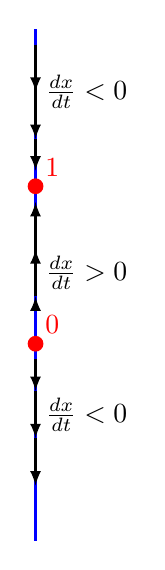
\begin{tikzpicture}[scale=2]
		% Vertical line
\draw[thick, blue] (0, -1.25) -- (0, 2);

% Equilibrium points
\fill[red] (0,0) circle (0.05) node[above right] {0};
\fill[red] (0,1) circle (0.05) node[above right] {1};

% Directional arrows
\draw[thick, ->, black, >=latex] (0, -0.1) -- (0, -0.3);
\draw[thick, ->, black, >=latex] (0, -0.3) -- node[right] {$\frac{dx}{dt}<0$} (0, -0.6);
\draw[thick, ->, black, >=latex] (0, -0.6) -- (0, -0.9);

\draw[thick, ->, black, >=latex] (0, 0.3) -- (0, 0.3);
\draw[thick, ->, black, >=latex] (0, 0.3) -- node[right] {$\frac{dx}{dt}>0$} (0, 0.6);
\draw[thick, ->, black, >=latex] (0, 0.3) -- (0, 0.9);

\draw[thick, ->, black, >=latex] (0, 1.3) -- (0, 1.1);
\draw[thick, ->, black, >=latex] (0, 1.9) -- node[right] {$\frac{dx}{dt}<0$} (0, 1.3);
\draw[thick, ->, black, >=latex] (0, 1.9) -- (0, 1.6);

	\end{tikzpicture}
\end{subfigure}
%\caption{The same cup of coffee. Two times.}
\end{figure}

	
	How to construct it?
	\begin{enumerate}
		\item (Nullclines) First, we need to draw the red lines, which represent the fixed points that solve $\dot{x} = 0$. 
		\item (Directional Arrows). To construct the directional arrows (that is, to determine how the points below and above $x(t)$ behave around $x^*$. This process involves differentiation. Just try a number and see the sign of $\dot{x}$.
	\end{enumerate}
	
	\subsection{System of 2 Linear Differential Equations} 
	Next, we move on to a system of 2 linear equations. Construction-wise, it is similar to the case of 1 variable, but we are now concerned with 2 variables instead of 1.
	
	Let us consider the system
	\begin{align}
		\begin{matrix}
			\dot{x} = a x + b y + \kappa_1, \\
		\dot{y} = c x + d y + \kappa_2. 
		\end{matrix} \label{phase_sys}
	\end{align}
	where $a < 0, b < 0, c < 0, d > 0, \kappa_1 > 0, \kappa_2 > 0$. You can see that
	\begin{align*}
		ad - bc < 0
	\end{align*}
	so the eigenvalues of the Jacobian of this system have OPPOSITE signs. The dynamical system is a ``saddle". Check Fig.~\ref{fig:exmaple_phase} while reading the following.
	\begin{enumerate}
		\item (A. Nullclines) We need to plot the nullclines, which are the loci $\dot{x}=0$ and $\dot{y}=0$. The first locus $\dot{x}=0$ is given by
		\begin{align*}
			y = - \frac{a}{b} x - \frac{\kappa_1}{b}
		\end{align*}
		since $a<0,b<0$, the locus is a straight line with a negative slope in the $(x,y)$ plane. The second locus $\dot{y} = 0$ is given by
		\begin{align*}
			y = - \frac{c}{d} x - \frac{\kappa_2}{d}
		\end{align*}
		since $c<0, d>0$, the locus is a straight line with a positive slope.
		\item (B. Steady State) The steady state is given by the intersection of the two nullclines. Let's call it $(x^*, y^*)$. Together with the nullclines, it divides the $(x,y)$ plane into 4 areas.
		\item (C. Directional Arrows) These arrows determine the direction of the system’s trajectories over time anywhere on the phase. Look at the system \eqref{phase_sys}.
		\begin{itemize}
			\item From the $\dot{x}$ function, we see that
			\begin{align*}
				\frac{d \dot{x}}{dx} = a < 0 && \frac{d \dot{x}}{dy} = b < 0  
			\end{align*}
			so $\dot{x}$ is decreasing in $x$ (and decreasing in $y$). Any point above the $\dot{x} = 0$ line must have $\dot{x} < 0$ and any point below $\dot{x}=0$ must have $\dot{x} > 0$. 
			\item From the $\dot{y}$ function, we see that
			\begin{align*}
				\frac{d \dot{y}}{dy} = d > 0 && \frac{d\dot{y}}{dx} = c < 0
			\end{align*}
			so $\dot{y}$ is increasing in $y$ (and decreasing in $x$). Any point above the $\dot{y} = 0$ line must have $\dot{x} > 0$ and any point below $\dot{x}=0$ must have $\dot{x} < 0$. 
			\item (D. Trajectories) Using the information above, we can draw trajectories that satisfy the system. These are solutions to the system.  To select a specific solution among all possible solutions, we will need to specify either an initial condition or a final condition. Among all the trajectories, we highlight the saddle path for the system. We know that such a saddle path exist because the eigenvalues of the system have opposite sign. The saddle path is the straight line that goes through the steady state.
		\end{itemize}
	\end{enumerate}
	
	\begin{figure}[ht]
		\centering
		\includegraphics[scale=0.4]{figs/phasediag.png}
		\caption{Phase diagram of the dynamical system \eqref{phase_sys} \citep{michaillat2023} .}
		\label{fig:exmaple_phase}
	\end{figure}
	
	\begin{ex}
		The exercises here are from \citet{michaillat2023, shone2002economic}
		\begin{enumerate}[label*=(\alph*)]
			\item (Problem 3) Consider the linear system of differential equations given by
			\begin{align*}
				\begin{pmatrix}
					\dot{x} \\ \dot{y}
				\end{pmatrix}
				=
				\begin{pmatrix}
					1 & 1 \\ 4 & 1
				\end{pmatrix}
				\begin{pmatrix}
					x \\ y
				\end{pmatrix}
			\end{align*}
			\begin{enumerate}[label=\arabic*.]
				\item Find the general solution of the system using either eigenvalue method, given $(x_0, y_0) = (\kappa_1, \kappa_2)$.
				\item Draw the phase diagram that plots the trajectories of the system
			\end{enumerate}
			\item The IS-LM continuous time model \citep[p.10.3]{shone2002economic}.
			\begin{align*}
				\text{(IS)}: & \ c(t) = a + b(1 - \tau) y(t) - h r(t), \\
				\text{(LM)}: & \ m(t) = k y(t) - u r(t)
			\end{align*}
			where $a > 0, b \in (0,1), \tau \in (0,1), h > 0$ and $c, a, b, \tau, y, h, r$ are consumption, fixed consumption, marginal propensity to consume, tax, real income, coeff. of investment, and interest rate. On the other hand, $k, u > 0$ control the demand for real money. Assume that the dynamics of the 2 markets are
			\begin{align*}
				\dot{y} = \alpha (c(t) - y(t)) \ \ (\alpha > 0), \\
				\dot{r} = \beta (m(t) - m_0) \ \ (\beta > 0)
			\end{align*}
			where income adjusts according to the excess demand in that market and interest rates adjust according to the excess demand in the money market.
			\begin{enumerate}[label=\arabic*.]
				\item Express the system explicitly in $\dot{y}, \dot{r}$.
				\item Find the fixed point $y^*, r^*$.
				\item Draw the phase diagram with the 2 loci $\dot{y} = 0$ and $\dot{r}=0$.
			\end{enumerate}
		\end{enumerate}
	\end{ex}	
	
	\subsection{System of 2 Nonlinear Differential Equations}
	In macroeconomics, most of the advanced dynamics fall into this category. These systems, in general, are difficult to solve explicitly. Nevertheless, without solving them, we can still characterize their properties by constructing the phase diagrams.  
	
	Consider the following nonlinear system that describes a typical growth model
	\begin{align}
		\begin{matrix}
			\dot{k} = f (k) - c - \delta k, \\
			\dot{c} = [ f'(k) - (\delta + \rho) ] c
		\end{matrix} \label{eq:sys_nonlin}
	\end{align}
	where $\rho > 0, \delta \in (0,1)$ are parameters, the capital stock $k(t)$ is a state variable with the initial value $k_0$ given and $c(t)$ is the control variable. The production function satisfies the Inada conditions as follows
	\begin{align*}
		&f(0) = 0, \\
		&f' > 0, f'' < 0, \\
		&\lim_{k\to\infty}  f'(k) = 0, \lim_{k\to 0} f'(k) = \infty.
	\end{align*}
	
	\begin{enumerate}
		\item (A. Nullclines) As always, we draw the nullclines. The $\dot{k}=0$ curve is defined by
		\begin{align*}
			c = f(k) - \delta k
		\end{align*}
		The $\dot{c} = 0$ curve is defined by 
		\begin{align*}
			f'(k) = \delta + \rho.
		\end{align*}
		In the $(k,c)$ plane, the $\dot{k}=0$ curve is concave in $k$ (because $f(k)$ is concave) while the $\dot{c}=0$ curve is just a vertical line.
		\item (B. Steady State) The intersection of these two loci is the steady state $(k^*, c^*)$.
		\item (C. Directional Arrows)  To do this, we investigate the partial derivatives
		\begin{align*}
			\frac{\partial \dot{k}}{\partial c} &= - 1 < 0, \\
			\frac{\partial \dot{c}}{\partial k} &= c \cdot f''(k) < 0
		\end{align*}
		What do they mean?
		\begin{itemize}
			\item The first equation says $\dot{k}$ is a decreasing function in $c$. So when $c$ increases, $\dot{k}$ turns more negative, implying that $k$ decreases (points above $\dot{k}=0$ moves leftward); and when $c$ decreases, the reverse happens, $k$ increases and the points move rightward.
			\item The second equation says $\dot{c}$ is decreasing in $k$. So when $k$ increases, $\dot{c}$ turns negative, implying that $c$ decreases (the points to the right of $\dot{c}=0$ moves downward); and when $k$ decreases, $c$ increases and the points to the left of $\dot{c}=0$ moves upward.
		\end{itemize}
		\item (D. Tracjectories)  The directional arrows drawn describe a saddle around the steady state. The
		only way for the economy to converge to the steady state is on the saddle path leading
		to it. This means that given any initial capital $k_0$, initial consumption $c_0$ is such that the
		pair $(k_0, c_0)$ lies on the saddle path.
	\end{enumerate}
	
	\begin{figure}[ht]
		\centering
		\includegraphics[scale=0.4]{figs/phasediag2.png}
		\caption{Phase Diagram of system \eqref{eq:sys_nonlin} \citep{michaillat2023}. }
		\label{fig:phase_diagram}
	\end{figure}
	\begin{figure}[H]
		\centering
		\begin{subfigure}[b]{0.45\linewidth}
			\includegraphics[width=\linewidth]{figs/romerramsey.png}
			\caption{ Trajectories \citep{romer2011advanced} }
		\end{subfigure}
		\begin{subfigure}[b]{0.45\linewidth}
			\includegraphics[width=\linewidth]{figs/phase_diagram.png}
			\caption{ A closer look. \\ Source code: \url{https://github.com/Mv77/Ramsey_growth/blob/master/Ramsey.py}  }
		\end{subfigure}
		\caption{ More on the trajectories of this model.}
	\end{figure}
	
	\subsubsection{Lineariziation around the Steady State}
	The phase diagram indicates that the system is a saddle around the steady state in Fig.~\ref{fig:phase_diagram}. We can also obtain this result by linearizing the nonlinear system \eqref{eq:sys_nonlin} using a first-order Taylor expansion about the steady state:
	\begin{align*}
		\dot{k} = \dot{k^*} + (k-k^*) \frac{\partial \dot{k}}{\partial k} + (c-c^*) \frac{\partial \dot{k}}{\partial c}, \\
		\dot{c} = \dot{c^*} + (k-k^*)\frac{\partial \dot{c}}{\partial k} + (c - c^*)\frac{\partial \dot{c}}{\partial c}.
	\end{align*}
	Since at the steady state $\dot{k^*} = \dot{c^*} = 0$, the system reduced to
	\begin{align*}
		\begin{pmatrix}
			\dot{k} \\ \dot{c}
		\end{pmatrix}
		=
		\J^*
		\begin{pmatrix}
			k - k^* \\ c - c^*
		\end{pmatrix}
	\end{align*}
	where $\J^*$ is the Jacobian matrix evaluated at the steady state
	\begin{equation*}
		{\J}^{*}= 
			\begin{pmatrix}
				\dfrac{\partial \dot{k}}{\partial k}\vert_{(k^{*},c^{*})}  & \dfrac{\partial \dot{k}}{\partial c}\vert_{(k^{*},c^{*})} \\ 
				\dfrac{\partial\dot{c}}{\partial k}\vert_{(k^{*},c^{*})} & \dfrac{\partial \dot{c}}{\partial c}\vert_{(k^{*},c^{*})}
		\end{pmatrix}.
	\end{equation*}
	More explicitly
	\begin{equation*}
		{\J}^{*}= 
		\begin{pmatrix}
			f'(k^*) - \delta & -1 \\
			c f''(k^*) & f'(k^*) - (\delta + \rho)
		\end{pmatrix}.
	\end{equation*}
	The result of evaluation is
	\begin{equation*}
		{\J}^{*}= 
		\begin{pmatrix}
			\rho & - 1 \\
			c f''(k) & 0
		\end{pmatrix}.
	\end{equation*}
	Calculating its determinant shows that
	\begin{align*}
		\det(\J^*) = c f''(k) < 0
	\end{align*}
	Thus, the 2 eigenvalues have opposite sign, so the system around the steady state is a saddle.
	
	\begin{ex}
		Given the system
		\begin{align*}
			\dot{k}(t) &= \frac{q(t) - 1}{\chi} k(t), \\
			\dot{q}(t) &= r q(t) - f'(k(t)) - 0.5 \chi^{-1} (q(t)-1)^2
		\end{align*}
		where $\chi, r > 0$ and 
		$$
			f(k(t)) = A k(t)^\alpha
		$$
		Draw the phase diagram and show that the steady state is a saddle point locally.
		\begin{figure}[ht]
			\centering
			\includegraphics[scale=0.35]{figs/phase_diagram2.png}
			\caption{Illustration with $r=0.1, \chi = 0.9, A = 2, \alpha = 0.3$.}
		\end{figure}
	\end{ex}
	
%	\begin{ex}[Holling-Tanner predatory-prey model (optional)]
%		From \citet[p.199]{shone2002economic}. Consider 
%		\begin{align*}
%			\text{(prey population):} &\ \dot{x} = x\left(1 - \frac{x}{6}\right) - \frac{6xy}{(8+8x)}, \\
%			\text{(predator population):} &\ \dot{y}= 0.2 y \left(1 - \frac{0.4 y}{x}\right)
%		\end{align*}
%		Find the fixed points. Check if any of the fixed points exhibit a stable limit cycle. \footnote{Hint: (i) $P1 = (6,0)$ and $P2 = (0.846, 2.114)$. (ii) Fixed point $P2$ exhibits a stable limit cycle.} A limit cycle is an isolated closed integral curve, which is also called an orbit. A limit cycle is asymptotically stable if all the nearby cycles tend to the closed orbit from both sides. Its stability conditions
%		\begin{enumerate}
%			\item eigenvalues have complex roots 
%		\end{enumerate}
%	\end{ex}	
	
	%===================== Dyn Opt ====================%
	
	\chapter{Dynamic Programming}
	There are 2 versions of dynamic optimization methods. The first deals with continuous time, where a variable is differentiable with time. The second deals with discrete time, where a variable is not differentiable with respect to time.
	
	\begin{figure}[h!]
\centering
\begin{subfigure}[b]{0.45\linewidth}
\includegraphics[width=\linewidth]{figs/concept1.png}
%\caption{Coffee.}
\end{subfigure}
\begin{subfigure}[b]{0.45\linewidth}
\includegraphics[width=\linewidth]{figs/concept2.png}
%\caption{More coffee.}
\end{subfigure}
\caption{Conceptualization of Time. Source: \href{https://www.youtube.com/watch?v=w9VM7is9cl8}{Klaus Prettner}}
\label{fig:concept}
\end{figure}

	In discrete time, we often use the Bellman method, while in continuous time, we often use the Hamiltonian method. Both of them are useful for analysis, and then we often use numerical simulations or a phase diagram to work out the dynamics of the model. The notes are based on \citet{chiang1992element, sydsaeter2008further, heer2009dynamic, campante2021advanced}, with references to a lot of online materials such as 
	\begin{enumerate}
		\item \url{http://www.chrisedmond.net/phd2019.html}
		\item \url{http://www.chrisedmond.net/hons2019.html}
		\item \url{https://pascalmichaillat.org/c3/}
	\end{enumerate}
	
	\section{Motivation (Ramsey) }
	This is a discrete-Time version of the optimal growth model \citep{ramsey1928mathematical}. 
	
	The household solves
	\begin{align*}
		\max_{c_t} & \sum^\infty_{t=0} \beta^t u(c_t), \\
		s.t. &\ c_t = f(k_t) - k_{t+1} + (1-\delta) k_t.
	\end{align*}
	Assume a nonzero initial condition, the constraint gives us the equation of motion of the state variable
	\begin{align*}
		&(\textbf{transition equation}) & k_{t+1} &= f(k_t) + (1-\delta)k_t - c_t, \\
		&(\textbf{initial condition}) & k_0 &> 0
	\end{align*}
	Find the solution for the optimal choice of $c_t$.
	
	\section{Lagrangian Method}
	The Lagrangian:

$$
    \mathcal{L} = \sum_{t=0}^{\infty} \beta^t u(c_t) + \sum_{t=0}^{\infty} \lambda_t \left[ f(k_t) + (1- \delta) k_t - k_{t+1} - c_t \right]
$$

Grouping all the summation and rewriting the Lagrangian:
$$
    \mathcal{L} = \sum_{t=0}^{\infty} \left[ \beta^t u(c_t) + \lambda_t \left( f(k_t) + (1- \delta)k_t - k_{t+1} - c_t \right) \right]
$$

The term inside the sum should be optimized at each point in time. The modified Lagrangian:
$$
    L = \beta^t u(c_t) + \lambda_t \left( f(k_t) + (1- \delta) k_t - k_{t+1} - c_t \right)
$$

FOC: (Note that $k_{t+1}$ appears twice at time $t$ and $t+1$)

\begin{align}
      &(c_t): \frac{\partial L}{\partial c_t} = \beta^t u'(c_t) - \lambda_t = 0  \label{eq:foc_c}  \ \                                                \\
      &(k_{t+1}): \frac{\partial L}{\partial k_{t+1}} = -\lambda_t + \lambda_{t+1} \left[ f'(k_{t+1}) + (1-\delta) \right] = 0 \label{eq:foc_k} \ 
\end{align}

By virtue of Eq.~\eqref{eq:foc_c}, we see that:

$$
    \beta^{t+1}u'(c_{t+1}) = \lambda_{t+1}
$$

Plugging back to Eq.~\eqref{eq:foc_k} and rearranging give us the Euler equation:

$$
    \frac{u'(c_t)}{u'(c_{t+1})} = \beta \left[ f'(k_{t+1}) + (1-\delta) \right]
$$

Consider the utility function $u(c_t) = \ln(c_t)$, we have:

$$
    \frac{c_{t+1}}{c_t} = \beta \left[f'(k_{t+1}) + (1-\delta)\right]
$$

In the steady-state, $c_{t+1} = c_t = \bar{c}$ and $k_{t+1} = k_t = \bar{k}$.  

Provided with a functional form of the production function $f(k)$, one can find the steady-state values of $\bar{c}, \bar{k}$ and then use backward induction to figure out the dynamics from a given $k_0$.
	
	\section{Bellman Method}
	The following steps describe Bellman's method.
	\begin{enumerate}
		\item Set up the Bellman equation
		\begin{align*}
			V(k_t) = \max \left[ u(c_t) + \beta V(k_{t+1}) \right]
		\end{align*}
		where one can replace
		\begin{align*}
			c_t = f(k_t) - k_{t+1} + (1-\delta) k_t
		\end{align*}
		so the problem changes from optimizing $c_t$ to optimizing $k_{t+1}$. Let's rewrite the Value Function as
		\begin{align*}
			V(k_t) = \max_{k_{t+1}} \left[ u(f(k_t) - k_{t+1} + (1-\delta)k_t) +\beta V(k_{t+1}) \right] 
		\end{align*}
		\item Maximizing the Value function wrt. the control variable $k_{t+1}$:
		\begin{align*}
			\frac{\partial V(k_t)}{\partial k_{t+1}} = 0 \Leftrightarrow \frac{\partial u(k_{t+1})}{\partial k_{t+1}} + \beta \blue{\frac{\partial V(k_{t+1})}{\partial k_{t+1}}} = 0 
		\end{align*}
		\item Do we know $\blue{\frac{\partial V(k_{t+1})}{\partial k_{t+1}}}$? Yes, it can be obtained by differentiating the Value Function to the state variable $k_t$
		\begin{align*}
			\frac{\partial V(k_t)}{\partial k_t} = (f'(k_t) + 1-\delta) u'( f(k_t) - k_{t+1} + (1-\delta)k_t ) 
		\end{align*}
		implying that
		\begin{align*}
			\frac{\partial V(k_{t+1})}{\partial k_{t+1}} &= (f'(k_{t+1}) + 1-\delta) u'\red{( f(k_{t+1}) - k_{t+2} + (1-\delta)k_{t+1} )} \\
			&= (f'(k_{t+1}) + 1-\delta)u'\red{ (c_{t+1})}
		\end{align*}
		\item Derive the Euler equation relating the dynamics of the choice variable.
		\begin{align*}
			\frac{u'(c_t)}{u'(c_{t+1})} = \beta (f'(k_{t+1}) + (1-\delta))
		\end{align*}
		where the transversality condition holds
		\begin{align*}
			\lim_{t\to 0} \beta^t u'(c_t) k_{t+1} = 0.
		\end{align*}
	\end{enumerate}
	
	\section{Ramsey-Cass-Koopsman Model}
	
	\chapter{Optimal Control}
	Also known as Continuous-Time Optimization. Let us consider the problem
	\begin{align}
		\max_{ \{c_t\}^T_{t=0} } e^{-(\rho-n) t} u(c_t)  dt, \\
		s.t. \ c_t + \dot{k}_t = f(k_t) - \delta k_t.
	\end{align}
	The control variable is $c_t$, and the state variable is $a_t$. Assume a nonzero initial condition, the constraint gives us the equation of motion for the state variable
	\begin{align*}
		&(\textbf{transition equation}) & \dot{k}_t &= f(k_t) - \delta k_t - c_t, \\
		&(\textbf{initial condition}) & k_0 &> 0
	\end{align*}

	
	\section{Lagrangian Method}
	Everything begins with the Lagrangian function. In fact, it's more intuitive to start here than going straight to Hamiltonian:

$$
    \mathcal{L} = \int_{0}^{\infty} e^{-\rho t} u(c(t)) dt + \int_{0}^{\infty} \lambda(t) \left[ f( k(t)) - \delta k(t) - c(t) - \dot{k}(t) \right] dt
$$

It's the sum of 2 integrals with the same boundary and the same variables (time), so we can sum them up and rewrite the Lagrangian:

$$
    \mathcal{L} = \int_{0}^{\infty} \left\{ e^{-\rho t} u(c(t)) + \lambda(t) \left[ f( k(t)) - \delta k(t) - c(t) - \dot{k}(t) \right] \right\} dt
$$

We want to maximize $c(t)$ with respect to $k(t)$, but $\dot{k}(t)$ is not independent with $k(t)$. So $\dot{k}(t)$ needs to be got rid of, and can somehow be expressed in terms of $k(t)$.

First, separate the $\dot{k}(t)$ term from the integral.

$$
    \mathcal{L} = \int_{0}^{\infty} \left\{ e^{-\rho t} u(c(t)) + \lambda(t) \left[ F( k(t)) - \delta k(t) - c(t)  \right] \right\} dt - \int_{0}^{\infty} \lambda(t)\dot{k}(t)dt
$$

Using integration by parts  for the second integral term:

$$
     \int_{0}^{\infty} \lambda(t) \dot{k}(t) dt                                               \\
     = \lambda(t) k(t) \Big|_0^\infty - \int_{0}^{\infty} \dot{\lambda}(t)k(t)dt              \\
     = \lambda(\infty) k(\infty) - \lambda(0) k(0) - \int_{0}^{\infty} \dot{\lambda}(t)k(t)dt 
$$

Notice that if $k$ at time $t=\infty$ is indeed $\infty$, and $\lambda(\infty)$ (the penalty term) is also non-zero, there is no reason to consume now. The household will wait until the very end of time close to infinity since the utility is essentially infinity. On the other hand, if $k$ at $t=\infty$ is $-\infty$, there is no reason to save, it's better to consume everything and leave nothing left. Such extreme cases would appear if $\lambda(\infty)k(\infty)$ is not bounded, and it will dominate everything.

To counter that problem, we introduce the transversality (no Ponzi scheme) condition.

$$
    \lim_{t\to\infty} \lambda(t)k(t) = 0
$$

We also assume $k(0)$ is given and is a constant (the economy needs something to start with), meaning it will disappear when we derive the FOC. As it is given, there should be no penalty term ($\lambda(0) = 0$). Thus, we have:

$$
    \int_{0}^{\infty} \lambda(t)\dot{k}(t) dt = - \int_{0}^{\infty} \dot{\lambda}(t) k(t) dt
$$

Plugging back to the Lagrangian $\mathcal{L}$, we obtain:

$$
    \mathcal{L} = \int_{0}^{\infty} \left\{ e^{-\rho t} u(c(t)) + \lambda(t) \left[ F( k(t)) - \delta k(t) - c(t)  \right] \right\} dt + \int_{0}^{\infty} \dot{\lambda}(t)k(t)dt 
$$

Sum them back to under 1 integral again:

$$
    \mathcal{L} = \int_{0}^{\infty} \left\{ e^{-\rho t} u(c(t)) + \lambda(t) \left[ F( k(t)) - \delta k(t) - c(t)  \right] +  \dot{\lambda}(t)k(t) \right\} dt 
$$

The Lagrangian enables us to maximize the function at each point in time, so we only care about maximizing the functional form inside the integral (we don't care about time anymore). Rewrite the term inside the integral as $L$, and call this the *modified Lagrangian*. The following two expressions are equivalent.

\begin{align}
     L = {e^{-\rho t} u(c(t)) + \lambda(t) \left[ f( k(t)) - \delta k(t) - c(t)  \right]} -  \lambda(t)\dot{k}(t)     \label{eq:foc_c2} \\                            
     L =  \underbrace{e^{-\rho t} u(c(t)) + \lambda(t) \left[ f( k(t)) - \delta k(t) - c(t)  \right]}_{\text{Hamiltonian}}+  \dot{\lambda}(t)k(t)  \label{eq:foc_k2}
\end{align}

Terminologically speaking: $c(t)$ is the control variable since it can jump (taking any value at any point in time). In contrast, $k(t)$ is the state variable because it accumulates over time. ${\lambda}(t)$ is the co-state variable (also known as *shadow price* in economics because it shows the marginal cost of violating the constraints at each point in time). 

Sticking with the Lagrangian method, we derive the FOC:

\begin{align}
     &(c(t)): \frac{dL}{d c(t)} = e^{-\rho t} u'(c(t)) - \lambda(t) = 0  \text{(using \eqref{eq:foc_c2})}     \\   
     &(k(t)): \frac{dL}{d k(t)} = \lambda(t) [ f'(k(t)) - \delta] + \dot{\lambda}(t) = 0 \ \text{(using Eq.\eqref{eq:foc_k2})} \\
     &(\lambda(t)): \frac{dL}{d \lambda(t)} = f(k(t)) - \delta k(t) - c(t) = 0 \ \text{(using \eqref{eq:foc_c2})}           
\end{align}

We need to get rid of $\lambda$. From $(c(t))$ condition, we derive:

$$
    \lambda(t) = e^{-\rho t} u'(c(t))
$$

Thus, $\dot{\lambda}(t)$ can be derived as:

$$
    \dot{\lambda}(t) = \frac{d \lambda(t)}{dt} = -\rho e^{-\rho t} u'(c(t)) + e^{-\rho t} u''(c(t)) \dot{c}(t)
$$

And we obtain:

$$
    \frac{\dot{\lambda}(t)}{\lambda(t)} = -\rho \frac{u'(c(t))}{u'(c(t))} + \frac{u''(c(t))}{u'(c(t))}\dot{c}(t) = - \rho + \frac{u''(c(t))}{u'(c(t))}\dot{c}(t)
$$

We can explicitly derive the condition for a functional form of $u$, especially with CRRA (constant relative risk aversion). For simplicity, let $u(c) = \ln(c)$, then $u'(c(t)) = \frac{1}{c(t)}$ and $u''(c(t)) = \frac{-1}{c^2(t)}$. Plugging back into the above equation, we obtain:

$$
    \frac{\dot{\lambda}(t)}{\lambda(t)} = -\rho - \frac{\dot{c}(t)}{c(t)} \ \ (5)
$$

From the FOC of $k(t)$, we know that:

$$
    - \frac{\dot{\lambda}(t)}{\lambda(t)} = f'(k(t)) - \delta
$$

Combining with Eq. (5) yields the Euler equation:

$$
\frac{\dot{c}(t)}{c(t)} = f'(k(t)) - \delta -\rho
$$

This condition constitutes the optimal path of consumption chosen by the household.

	\section{Hamiltonian}
	A cookbook method (Pontryagin’s maximum principle) for this problem.
		The maximum principle can be summarized as a series of steps with the economic intuition explained as follows \citep{campante2021advanced}.
	\begin{enumerate}
		\item Set at the present-value Hamiltonian
		\begin{align}
			H_t = u(c_t)e^{-\rho t} + \lambda_t ( \underbrace{f(k_t) - c_t - \delta k_t}_{\dot{k}_t})
		\end{align}
		where $\lambda_t$ is called the co-state variable. The Hamiltonian is similar to the way you obtain the Lagrangian (but without integral). The interpretation of the co-state variable $\lambda_t$ is the same as the Lagrangian multiplier. It tells you the marginal benefit of a marginal addition to the stock of the state variable $k_t$ (in economic jargon, it is called ``the shadow value/ price of the state variable"), which is also the value of the state variable at $t=0$.
				
		\item Take the FOC of Hamiltonian wrt the control variable(s)
		\begin{align}
			\frac{\partial H_t}{\partial c_t} = 0 \Leftrightarrow e^{-\rho t} u'(c_t) = \lambda_t. \label{eq:hc}
		\end{align}
		This is legitimate since the Hamiltonian is static at each $t$, so the optimal value of the choice variable should be done in a static optimization fashion. \eqref{eq:hc} states that the marginal utility gain from increasing consumption has to be equal to the marginal cost ($\lambda$) of not adding such amount to the stock of your assets (the state variable).
		
		\item Derive the optimal path of the state and co-state variable(s)
		\begin{align}
			\dot{k}_t &= \frac{\partial H_t}{\partial \lambda_t} = f(k_t) - c_t - \delta k_t, \label{eq:kdot} \\
			\dot{\lambda}_t &= \red{-} \frac{\partial H_t}{\partial k_t} = - \lambda_t (f'(k_t) - \delta) \label{eq:costate}
		\end{align}
		The Hamilton is static, but our model is dynamic. This means that, at any instant, we must figure out that whatever we leave for the next instant is consistent with optimization. This is the key insight into the problem. Furthermore, what we care about in an infinite time span can be broken down into a sequence of choices between the current instant and the next in an infinitesimally small time frame.
		
		To figure out that path, the maximization principle tells you that you need to satisfy the co-state equations. The first equation \eqref{eq:kdot} links one instant of the state variable to the next and must be satisfied at any time. The second equation \eqref{eq:costate} is an ``asset pricing" condition. Basically, the term $\dot{\lambda}_t$ is the appreciation in the marginal value of capital, so $-\dot{\lambda}_t$ is its depreciation. If you carry more capital to the next, its value should depreciate more as the volume increase. The term $\partial H/\partial k$, on the other hand, shows the marginal return of capital at this instant, contributing to the utility and production (which are encompassed in the Hamiltonian). Obviously, the equilibrium is brought by equalizing the two terms. (\href{https://www3.nd.edu/~nmark/Climate/CurrentValueHamiltonian.pdf}{Read more})
		
		\item Set the transversality condition
		\begin{align}
			\lim_{t\to\infty} \lambda_t k_t = 0. \label{eq:trans}
		\end{align}
		While the transition \eqref{eq:kdot}, and Euler equations (\eqref{eq:hc}, \eqref{eq:costate}) jointly govern the temporal behavior of consumption and capital (state variable), the initial and transversality conditions specify the state of the economy at the boundaries (i.e., $t = 0$ and $t = \infty$). Initially, the economy must start with something it can work with -- $k_0 > 0$. The transversality condition, in particular, prevents the over-accumulation of capital by requiring zero present value of the capital in an infinitely distant future. 
		
		In a finite time horizon (i.e., you must die at some point $T$), it makes sense that $\lambda(T) = 0$, so you have no incentive to save for the next period, you must consume everything. However, things get more complicated as we progress to the infinite horizon. Without this equation, households will keep accumulating capital indefinitely as capital has value $\lambda$ and households still have $k_t$ in expense, which implies that a steady state cannot be secured. To prevent this case from happening, condition \eqref{eq:trans} is necessary. The requirement is that at the limit $t\to\infty$, if the terminal capital has a positive present value, then you must consume it all to make $k(t) = 0$. Otherwise, it must have zero valuation $\lambda_t$ so that you are indifferent about leaving it unexploited. This transversality condition that imposes a non-negativity constraint on capital is also known as the ``no-Ponzi scheme" condition
		
		\item Derive the Euler equation relating the dynamics of the choice variable
		\begin{align}
			\rho - \frac{u''(c_t) \dot{c}_t}{u'(c_t)} = f'(k_t) - \delta. \label{eq:euler}
		\end{align}
		Ultimately, we are interested in the dynamic behavior of the control and state variable over time. This is done by taking \eqref{eq:hc} and differentiating both sides with respect to time (product and chain rule)
		\begin{align}
			\dot{\lambda}_t = -\rho e^{-\rho t} u'(c_t) + e^{-\rho t} u''(c_t) \dot{c}_t
		\end{align}
		which is the co-state variable. Substituting it to \eqref{eq:costate}, we have
		\begin{align*}
			-\rho e^{-\rho t} u'(c_t) + e^{-\rho t} u''(c_t) \dot{c}_t = -\lambda_t (f'(k_t)-\delta)
		\end{align*}
		and using \eqref{eq:hc} for $\lambda_t$, we obtain
		\begin{align*}
			-\rho e^{-\rho t} u'(c_t) + e^{-\rho t} u''(c_t) \dot{c}_t = - e^{-\rho t} u'(c_t) (f'(k_t)-\delta)
		\end{align*}
		Dividing both sides by $e^{-\rho t} u'(c_t)$, we obtain \eqref{eq:euler}. If we assume a log utility function, then it is easy to obtain the same result with Lagrangian
		\begin{align*}
			\frac{\dot{c}_t}{c_t} = f'(k_t) - \delta - \rho. 
		\end{align*}
	\end{enumerate}
	
	\section{Economic Applications}
	
	\section{Real Business Cycle (RBC)}
	
	
	\section{Programing}
	Sources:
	\begin{enumerate}
		\item \url{https://python-advanced.quantecon.org/discrete_dp.html}
		\item \url{https://macroeconomics.github.io/Dynamic%20Programming.html}
		\item \url{https://github.com/lnsongxf/NumEcon/tree/master/numecon/macro}
	\end{enumerate}
	\subsection{Backward Induction}
	\subsection{Value Function Iteration}
	\subsection{Policy Function Iteration}
	
		
%============ CHAPTER 1 ===========%
\chapter{Basics of Probability theory, Brownian motion and martingales}

\section{Probability theory}

\subsection{Probability space}
Let $\Omega$ be a (non-empty) sample space. A $\sigma$-algebra ($\sigma$-field) on $\Omega$ is a family of subsets of such that
\begin{itemize}
\item the empty set $\oslash$ belongs to $F$;
\item if $A$ belongs to $F$, then so does the complement $\Omega \backslash A$;
\item if $A_1$, $A_2$, ... is a sequence of sets in $F$, then their union $A_1 \cup A_2 \cup ...$ also belongs to $F$.
\end{itemize}

Let $F$ be a $\sigma$-algebra on $\Omega$. A Probability measure $P$, defined on $F$, is a function $P : F \rightarrow [0,1]$ such that
\begin{itemize}
\item $P(\Omega) = 1$;
\item if $A_1$, $A_2$, ... are pairwise disjoint sets (i.e. $A_i \cap A_j \cap ... = \oslash$ for $i \neq j$) belonging to $F$, then
$$P(A_1 \cup A_2 \cup ...)  = P(A_1) + P(A_2) + ...$$
\end{itemize}

The triple ($\Omega$, $F$, $P$) is called a \textbf{probability space}. The sets belonging to $F$ are called events.

\subsection{Random variables}
Let ($\Omega$, $F$, $P$) be a probability space. A \textbf{random variable} $X$ is a mapping from the sample space, $\Omega$, to another measurable space of possible values of $X$ (state space)
$$ X : \Omega \rightarrow R$$
with the property that $X^{-1}((-\infty, x]) = \{\omega \in \Omega : X(\omega) \leq x\} \in F$ for all $x \in R$. We say that $X$ is $F$-measurable.

\begin{figure}[H]
	\centering
	\includegraphics[scale=0.5]{Chapter 1/Chapter1_1.png}
	\caption{Mapping}
\end{figure}

The \textbf{distribution function} of $X$, $F_X : R \rightarrow [0,1]$ is defined by
$$ F_X(X) = P \{\omega \in \Omega : X(\omega) \leq x \} = P(X \leq x) = \mu_X((-\infty, x]) $$

\subsection{Expectations and conditional expectations}

$$E(g(X)) = \int_R g(x) f_X(x) dx  (= \int_R g(x) dF_X(x) = \int_R g(x) d\mu_X(x)) $$
$E(X | Y=y)$ is the mean of the conditional distribution of $X$ given $Y=y$.
$E(X | Y)$ is a random variable and the tower rule states:
$$E(E(X | Y)) = E(X)$$
Similarly,
$$E(E(X | Y_1,...,Y_n)) = E(X)$$
$E(X | Y_1,...,Y_n)$ is the optimal estimator of $X$ based on $Y_1,...,Y_n$ in the sense that for every function $h$
$$ E[ (X-E(X | Y_1,...,Y_n)^2 ] \leq E[ (X - h(Y_1,...,Y_n))^2 ] $$

\subsection{Stochastic processes}

A stochastic process, $X$, is a collection (family) of random variables
$$ X = \{X_t : t \in T \} = \{X_t(\omega), t \in T, \omega \in \Omega \} $$

Classification
\begin{itemize}
\item Discrete time stochastic processes, $T = \{0,1,2,...\}$;
\item Continuous time stochastic processes, $T = [0, \infty) (T = R^{+})$
\end{itemize}

$X$ is a function of two variables:
\begin{itemize}
\item for a fixed instant of time $t \in T$, it is a random variable $X_t = X_t(\omega), \omega \in \Omega$.
\item for a fixed random outcome $\omega \in \Omega$, it is a function of time $X_t = X_t(\omega), t \in T$ (trajectory, realisation or sample path).
\end{itemize}

\section{Brownian motion}

\subsection{Standard Brownian motion}
Let ($\Omega$, $F$, $P$) be a probability space. A standard Brownian motion (or Wiener process) under $P$ is a stochastic process, $\{W_t, t \geq 0 \}$, with continuous state space $R$ and $T = R^{+}$, and the following defining properties:
\begin{itemize}
\item $W_0 = 0$
\item independent increments, i.e. for every choice of $0 \leq t_0 < t_1 < ... < t_n, n \geq 1, W_{t_1} - W_{t_0}, W_{t_2} - W_{t_1}, ...,$ are independent random variables.
\item Gaussian increments, i.e. for $0 \leq s < t, W_t - W_s \sim N(0, t-s)$.
\item Continuous sample paths (no jumps)
\item stationary increments, i.e. for $0 \leq s < t$ and $h \geq 0$, $W_t - W_s \indist W_{t+h} - W_{s+h} $.
\end{itemize}

Statistical properties of standard Brownian motion:
\begin{itemize}
\item $E(W_t) = 0$
\item $Var(W_t) = t$
\item $Cov(W_s, W_t) = min(s,t)$
\item $Corr(W_s, W_t) = \sqrt{\frac{min(s,t)}{max(s,t}}$
\end{itemize}

\begin{figure}[H]
	\begin{subfigure}{0.5\textwidth}
		\centering
		\includegraphics[scale=0.5]{Chapter 1/Chapter1_2.png}
	\end{subfigure}
	\begin{subfigure}{0.5\textwidth}
		\centering
		\includegraphics[scale=0.5]{Chapter 1/Chapter1_3.png}
	\end{subfigure}
\end{figure}

Properties of standard Brownian motion:
\begin{itemize}
\item $W_t$ is a Markov process
\item $W_t$ is a martingale
\item $W_t$ returns infinitely often to 0 and to any other level
\item $W_t$ is 0.5 self-similar, i.e.
$$ (T^{\frac{1}{2}} W_{t_1}, ..., T^{\frac{1}{2}} W_{t_n}) \indist (W_{T\,\,t_1}, ..., W_{T\,\,t_n}) $$
for every $T>0$, any choice of $t_i \geq 0, i = 1, ..., n$ and $n \geq 1$.
\item $W_t^* = \frac{1}{\sqrt{c}} W_{ct}$ is also a standard Brownian motion (scaling property)
\item $W_t^{{**}} = t W_{1/t}$ is also a standard Brownian motion (inversion property)
\item $W_t$ has nowhere differentiable paths
\item $W_t$ has unbounded variation
\end{itemize}

\subsection{General Brownian motion}
General Brownian motion with drift parameter $\mu \in R$ and diffusion (volatility) parameter $\sigma > 0$ is a stochastic process, $\{X_t,t>0\}$,
$$ X_t = X_0 + \mu t + \sigma W_t $$
with Gaussian increments, $X_t - X_s \sim N(\mu(t-s), \sigma^2(t-s))$ for $0 \leq s < t$. We have
\begin{itemize}
\item $E(X_t - X_0) = \mu t$
\item $Var(X_t) = \sigma^2 t$
\item $Cov(X_s, X_t) = \sigma^2 min(s,t)$
\end{itemize}

\begin{figure}[H]
	\begin{subfigure}{0.5\textwidth}
		\centering
		\includegraphics[scale=0.5]{Chapter 1/Chapter1_4.png}
	\end{subfigure}
	\begin{subfigure}{0.5\textwidth}
		\centering
		\includegraphics[scale=0.5]{Chapter 1/Chapter1_5.png}
	\end{subfigure}
\end{figure}

\subsection{Geometric Brownian motion}
Geometric Brownian motion is a stochastic process, $\{S_t, t \geq 0\}$, such that
$$ S_t = e^{X_t} = S_0 e^{\mu t + \sigma W_t} $$
$ S_t \geq 0 $ for all $t \geq 0$ and $S_t \sim LogN(X_0+\mu t, \sigma^2 t)$.
\begin{itemize}
\item $E(S_t) = e^{X_0+(\mu+0.5\sigma^2)t}$
\item $Var(S_t) = e^{2X_0 + (2\mu + \sigma^2)t} (e^{\sigma^2 t} -1) = [E(S_t)]^2 (e^{\sigma^2 t}-1)$
\item $Cov(S_s,S_t) = e^{2X_0 + (\mu + 0.5\sigma^2)(s+t)}(e^{\sigma^2 t} -1)$, $0\leq s < t$.
\end{itemize}

\begin{figure}[H]
	\begin{subfigure}{0.5\textwidth}
		\centering
		\includegraphics[scale=0.5]{Chapter 1/Chapter1_6.png}
	\end{subfigure}
	\begin{subfigure}{0.5\textwidth}
		\centering
		\includegraphics[scale=0.5]{Chapter 1/Chapter1_7.png}
	\end{subfigure}
\end{figure}

\section{Martingales}

\subsection{Discrete time martingales}
A discrete time stochastic process, $\{X_n\}$, is said to be a martingale if
\begin{itemize}
\item $E(|X_n|) < \infty$ for all $n$
\item $E(X_n | X_0, ..., X_m) = X_m$ for all $m<n$
\end{itemize}

\begin{itemize}[label={$\Rightarrow$}]
\item The current value $X_m$ is the optimal estimator of its future value $X_n$. 
\item The expected change in the process is zero.
\item A martingale has a constant mean (driftless)
\end{itemize}
$$E(X_n) = E(E(X_n | X_0, ..., X_m)) = E(X_m) $$
\begin{example}
(risk-neutral probability): Suppose a share has price $S_t$ at time $t$, and assume for simplicity that it does not pay dividends. Let $S_t^* = e^{-rt} St$ be the price of the share discounted at the risk-free rate $r$. If, according to a partic-
ular probability distribution we assume for $S_t$, $S_t^* = e^{-rt} St$ is a martingale, then for $m<n$ find
$$ E\left( \frac{S_n}{S_m} | S_0, S_1, ..., S_m \right) = ? $$
\end{example}

\subsection{Filtration}
Let ($\Omega$, $F$, $P$) be a probability space on which a Brownian motion $W_t$, $t \geq 0$, is defined.

A \textbf{filtration} for the Brownian motion is a collection of $\sigma$-algebras, $\{F_t\}_{t\geq0}$, satisfying:
\begin{itemize}
\item for $0 \leq t < u$, $F_t \subset F_u \subset F$ (information accumulates). i.e. there is at least as much information available at the later time, $F_u$, as there is at the earlier time, $F_t$.
\item for each $t \geq 0$, $W_t$ is $F_t$-measurable (adaptivity), i.e. the information available at time $t$ is sufficient to evaluate $W_t$.
\item for $0\leq t<u$, $W_u - W_t$ is independent of $F_t$ (independence of future increments). i.e. any increment after time $t$ is independent of the information available at time $t$.
\end{itemize}
($\Omega$, $F$, $\{F_t\}_{t\geq0}$, $P$) is called the filtered probability space.

Let $F_t^X$ represent the information generated by the stochastic process $X=\{X_t, t\geq 0\}$ on the interval $[0, t ]$.

The filtration $\{F_t^X\}_{t \geq 0}$ such that $F_t^X = \sigma(X_s, s \leq t)$ is the smallest $\sigma$-algebra containing only the information obtained by observing the process itself on $[0,t]$, is the natural filtration associated with $\{X_t, t\geq 0\}$.

We say that the stochastic process $\{X_t, t \geq 0\}$ is adapted to the filtration  $\{F_t\}_{t \geq 0}$ if $\sigma(Xt) \subset F_t$ for all $t \geq 0$ (we also say that $X_t$ is $F_t$-measurable), i.e. if, based upon observations of the trajectory $\{X_s, 0 \leq s \leq t\}$ , it is possible to decide whether a given event $A \in F_t$ has occurred or not (or equivalently, whether the information in $F_t$ is sufficient to determine the trajectory $\{X_s, 0 \leq s \leq t\}$ ).

If $\{X_t\}_{t \geq 0}$ is adapted to the filtration $\{F_t\}_{t \geq 0}$, then $\{f(X_t)\}_{t \geq 0}$ is also adapted to $\{F_t\}_{t \geq 0}$.

\begin{example}
Consider the possible outcome of three days share price, i.e.
\begin{figure}[H]
	\centering
	\includegraphics[scale=0.6]{Chapter 1/Chapter1_8.png}
\end{figure}
\begin{enumerate}[label=(\alph*)]
\item Write down $\Omega$, $F_0$, $F_1$, $F_2$ and $F_3$.
\item Suppose $u=\frac{1}{d}$, so that $ud = du = 1$. Write down $\sigma(S_2)$.
\end{enumerate}
\end{example}

Properties of conditional expectation (with filtration):
\begin{itemize}
\item $E(c_1X_1 + c_2X_2 | F) = c_1 E(X_1 | F) + c_2 E(X_2 | F)$
\item $E( E(X|F) ) = E(X)$
\item $E(X|F) = E(X)$ if $X$ is independent of $F$
\item $E(X|F) = X$ if $X$ is $F$-measurable, i.e. $\sigma(X) \subset F$
\item $E(XZ|F) = XE(Z|F)$ if $X$ is $F$-measurable
\item $E(X|F) = E(E(X|F)|F') = E(E(X|F')|F)$ if $F \subset F'$
\end{itemize}

\subsection{Continuous time martingales}
A continuous time stochastic process, $\{X_t\}$, is said to be a martingale with respect to a filtration $\{F_t\}_{t\geq 0}$ if
\begin{itemize}
\item $X_t$ is adapted to the filtration $\{F_t\}_{t\geq 0}$
\item $E(|X_t|) < \infty$ for all $t$
\item $E(X_t | F_s) = X_s$ for all $s \leq t$
\end{itemize}

\begin{itemize}[label={$\Rightarrow$}]
\item The current value $X_s$ is the optimal estimator of its future value $X_t$. 
\item The expected change in the process is zero.
\item A martingale has a constant mean (driftless)
\end{itemize}
$$E(X_t) = E(E(X_t | F_s)) = E(X_s) \text{ for all } s \leq t$$
\begin{example}
Let $X_t = e^{\lambda W_t - 0.5 \lambda^2 t}$, where $\lambda$ is a constant. Show that $X_t$ is a martingale wrt $\{F_t\}_{t\geq 0}$, the filtration associated with $W_t$.
\end{example}

\section{Exercises}
\begin{ex}
Show that $X_t = W_t^2 - t$ is a martingale wrt $\{F_t\}_{t\geq 0}$, the filtration associated with $W_t$.
\end{ex}

%============ CHAPTER 2 ===========%
\chapter{Stochastic calculus and Ito process}

\textbf{Stochastic calculus} is a branch of mathematics that operates on stochastic processes.

It allows a consistent theory of integration to be defined for integrals of stochastic processes with respect to stochastic processes and helps to describe continuous-time stochastic processes using stochastic differential equations (SDE).

\section{Ito integral}

Suppose that $W_t$ is a Brownian motion and that $C_t$ is a stochastic process adapted to the natural filtration of the Brownian motion.

A stochastic integral of the type
$$I(C) = \int_a^b C_s dW_s $$
is called an Ito integral.

A direct approach to $I(C)$ is doomed to failure. Because $W_t$ has nowhere differentiable paths and has unbounded (first-order) variation.


However, such Ito integrals can be given a meaning for a suitable class of $C_s$ through successive aproximations by step functions.

\subsection{Example}

Consider the integral
\begin{equation}
\int_0^t W_s dW_s
\end{equation}
and the Riemann-Stieltjes sums
$$ S_n = \sum_{i=1}^n W_{t_{i-1}} (W_{t_i} - W_{t_{i-1}}) $$
where $\tau_n:0 = t_0 < t_1 < ... < t_{n-1} = t$ is a partition of $[0,t]$ with $||\tau_n || = max_{j=1,...,n}(t_j - t_{j-1})$.

Note that
$$ S_n = \frac{1}{2}W_t^2 - \frac{1}{2}\sum_{i=1}^n (W_{t_i} - W_{t_{i-1}})^2 = \frac{1}{2}W_t^2 - \frac{1}{2}Q_n(t) $$
where $Q_n(t) = \sum_{i=1}^n (W_{t_i} - W_{t_{i-1}})^2$ is the sampled quadratic variation of Brownian motion.

\vspace{4pt}
Proof:
\begin{align*}
S_n &= W_0(W_1- W_0) + W_1 (W_2 - W_1) + ... + W_{n-1} (W_n - W_{n-1}) \\
Q_n &= (W_1 - W_0)^2 + (W_2-W_1)^2 + ... + (W_n - W_{n-1})^2 \\
&= W_0^2 + 2W_1^2 + 2W_2^2 + ... + 2W_{n-1}^2 + W_n^2 - 2W_0W_1 - 2W_1W_2 - ... - 2W_{n-1}W_n \\
&= -2(W_0W_1 + W_1W_2 + ... + W_{n-1}W_n - W_0^2 - W_1^2 - ... - W_{n-1}^2) + W_n^2 - W_0^2 \\
&= -2S_n - W_0^2 + W_n^2 \\
&= -2S_n + W_n^2 \\
\therefore S_n &= \frac{1}{2}W_n^2 - \frac{1}{2}Q_n
\end{align*}

$$E[Q_n(t)] = \sum_{i=1}^n E[(W_{t_i} - W_{t_{i-1}})^2] = t$$
$$Var[Q_n(t)] = \sum_{i=1}^t Var[(W_{t_i} - W_{t_{i-1}})^2] = 2 \sum_{i=1}^n (t_i - t_{i-1})^2 \,\,\,\,\,(\leq 2 ||\tau_n|| \sum_{i=1}^n (t_i - t_{i-1}) = 2||\tau_n||t ) $$

Recall
\begin{itemize}
\item Convergence in probability
$$ \lim_{n \rightarrow \infty} P(|X_n - X| \geq \epsilon) = \lim_{n \rightarrow \infty} P(\{\omega:|X_n(\omega) - X(\omega)| \geq \epsilon\}) = 0 \text{  for any } \epsilon > 0 $$
\item Convergence in $r$-th mean
$$ \lim_{n \rightarrow \infty} E(|X_n - X|^r) = 0 $$
\end{itemize}
Mean square convergence ($r = 2$) implies convergence in probability.

We have
$$ E[(Q_n(t) - t)^2] = E[(Q_n(t)- E[Q_n(t)])^2] = Var[Q_n] \rightarrow 0 \text{  as  } ||\tau_n|| = max_{i=1,...,n}(t_i - t_{i-1}) \rightarrow 0 $$
i.e. we have shown that $Q_n(t)$ converges to $t$ in mean square sense, hence in probability.
$$ S_n = \frac{1}{2}(W_t^2 - Q_n(t)) \rightarrow \frac{1}{2}(W_t^2 - t) $$
Hence
\begin{align*}
(W_{t+dt}-W_t)^2 &= (dW_t)^2 = dt \\
dW_t dt &= 0 \\
(dt)^2 &= 0
\end{align*}
Hence, we could define integral (2.1) as a mean square limit
$$ \int_0^t W_s dW_s = \frac{1}{2}(W_t^2 - t) $$

We have shown that
$$ \lim_{n \rightarrow \infty, ||\tau_n|| \rightarrow 0} \sum_{i=1}^n (W_{t_i} - W_{t_{i-1}})^2 = t $$

So, in terms of differentials we write informally
\begin{equation}
(W_{t+dt} - W_t)^2 = (dW_t)^2 = dt
\end{equation}
Furthermore, we have
\begin{align}
dW_t dt = 0 \nonumber \\
(dt)^2 = 0
\end{align}

\subsection{Simple processes}
The stochastic process $\{C_t, t\in [0, T]\}$ is said to be \textbf{simple} if it satisfies the following properties
\begin{itemize}
\item There exist a partition $\tau_n$ :and a sequence, $Z_i$, $i = 1,...,n$ of random variables such that
$$ C_t = \begin{cases}
Z_i, \text{     if } t_{i-1} \leq t < t_i \\
Z_n, \text{     if } t = T
\end{cases} $$
\item The sequence $Z_i$ is adapted to the natural filtration $F_{t_{i-1}} = \sigma (W_s, s \leq t_{i-1} ), \,\, i = 1, ... , n$.
\item $E[Z_i^2] < \infty$ for all $i$
\end{itemize}

The Ito integral of a simple process $C$ on $[0, T]$ is given by
\begin{equation}
\int_0^T C_s dW_s = \sum_{i=1}^n C_{t_{i-1}} (W_{t_i} - W_{t_{i-1}}) = \sum_{i=1}^n Z_i (W_{t_i} - W_{t_{i-1}})
\end{equation}

The Ito integral of a simple process $C$ on $[0,t]$, $t_{k-1} \leq t \leq t_k$, is given by
\begin{equation}
\int_0^t C_s dW_s = \int_0^T C_s 1_{[0,t]}(s) dW_s = \sum_{i=1}^{k-1} Z_i (W_{t_i} - W_{t_{i-1}}) + Z_k (W_t - W_{t_{k-1}})
\end{equation}

\begin{example}
Let $C_t = 1$ for $t \in [0,T]$. Then we have
\begin{equation}
\int_0^t C_s dW_s = \int_0^t dW_s = W_t - W_0 = W_t
\end{equation}
\end{example}

Let $\sigma(t)$ be a given deterministic function of time, then it can be shown that
$$ \int_0^t \sigma(s) dW_s \sim N \left(0, \int_0^t \sigma^2(s) ds \right) $$

\begin{example}
Let $C_t = \begin{cases}
1, \text{   if } 0 \leq t < t_1 \\
2, \text{   if } t_1 \leq < T \\
0, \text{   otherwise}
\end{cases}$

Then
$$ \int_0^t C_s dW_s = \begin{cases}
\int_0^t dW_s = W_t \text{,   if } 0 \leq t < t_1 \\
\int_0^{t_1} dW_s + \int_0^{t_1} dW_s + \int_{t_1}^t 2dW_s = 2W_t - W_{t_1} \text{,   if } t_1 \leq t < T
\end{cases} $$
\end{example}

\begin{example}
Let $C_t = \begin{cases}
W_{t_{i-1}}, \text{   if } 0t_{i-1}\leq t < t_i \\
W_{t_{n-1}}, \text{   if } t = T
\end{cases}$

Then, for $t_{k-1} \leq t < t_k$, we have
$$ \int_0^t C_s dW_s = \sum_{i=1}^{k-1} W_{t_{i-1}} (W_{t_i} - W_{t_{i-1}}) + W_{t_{k-1}} (W_t - W_{t_{k-1}}) $$
\end{example}

\subsection{General Ito integral}
Let the stochastic process $\{C_t, t\in [0, T]\}$ be such that
\begin{itemize}
\item $C_t$ is adapted to the natural filtration $F_t = \sigma (W_s, s \leq t)$, $t \in [0,T]$.
\item $\int_0^T E[C_s^2] ds < \infty$.
\end{itemize}

Then $C_t$ can be approximated by a sequence $C^{(n)}$ of simple processes such that
$$ \int_0^T E[C_s - C_s^{(n)}]^2 ds \xrightarrow{n \rightarrow \infty} 0 $$

It can be shown that the mean square limit, $I_t(C)$ , such that
$$ E \sup_{0 \leq t \leq T} [I_t(C) - I_t(C^{(n)})]^2 = E \sup_{0 \leq t \leq T} [\int_0^t C_s dW_s - \int_0^t C^{(n)} dW_s]^2 \xrightarrow{n \rightarrow \infty} 0 $$
exists and is called the \textbf{Ito stochastic integral} of C.

\begin{figure}[H]
	\centering
	\includegraphics[scale=0.4]{Chapter 2/Chapter2_1.png}
	\caption{Illustration of Ito integral}
\end{figure}

An Ito stochastic integral has some properties:
\begin{itemize}
\item The Ito stochastic integral is linear.

For constants $c_1$, $c_2$ and processes $C^{(1)}$ and $C^{(2)}$ on $[0, T]$
$$ \int_0^t (c_1 C_s^{(1)} + c_2 C_s^{(2)}) dW_s = c_1 \int_0^t C_s^{(1)} dW_s + c_2 \int_0^t C_s^{(2)} dW_s $$
\item The Ito stochastic integral is linear on adjacent intervals.

For $0 \leq t \leq T$
$$ \int_0^T C_s dW_s = \int_0^t C_s dW_s + \int_t^T C_s dW_s $$
\end{itemize}

Denote $I_t(C) = \int_0^t C_s W_s$, $t \in [0, T]$. The stochastic process $I_t(C)$
\begin{itemize}
\item is a martingale with respect to the natural Brownian filtration $\{F_t, t \in [0, T]\}$, i.e. for $s<t$
$$ E[I_t(C) | F_s] = I_s(C) $$
\item has expectation zero
$$ E[I_t(C)] = E[I_0(C)] = 0 $$
\item satisfies the isometry property
$$ E[(\int_0^t C_s dW_s)^2] = \int_0^t E[C_s^2] ds $$
\item has continuous sample paths
\end{itemize}

\section{Ito formula}

\subsection{Diffusion process}
Stochastic differential equations (SDE) can be used to define a continuous time stochastic processes.

\textbf{Diffusion processes}, $X_t$, are processes that satisfy the Ito SDE
\begin{equation}
X_t = X_0 + \int_0^t \mu(s,X_s) ds + \int_0^t \sigma(s,X_s) dW_s
\end{equation}
or expressed in differential form
\begin{equation}
dX_t = \mu(t,X_t) dt + \sigma(t,X_t) dW_t
\end{equation}

For example, a Brownian motion takes the form
$$ dX_t = \mu dt + \sigma dW_t $$

\subsection{Ito formula}
Let $f(t, x)$ be a deterministic, twice partially differentiable function with continuous partial derivatives. Let $X_t$ be a diffusion process adapted to $W_t$. Define the process $Z_t = f(t, X_t)$. The stochastic differential (the SDE) of $Z_t$ is given by
\begin{equation}
df(t,X_t) = \left[ \frac{\partial f}{\partial t} + \mu(t,X_t) \frac{\partial f}{\partial x} + \frac{1}{2} \sigma^2(t,X_t) \frac{\partial^2 f}{\partial x^2} \right] dt + \sigma(t,X_t) \frac{\partial f}{\partial x} dW_t
\end{equation}

$Z_t$ is again a diffusion process.

\vspace{15pt}
Proof: Make a second-order Taylor expansion
\begin{equation}
df(t,X_t) = \frac{\partial f}{\partial t}dt + \frac{\partial f}{\partial x}dX_t + \frac{1}{2} \frac{\partial^2 f}{\partial t^2} (dt)^2 + \frac{1}{2} \frac{\partial^2 f}{\partial x^2} (dX_t)^2 + \frac{\partial^2 f}{\partial t \partial x}dt\,\,dX_t 
\end{equation}
As $dX_t = \mu(t,X_t) dt + \sigma(t,X_t) dW_t$,
$$ (dX_t)^2 = (\mu(t,X_t) dt)^2 + (\sigma(t,X_t) dW_t)^2 + 2\mu(t,X_t)\sigma(t,X_t)dt dW_t $$
For small $dt$, we have $(dt)^2 \rightarrow 0$, $dt dW_t \rightarrow 0$ and $(dW_t)^2 \rightarrow dt$.
$$ \therefore (dX_t)^2 = \sigma^2(t,X_t)dt $$
Plugging everything in completes the proof.

\pagebreak

\begin{example}
Let $f(x) = x^2$. Find the SDE for $W_t^2$.

\vspace{15pt}
\textbf{Solution:}
Let $X_t = W_t$. Therefore $dX_t = dW_t$ and it is a diffusion process with $\mu = 0$ and $\sigma = 1$.
Then 
$$ \frac{\partial f}{\partial x} = 2x \,\,\,\,\,\,\,\,\,\, \frac{\partial^2 f}{\partial x^2} = 2 \,\,\,\,\,\,\,\,\,\,
\frac{\partial f}{\partial t} = 0 $$
\begin{align*}
dW_t^2 = df &= \left( \frac{\partial f}{\partial t} + \mu \frac{\partial f}{\partial x} + \frac{1}{2} \sigma^2 \frac{\partial^2 f}{\partial x^2} \right) dt + \sigma \frac{\partial f}{\partial x} dW_t \\
&= ( 0 + 0 + \frac{1}{2}\times 1^2 \times 2)dt + 1 \times 2 W_t dW_t \\
&= dt + 2W_t dW_t
\end{align*}
\begin{align*}
\int_0^t dW_s^2 &= \int_0^t ds + \int_0^t 2W_s dW_s \\
W_t^2 - W_0^2 &= t + 2\int_0^t W_s dW_s \\
\therefore \int_0^t W_s dW_s &= \frac{1}{2}(W_t^2 - t)
\end{align*}
\end{example}

\begin{ex}
Let $f(t,x) = x^2-t$ and $X_t = W_t$. Find the SDE for $W_t^2-t$ and compare the resulting SDE with Example 2.5.
\end{ex}

\begin{ex}
Consider a particular form of geometric Brownian motion $S_t = f(t,W_t) = e^{(\alpha - 0.5 \sigma^2)t + \sigma W_t}$, where $\alpha$ and $\sigma > 0$ are constants. Find the SDE for $S_t$.
\end{ex}

\subsection{Geometric Brownian motion revisited}
A standard model for the price of a risky asset like a stock is
$$ \frac{dS_t}{S_t} = \alpha dt + \sigma dW_t $$
where $\alpha, \sigma >0$. Consider the SDE
\begin{equation}
dS_t = \alpha S_t dt + \sigma S_t dW_t
\end{equation}
Suppose $S_t = f(t,W_t)$. Comparing (2.11) with (2.9) yields the following system of two partial differential equations
$$ \frac{\partial f}{\partial t}(t,x) + \frac{1}{2}\frac{\partial^2 f}{\partial x^2}(t,x) = \alpha f(t,x) $$
$$ \frac{\partial f}{\partial x}(t,x) = \sigma f(t,x) $$
The second equation gives
$$ \frac{\partial f}{\partial x}(t,x) = \sigma f(t,x) \Longrightarrow \frac{\partial f(t,x)}{f(t,x)} = \sigma \partial x \Longrightarrow f(t,x) = f(t,0)e^{\sigma x} $$
Substituting into the first gives
$$ \frac{\partial f}{\partial t}(t,0)e^{\sigma x} + \frac{1}{2}f(t,0)\sigma^2 e^{\sigma x} = \alpha f(t,0) e^{\sigma x} \Longrightarrow \frac{\partial f}{\partial t}(t,0) + \frac{1}{2}f(t,0)\sigma^2 = \alpha f(t,0) \Longrightarrow$$
$$ \frac{\partial f}{\partial t}(t,0) = \left(\alpha - \frac{1}{2}\sigma^2 \right) f(t,0) \Longrightarrow \frac{\partial f(t,0)}{f(t,0)} = \left(\alpha - \frac{1}{2}\sigma^2 \right) \partial t \Longrightarrow f(t,0) = f(0,0) e^{(\alpha - \frac{1}{2}\sigma^2)t} $$
Thus we obtain
$$f(t,x) = f(t,0)e^{\sigma x} = f(0,0)e^{(\alpha - \frac{1}{2}\sigma^2)t+\sigma x} $$
Since $S_0 = f(0,W_0) = f(0,0)$, we have
$$ S_t = f(t,W_t) = S_0 e^{(\alpha - \frac{1}{2}\sigma^2)t + \sigma W_t} $$
Hence, the solution of (2.11) is a geometric Brownian motion with drift parameter $\mu = \alpha - \frac{1}{2}\sigma^2$ and diffusion parameter $\sigma$. Thus $\frac{S_t}{S_0} \sim LogN( (\alpha-\frac{1}{2}\sigma^2)t, \sigma^2 t)$ and
$$ E\left[ \frac{S_t}{S_0} \right] = e^{\alpha t} \text{           } Var\left[ \frac{S_t}{S_0} \right] = e^{2\alpha t}(e^{\sigma^2t}-1) $$

\subsection{Mean-reverting process}
A standard model for the spot rate of interest (Vasicek model) is
$$ dr_t = -\alpha (r_t -\mu)dt + \sigma dW_t $$
where $\alpha, \sigma>0$, $\mu \in R$.

Let $X_t = r_t-\mu$. Consider the SDE
\begin{equation}
dX_t = -\alpha X_t dt + \sigma dW_t
\end{equation}
Suppose $Y_t = e^{\alpha t}X_t = f(t,X_t)$ where $f(t,X_t) = e^{\alpha t}x$ and $X_t$ is a diffusion process with $\mu(t,X_t) = -\alpha X_t$ and $\sigma(t,X_t) = \sigma$. Apply Ito's lemma to $Y_t$ yields
$$ dY_t = [\alpha e^{\alpha t}X_t-\alpha e^{\alpha t}X_t+0]dt + [e^{\alpha t}]\sigma dW_t $$
which is equivalent to
$$ d(e^{\alpha t} X_t) = \sigma e^{\alpha t} dW_t $$
Integrating between 0 and $t$ we obtain
$$\int_0^t d(e^{\alpha s}X_s) = \sigma \int_0^t e^{\alpha s} dW_s \Longrightarrow e^{\alpha t}X_t - e^{\alpha 0}X_0 = \sigma \int_0^t e^{\alpha s} dW_s $$
Finally we have
$$ X_t = X_0e^{\alpha t} + \sigma e^{-\alpha t} \int_0^t e^{\alpha s} dW_s $$
or
$$ r_t = r_0e^{-\alpha t} + \mu(1-e^{-\alpha t}) + \sigma e^{-\alpha t} \int_0^t e^{\alpha s} dW_s $$
Properties:
\begin{itemize}
\item $E[X_t] = X_0 e^{-\alpha t}$
\item $Var[X_t] = \frac{\sigma^2}{2\alpha}(1-e^{-2\alpha t})$
\end{itemize}
The mean-reverting (Ornstein-Uhlenbeck) process is a Gaussian process with
$$X_t \sim N(X_0e^{-\alpha t}, \frac{\sigma^2}{2\alpha}(1-e^{-2\alpha t}))$$
The asymptotic (long term $t \rightarrow \infty$) distribution is $N(0,\frac{\sigma^2}{2\alpha})$.


%============ CHAPTER 3 ===========%
\chapter{Introduction to derivative securities}

\section{Derivative securities}

\subsection{Definitions}
A \textbf{derivative security} is a security (financial contract) whose value is derived from that of another underlying, more basic, security.

Underlying securities can include stock, bond, index, interest rate, currency, commodity and so on.

Common securities:
\begin{itemize}
\item Forwards
\item Futures
\item Options
\item Swaps
\end{itemize}

A \textbf{forward contract} is an agreement between two parties to buy (or sell) an asset at a pre-specified future date for a delivery (forward) price agreed in advance.

A \textbf{futures contract} is a standardised forward contract traded on an exchange.

An \textbf{option} is a financial contract which conveys the right, but not the obligation, to engage in a specific transaction, on some underlying security, at or by a pre-specified future date at a specified price.
\begin{itemize}
\item Call: right to buy the underlying asset
\item Put: right to sell the underlying asset
\item European: the right can be exercised only at maturity
\item American: the right can be exercised at any time prior to or at maturity
\end{itemize}

\subsection{Assumptions}
Before diving into derivative pricing models, we need to make several assumptions:
\begin{itemize}
\item No market frictions: no transaction costs, no bid/ask spread, no taxes, no restrictions on short sales 
\item The same risk-free interest for borrowing and lending
\item Competitive markets: market participants act as price takers
\item Rational agents: market participants prefer more to less
\item No arbitrage
\end{itemize}

An \textbf{arbitrage} opportunity is a situation where we can make sure profit with no risk. Namely,
\begin{itemize}
\item Start at time 0 with a zero-cost portfolio
\item At some future time $T$
\begin{itemize}[label=$\circ$]
\item the probability of a loss is 0
\item the probability that we make a strictly positive profit is strictly greater than 0
\end{itemize}
\end{itemize}
The principle of no arbitrage states that arbitrage opportunities do not exist. Any two assets (or combination of assets) that have exactly the same cash flows (give exactly the same payments) must have the same price ("Law of one price").

\section{Forward contracts}

\begin{itemize}
\item $S_t$ is the price of the underlying (share) at time $t$
\item $T$ is the expiry date (maturity)
\item $F_{0,T}$ is the forward price (the price the buyer agrees to pay at time $T$) at time $t=0$
\item $r$ is the risk-free continuously-compounding rate of interest (constant)
\end{itemize}

\subsubsection*{Non-dividend-paying share}

The forward price $F_{0,T}$ should be set so that the value of the contract at time $t = 0$ is zero.
\begin{equation}
F_{0,T} = S_0 e^{rT}
\end{equation}

\begin{example}
A share of XYZ company has a current price of \$42.60. A three-month forward contract on it is issued. Calculate the forward price given that the yield available on three-month government securities is 6\% per annum effective.

\vspace{15pt}
\textbf{Solution:}
Here $S_0 = \$42.60$, $T = \frac{3}{12}$ and $r = 0.06$.
Apply the formula and we get
$$ F_{0,\frac{3}{12}} = \$ 42.60 \times e^{0.06 \times \frac{3}{12}} = \$ 43.24 $$
\end{example}

\subsubsection*{Discrete dividend-paying share}

Suppose a stock is expected to make multiple dividend payments, $D_{t_i}$, at times $t_i$, $i=1,...,n$ throughout the life of the forward contract.
\begin{equation}
F_{0,T} = S_0 e^{rT} - \sum_{i=1}^n e^{r(T-t_i)}D_{t_i} = \left(S_0 - \sum_{i=1}^n e^{-rt_i} D_{t_i} \right) e^{rT} = (S_0 - I) e^{rT}
\end{equation}

\begin{example}
Suppose XYZ stock costs \$100 today and is expected to pay a \$1.25 quarterly dividend, with the first coming 3 months from today and the last just prior to the delivery of the stock. Suppose the annual continuously compounded risk-free rate is 10\%. Calculate the delivery (forward) price of a 1-year forward contract on the stock.

\vspace{15pt}
\textbf{Solution:}
Here $S_0 = \$100$, $r=0.1$, $T = 1$ and Dividend $=1.25$.
Therefore
\begin{align*}
F_{0,1} &= \$100 e^{0.1 \times 1} - \$1.25 (e^{0.1\times \frac{9}{12}} + e^{0.1\times \frac{6}{12}} + e^{0.1\times \frac{3}{12}} + e^{0.1\times \frac{0}{12}}) \\
&= \$ 105.32
\end{align*}
\end{example}

In the example, if short-selling is allowed, we can have the following two portfolios:
\begin{table}[H]
\centering
\begin{tabular}{c|c}
Portfolio A & Portfolio B \\
Take out forward at price $F_{0,T}$ & Borrow \$100 and buy share \\
 & \\
After 1 year & After 1 year \\
$-F_{0,T}$ cash $+ 1$ share & $-100e^{0.1}$ cash $+1$ share \\
& + dividends of $1.25(1+e^{0.025}+e^{0.05}+e^{0.075})$
\end{tabular}
\end{table}


\vspace{15pt}
\subsubsection*{Continuous dividend-paying share}

Suppose a dividend is being paid continuously at a rate proportional to the level of the index, i.e. suppose $q$ is a constant annualised dividend yield.
\begin{equation}
F_{0,T} = S_0 e^{(r-q)T}
\end{equation}

\subsubsection*{Currency exchange}

Suppose one has 1\texteuro at time 0. Let the euro-denominated interest rate is $r_e$ and the exchange rate today is $S_0 \$ /$\texteuro.
\begin{equation}
F_{0,T} = S_0 e^{(r-r_e)T}
\end{equation}

\begin{ex}
Suppose the euro-denominated interest rate is 2\% p.a. continuously-componded and the dollar-denominated rate is 3\% p.a. continuously-componded. The current exchange rate is 1.25\$/\texteuro . Find the 1-year forward rate.
\end{ex}

\subsubsection*{Commodities}

Storage costs are the costs of storing a commodity. They can be regarded as negative income (known series of discrete cashflows or as a continuous outflow).

Let $U$ be the present value of the storage costs during the life of a forward contract
\begin{equation}
F_{0,T} = (S_0 + U)e^{rT}
\end{equation}
If the storage costs incurred at any time are proportional to the price of the commodity, they can be regarded as negative yield.
\begin{equation}
F_{0,T} = S_0 e^{(r+u)T}
\end{equation}

The forward price is a biased predictor of the future spot price of the underlying.

Consider a $T$-year forward contract on a non-dividend-paying share with an expected return of $\alpha$. Then
$$ F_{0,T} = S_0 e^{rT} $$
$$ E_0[S_T] = S_0 e^{\alpha T} $$
The quantity $\alpha - r$ is the risk premium on the asset, i.e. the amount by which the asset is expected to outperform the risk-free asset.

\section{Futures}

\subsection{Forward vs Futures}
In practice, forward and futures prices are not necessarily the same.

For underlying assets whose values are positively (negatively) correlated with interest rates, futures prices will be higher (lower) than forward prices.

If we ignore the possible differences in liquidity (futures are generally more liquid), transaction costs and tax treatment and assume that the risk-free rate is deterministic, then the forward prices and futures prices should be equal.

Suppose that a futures contract lasts for $n$ days, $G_{i,T}$ is the futures price at the end of day $i (0 \leq i \leq n)$, is the (constant) risk-free rate per day, $T$ is the delivery date at which time the value of the underlying security is $S_T$.

\textbf{Strategy 1}: (1) long position in $e^{\delta}$ futures at the end of day 0 and increase the holding to $e^{(i+1)\delta}$ futures at the end of day $i, 1 \leq i \leq n$; (2) invest $G_{0,T}$ (at day 0) in a risk-free zero-coupon bond.

\textbf{Strategy 2}: (1) long position in $e^{n \delta}$ forwards at the end of day 0; (2) invest $F_{0,T}$ (at day 0) in a risk-free zero-coupon bond.

\begin{table}[H]
\centering
\begin{tabular}{ccl}
 & time 0 & time $T$ \\
\textbf{Strategy 1}: & $G_{0,T}$ & $(S_T-G_{0,T})e^{n \delta} + G_{0,T}e^{n \delta} = S_T e^{n \delta}$ \\
\textbf{Strategy 2}: & $F_{0,T}$ & $(S_T-F_{0,T})e^{n \delta} + F_{0,T}e^{n \delta} = S_T e^{n \delta}$ \\
\end{tabular}
\end{table}

\subsection{Hedging with futures}
A \textbf{short hedge} is a hedge that involves taking a short position in futures contract whereas a \textbf{long hedge} is one that involves taking a long position.

Hedging reduces the market risk from future price changes but it makes the overall outcome more certain by reducing the risk, not to make profits.

Futures contracts might not be available on the asset whose price is to be hedged; or the hedger may be uncertain about the exact date when the asset will be bought or sold. Such risk is called \textbf{basis risk} and
$$ Basis = Spot price of asset to be hedged - Futures price of contract used $$
If the asset to be hedged and the asset underlying the futures contract are the same, the basis should be zero at the expiration of futures contract.

Hedging with a futures on a different asset from the one being hedged is called \textbf{cross-hedging}.

The hedge ratio is the ratio of the size of the position taken in futures contracts to the size of the exposure in the underlying asset.

Minimum variance (optimal) hedge ratio is
$$ h^* = \rho \frac{\sigma_S}{\sigma_F} $$
where $rho$ is the coefficient of correlation between $\Delta S$ and $\Delta F$ (change in spot and futures prices over the term of the hedge); $\sigma_S$, $\sigma_F$ are standard deviation of $S$ and $F$.

The hedge effectiveness is the proportion of the variance eliminated by hedging
$$ \rho^2 = (h^*)^2 \frac{\sigma_F^2}{\sigma_S^2} $$
This is the $R^2$ value from a regression analysis of $\Delta S$ against $\Delta F$ and a value of 0.8 or higher is regarded effective.

The optimal number of futures contracts required is
$$ N^* = \frac{h^* Q_A}{Q_F} $$
where $Q_A$ is size of position being hedged (number of units of the asset) and $Q_F$ is the size of futures contract.

\section{Options}

\subsection{Introduction}
\begin{itemize}
\item $S_t$ is the price of the underlying (share) at time $t$
\item $K$ is the strike (exercise) price
\item $T$ is the expiry date (maturity)
\item $c_t$ is the price at time $t$ of a European call option
\item $C_t$ is the price at time $t$ of an American call option
\item $p_t$ is the price at time $t$ of a European put option
\item $P_t$ is the price at time $t$ of an American put option
\item $r$ is the risk-free continuously-compounding rate of interest (constant) 
\end{itemize}

\textbf{European call option}

Payoff at maturity $c_T = max\{S_T - K, 0\} = (S_T - K)_+$.

\begin{figure}[H]
	\centering
	\includegraphics[scale=0.4]{Chapter 3/Chapter3_1.png}
	\caption{European call option}
\end{figure}

A call option is described as
\begin{itemize}
\item in-the-money if $S_t > K$
\item at-the-money if $S_t = K$
\item out-of-the-money if $S_t < K$
\end{itemize}

\textbf{European put option}

Payoff at maturity $p_T = max\{K - S_T, 0\} = (K - S_T)_+$.

\begin{figure}[H]
	\centering
	\includegraphics[scale=0.4]{Chapter 3/Chapter3_2.png}
	\caption{European put option}
\end{figure}

A put option is described as
\begin{itemize}
\item in-the-money if $S_t < K$
\item at-the-money if $S_t = K$
\item out-of-the-money if $S_t > K$
\end{itemize}

The \textbf{intrinsic value} of an option is the value assuming expiry of the contract immediately rather than at some time in the future.
\begin{itemize}
\item call option: max{$S_t - K, 0$}
\item put option: max{$K - S_t, 0$}
\end{itemize}
The intrinsic value of an option is: positive, if it is in-the-money; zero, if it is at-the-money; zero, if it is out-of-the-money.

The \textbf{time value} of an option is defined as the market price of the option minus its intrinsic value.

\begin{figure}[H]
	\centering
	\includegraphics[scale=0.5]{Chapter 3/Chapter3_3.png}
	\caption{European put option}
\end{figure}

\begin{table}[H]
\centering
\begin{tabular}{ccccc}
\hline
 & $c_t$ & $p_t$ & $C_t$ & $P_t$ \\
Current stock price & + & - & + & - \\
Strike price & - & + & - & + \\
Time to expiration & ? & ? & + & + \\
Volatility & + & + & + & + \\
Risk-free rate & + & - & + & - \\
Dividends & - & + & - & + \\
\end{tabular}
\end{table}

For European options on non-dividend-paying shares the following relationship, known as \textbf{put-call parity}, holds
\begin{equation}
c_t + K e^{-r(T-t)} = p_t + S_t
\end{equation}
In the case of dividend-paying shares, the put-call parity relationship is
\begin{equation}
c_t + K e^{-r(T-t)} = p_t + S_te^{-q(T-t)}
\end{equation}

\begin{example}
Company $X$ issues 3-month European call options on its own shares with a strike price of 120 cents. They are currently priced at 30 cents per share. The current share price is 123 cents and the current force of risk-free interest is 6\% per annum. If dividends are payable continuously at a rate of $q = 12\%$ per annum then calculate the fair price for put options on shares of $X$ at the same strike price.

\pagebreak
\textbf{Solution:}
In this example, $t=0$, $T = \frac{3}{12}$, $c_0 = \$0.30$, $K=\$1.20$, $S_0 = \$ 1.23$, $r=0.06$, $q=0.12$.

Therefore
\begin{align*}
c_0 + K e^{-r(\frac{3}{12}-0)} &= p_0 + S_0e^{-q(\frac{3}{12}-0)}  \\
\$0.30 + \$1.20 e^{-0.06 \times\frac{3}{12}} &= p_0 + \$1.23 e^{-0.12\times \frac{3}{12}} \\
p_0 &= \$0.29
\end{align*}
\end{example}

\subsection{Greeks}

The rate at which a derivative price changes as different factors vary (sensitivity) is given by its partial derivatives (the Greeks).

The Greeks help to understand and manage the risks in a portfolio (hedging).

Let $f(t, S_t)$ be the value at time $t$ of a derivative when the price of the underlying asset at $t$ is $S_t$.

The rate of change of a derivative price with respect to the price of the underlying share is given by
\begin{equation}
\Delta = \frac{\partial f}{\partial S_t}
\end{equation}

The overall delta of a portfolio is obtained by adding up the deltas for the individual assets and derivatives taking into account the number of units held of each.

\subsubsection*{Delta Hedging}

A portfolio for which the weighted sum of the individual deltas is equal to zero is called delta-hedged or delta-neutral.

If the overall delta is equal to zero and the underlying asset prices follow a diffusion then the portfolio is instantaneously risk-free.

\subsubsection*{Gamma Hedging}

Let $f(t, S_t)$ be the value at time $t$ of a derivative when the price of the underlying asset at $t$ is $S_t$.

The rate of change of $\Delta$ with the price of the underlying share is given by
\begin{equation}
\Gamma = \frac{\partial^2 f}{\partial S_t^2}
\end{equation}

For practical hedging purposes, a portfolio with a low is preferable, as costly rebalancing will be required less frequently in order to keep the portfolio approximately delta-hedged.

A portfolio for which the overall gamma is equal to zero is called gamma-neutral.

\subsubsection*{Vega}

The rate of change of a derivative price with respect to a change in the assumed level of volatility of the price of underlying share is given by
\begin{equation}
V = \frac{\partial f}{\partial \sigma}
\end{equation}

Since $\sigma$ is not directly observable, a portfolio with a low $V$ is preferable.

\subsubsection*{Rho}

The rate of change of a derivative price with respect to changes in the risk-free rate of interest is given by
\begin{equation}
\rho = \frac{\partial f}{\partial r}
\end{equation}

A low value of $\rho$ reduces risk relative to uncertainty in the risk-free rate of interest.

\subsubsection*{Lambda}

The rate of change of a derivative price with respect to a change in the continuous dividend yield on the underlying share is given by
\begin{equation}
\lambda = \frac{\partial f}{\partial q}
\end{equation}

\subsubsection*{Theta}

The rate of change of a derivative price with respect to the passage of time is given by
\begin{equation}
\Theta = \frac{\partial f}{\partial t}
\end{equation}


%============ CHAPTER 4 ===========%
\chapter{Binomial model}

\section{Option pricing - discrete time}
In order to price derivative securities, we will
\begin{itemize}
\item assume that the underlying share price is a discrete time stochastic process with discrete state space (geometric random walk)
\item use binomial trees (lattices)
\item apply the no-arbitrage principle (replicating portfolio) and show that it is equivalent to the risk-neutral pricing approach
\end{itemize}

The model for the stock price is simple but
\begin{itemize}
\item it introduces the key concepts of financial economic pricing
\item it leads us to the celebrated Black-Scholes model as a limiting case
\end{itemize}

In this model, there are two tradeable assets: a risky asset (e.g. stock) and a riskless asset.

\begin{itemize}
\item The share price process, $S_t$, $t=0, 1, 2, ...$.
\begin{itemize}[label=$\circ$]
\item $S_0 \in R_{++}$
\item $S_{t+1} = \begin{cases}
uS_t \text{,     with probability } p \\
dS_t \text{,     with probability } 1-p
\end{cases}
,d < u, p \in (0,1), t = 0,1,2,...$
\item $(\Omega, F, P)$ with a filtration $\{F_t\}_{0 \leq t \leq T}$ generated by $S_t$
\end{itemize}
\item The cash process, $B_t$, $t = 0, 1, 2 ...$.
\begin{itemize}[label=$\circ$]
\item $B_0 = 1$
\item assumed to be risk-free, so $B_t = e^{rt}$
\item $r>0$, so $B_t > B_{t-1}$ for $t>0$
\end{itemize}
\end{itemize}

\subsection{One-period model}
Suppose we have a stock whose price is $S_0$ and an option on the stock whose current price (at time $t=0$) is $f_0$. We suppose that the option lasts for one-period time interval to $t=1$ and that its payoff is $f_u$, if the stock price moves up to $u S_0$, and $f_d$, if the stock price moves down to $d S_0$.

\begin{figure}[H]
	\centering
	\includegraphics[scale=0.5]{Chapter 4/Chapter4_1.png}
	\caption{One-period model}
\end{figure}

\textbf{Proposition 1}: The model is arbitrage-free if and only if the following conditions hold:
\begin{equation}
d < e^r < u
\end{equation}

At time $t=0$ construct a (replicating) portfolio, $(\phi,\psi)$, which consists of $\phi$ units of stock and $\psi$ units of cash.
$$ V_0 = \phi S_0 + \psi $$
At time $t=1$ the portfolio has the value
$$ V_1 = \begin{cases}
\phi u S_0 + \psi e^r \text{,     if the stock price went up} \\
\phi d S_0 + \psi e^r \text{,     if the stock price went down}
\end{cases} $$
Let us choose $\phi$ and $\psi$ so that $V_1 = f_1 = \begin{cases}
f_u \text{,     if the stock price went up} \\
f_d \text{,     if the stock price went down}
\end{cases}$
, i.e. we have the system
\begin{align}
\phi u S_0 + \psi e^r &= f_u \nonumber \\
\phi d S_0 + \psi e^r &= f_d
\end{align}
A replicating portfolio $(\phi, \psi)$ is one that has the same payoff as the derivative in all circumstances.

Solving (4.2) yields
$$ \phi = \frac{f_u - f_d}{S_0(u-d)} \,\,\,\,\,\,\,\,\,\, \psi = e^{-r}\left(\frac{uf_d - df_u}{u-d}\right) $$
Now since $V_1 = f_1$, by the no-arbitrage principle we have
\begin{equation}
f_0 = V_0 = \phi S_0 + \psi = \frac{f_u - f_d}{u-d} + e^{-r} \left(\frac{uf_d - df_u}{u-d} \right)
\end{equation}
The replicating portfolio $(\phi,\psi)$, is an example of a hedging strategy, i.e. an investment strategy which reduces the amount of risk carried by the issuer of the derivative contract.

\textbf{Note} that (4.3) does not depend on the real-world probability measure.

\begin{example}
A stock price is currently $S_0 = \$20$, and it is known that at the end of three months it will be \$22 with probability $p=0.7$ or \$18 with probability $1-p=0.3$. Suppose that the continuously-compounding risk-free rate is 12\% per annum. Calculate the price of a three-month European call option with strike price $K=\$21$.

\vspace{15pt}
\textbf{Solution:}
\begin{align*}
c_0 &= e^{-0.12\times \frac{3}{12}} \cdot [0.7 \times \max(\$22 - \$21, 0) + 0.3 \times \max(\$18 - \$21, 0)] \\
c_0 &= \$0.68
\end{align*}

\end{example}

\vspace{20pt}
From (4.3) we can write 
$$ f_0 = \frac{f_u - f_d}{u-d} + e^{-r} \left(\frac{uf_d - df_u}{u-d} \right)= e^{-r}[qf_u + (1-q)f_d] $$
where $q = \frac{e^r-d}{u-d}$ and the no-arbitrage condition (4.1) ensures that $0<q<1$. We have
\begin{equation}
f_0 = e^{-r} [qf_u + (1-q)f_d] = e^{-r}E_Q[f_1|F_0]
\end{equation}
where $Q$ is a probability measure which gives probability $q$ to an upward move and $1-q$ to a downward move.

The option price is a discounted value of the 'expected' payoff (under the risk-neutral probability measure $Q$.


$Q$ is a artificial probability measure equivalent to $P$. $Q$ is called the martingale measure or the risk-neutral probability measure as opposed to the real-world probability measure $P$.

Under the risk-neutral probability measure, all discounted price processes of the risky assets are martingales. In a risk-neutral world the expected return on all assets is the risk-free rate.

\subsection{Two-period model}

\underline{First fundamental theorem of asset pricing}

The market is arbitrage free if there exist a probability measure, equivalent to the original probability measure, such that the discounted prices of all assets are martingales (i.e. a risk-neutral probability measure).

\underline{Second fundamental theorem of asset pricing}

An arbitrage free market is complete if there exist a unique probability measure, equivalent to the original probability measure, under which the discounted prices of all assets are martingales.

\begin{figure}[H]
	\centering
	\includegraphics[scale=0.5]{Chapter 4/Chapter4_2.png}
	\caption{Two-period model}
\end{figure}

Working backwards, we can also construct a self-financing replicating strategy $(\phi_{t+1,(j)} , \psi_{t+1,(j))}$, where $\phi_{t+1,(j)}$ is the number of units of stock when in state $t,(j)$ at time $t$ and $\psi_{t+1,(j)}$ is the amount held in cash when in state $t,(j)$ at time $t$, as
$$ \phi_{t+1,(j)} = \frac{f_{t+1,(2\,\,j-1)}-f_{t+1,(2\,\,j)}}{S_{t,(j)} (u_{t,(j)}- d_{t,(j)})} $$
$$ \psi_{t+1,(j)} = e^{-r} \frac{u_{t,(j)}f_{t+1,(2\,\,j)} - d_{t,(j)}f_{t+1,(2\,\,j-1)}}{u_{t,(j)} - d_{t,(j)}} $$

A portfolio strategy $(\phi_t, \psi_t)$ is said to be self-financing if it has no external cashflows, i.e. $\Delta V_t = \phi_t \Delta S_t + \psi_t \Delta B_t$, i.e. if for all $t=1, ..., n-1$.

It is essential that a replicating strategy should be previsible, i.e. the replicating portfolio to hold at each node can be determined without any knowledge of the future share price.

Let $V_t^* = e^{-rt} V_t = 	e^{-rt} (\phi_{t+1} S_t + \psi_{t+1})$. We have
\begin{align*}
V_t^* - V_{t-1}^* &= e^{-rt} (\phi_{t+1} S_t + \psi_{t+1}) - e^{-r(t-1)} (\phi_t S_{t-1} + \psi_t) \\
&= e^{-rt} (\phi_t S_t + \psi_t e^r) - e^{-r(t-1)} (\phi_t S_{t-1} + \psi_t \\
&= \phi_t S_t^* + \psi_t e^{-r(t-1)} - \phi_t S_{t-1}^* - \psi_t e^{-r(t-1)} \\
&= \phi_t (S_t^* - S_{t-1}^*) = \phi_t \Delta S_t^*
\end{align*}

\textbf{Binomial representation theorem}: Suppose the measure $Q$ is such that the binomial process $S_t^*$ is a $Q$-martingale. If $V_t^*$ is any other $Q$-martingale, then there exists a previsible process $\phi_t$ such that
$$ V_i^* = V_0^* + \sum_{k=1}^i \phi_k \Delta S_k^* $$
In our context: $S_i^* = e^{-r} S_i$; $\Delta S_k^* = S_k^* - S_{k-1}^*$; $V_i^* =
e^{-r} V_i$; the required shareholding at time step $k$, $\phi_k$, is previsible.

$$ f_{1,(1)} = e^{-r} [q_{1,(1)} f_{2,(1)} + (1-q_{1,(1)})f_{2,(2)}] $$
$$ f_{1,(2)} = e^{-r} [q_{1,(2) }f_{2,(3)} + (1-q_{1,(2)})f_{2,(4)}] $$
where
$$ q_{1,(1)} = \frac{e^r - d_{1,(1)}}{u_{1,(1)} - d_{1,(1)}} \,\,\,\,\,and\,\,\,\,\, q_{1,(2)} = \frac{e^r - d_{1,(2)}}{u_{1,(2)} - d_{1,(2)}} $$
and the no-arbitrage conditions $d_{t,(j)} < e^r < u_{t,(j)}$ ensure that $0<q_{t,(j)}<1$. The price at time 0 is found by treating the values $f_{1,(1)}$ and $f_{1,(2)}$ in the same way as derivative payoffs at time 1, i.e.
$$ f_0 = e^{-r} [q_{0,(1)} f_{1,(1)} + (1-q_{0,(1)}) f_{1,(2)}] $$
where
$$ q_{0,(1)} = \frac{e^r - d_{0,(1)}}{u_{0,(1)} - d_{0,(1)}} $$
\begin{equation}
f_0 = e^{-r} E_Q[f_1|F_0] = e^{-r} E_Q[e^{-r}E_Q[f_2|F_1]|F_0] = e^{-2r} E_Q[f_2|F_0]
\end{equation}

\begin{example}
Consider a 2-year European put option with a strike price of \$52 on a stock whose current price is \$50. Suppose that the continuously-compounding risk-free interest rate is 5\% per annum, and that there are two time steps of 1 year, and in each time step the stock price either moves up by 20\% or down by 20\%. Calculate the price of the option.
\end{example}

\subsection{n-period model}

The results of the one-period and two-period binomial models generalise to the $n$-period case, $f_0 = e^{-nr} E_Q[f_n | F_0]$ and $E_Q[S_n | F_0] = S_0 e^{nr}$.

The binomial model is an effective model provided the time to maturity, $T$, is broken up into a suitable number of sub-periods, $\Delta t = T/n$.

The model is flexible and allows for different levels of volatility when in different states but at the end of the $n$-th sub-period there are $2^n$ possible states for the stock price.

Assume that the volatility is the same in all states, i.e. 
$$u_{t,(j)} = u \,\,\,\,\, and \,\,\,\,\, d_{t,(j)} = d \Longrightarrow q_{t,(j)} = q $$ 
for all $t,(j)$ with $d < e^r < u$, and $0<q<1$. Then computing times are substantially reduced for options with payoffs which are not path-dependent (we have $n+1$ instead of $2^n$ possible states).

Assume that the volatility is the same in all states.

Under the assumption that all steps are independent from one another, for the stock price we have
$$ S_t = S_0 u^{N_t} d^{t-N_t} $$
where $N_t \sim Binomial(t,q)$ is the number of up-steps between time 0 and time $t$.

Since $P(N_n = k) = \binom{n}{k} q^k (1-q)^{n-k}$, $k=0,1,...,n$, the price at time 0 of European, non-path-dependent derivative is
$$ f_0 = e^{-nr} E_Q[f_n|F_0] = e^{-nr}\sum_{k=0}^n \frac{n!}{k!(n-k)!} q^k(1-q)^{n-k} f(S_0u^kd^{n-k}) $$
For a 2-period binomial model we have
$$ f_0 = e^{-2r}(q^2f(u^2 S_0) + 2q(1-q)f(udS_0) + (1-q)^2 f(d^2S_0)) $$

\subsection{Alternative underlying assets}
The basic binomial tree model can be adapted to deal with e.g. American options, different types of underlying asset, dividend-paying underlying assets ...

\begin{example}
As in Example 4.3 but the option under consideration is American rather than European.
\end{example}

\subsubsection*{Options on an equity index}

Suppose a stock index (or a stock) pays a continuous dividend at the rate $g$ per period, which we reinvest in the stock, i.e. if we buy 1 share at time $t$, at time $t + 1$ we have $e^g$ shares.

The no-arbitrage condition is $d < e^{r-g} < u$. The replicating portfolio $(\phi, \psi)$ will satisfy
$$ \phi u S_0 e^g + \psi e^r = f_u $$
$$ \phi d S_0 e^g + \psi e^r = f_d $$
Solving the above system yields
$$ \phi = e^{-g} \frac{f_u - f_d}{S_0(u-d)} \,\,\,\,\,\,\,\,\,\, \psi = e^{-r}\frac{uf_d - df_u}{u-d} $$
and
$$ q = \frac{e^{r-g} - d}{u-d} $$
so that $f_0 = e^{-r} [qf_u + (1-q) f_d] = e^{-r} E_Q[f_1|F_0]$ .The no arbitrage condition ensures that $0<q<1$.

\subsubsection*{Options on currencies}

Suppose the spot exchange rate is $S_0$ and $r_f$ is the foreign interest rate continuously-compounded per period.

Taking into account the interest on the foreign-currency-denominated obligation, the replicating portfolio $(\phi, \psi)$ should satisfy
$$ \phi u S_0 e^{r_f} + \psi e^r = f_u $$
$$ \phi d S_0 e^{r_f} + \psi e^r = f_d $$
Solving the above system yields
$$ \phi = e^{-r_f} \frac{f_u - f_d}{S_0(u-d)} \,\,\,\,\,\,\,\,\,\, \psi = e^{-r}\frac{uf_d - df_u}{u-d} $$
and
$$ q = \frac{e^{r-r_f} - d}{u-d} $$

\begin{example}
Suppose the euro-denominated interest rate is 3.1\% p.a. continuously-compounded and the dollar-denominated rate is 5.5\% p.a. continuously-compounded. The current exchange rate is assumed to be 1.05\$/\texteuro. Price a dollar-denominated American put option on the euro with strike 1.1\$/\texteuro and $T=0.5$, using a 3-period binomial tree withu $u = e^{(r-r_f)h+\sigma \sqrt{h}}$, $d = e^{(r-r_f)h- \sigma \sqrt{h}}$, $\sigma = 0.1$, $h = 0.5/3$.
\end{example}

\subsubsection*{Options on shares paying discrete dividends}

Suppose that a dividend will be paid between time $t$ and $t+1$ and that its future value at time $t+1$ is $D$ (or alternatively, the dividend is proportional to the stock price, $\gamma$).

\begin{figure}[H]
	\centering
	\includegraphics[scale=0.5]{Chapter 4/Chapter4_3.png}
	\caption{Discrete dividend-paying share}
\end{figure}

\begin{example}
Suppose that $S_0=100$, $T=3$, $K=95$, $u=1.1$, $d=0.9$ and $r=0.03$. Calculate the price of a European call option on a stock which pays a 5\% dividend at $t=2$, assuming $\Delta t = 1$.
\end{example}

\begin{ex}
Suppose that $S_0=100$, $T=2$, $K=100$, $u=1.12$, $d=0.9$ and $r=0.06$. Calculate the price of a European put option on a stock which pays discrete dividend amount of \$4 at $t=1$ and $t=2$, assuming $\Delta t = 1$.
\end{ex}

\section{Approximation to continuous-time model}

Recall the geometric Brownian motion model
\begin{align}
dS_t = rS_t dt + \sigma S_t dW_t \Longleftrightarrow S_t = S_0 e^{(r-\frac{1}{2}\sigma^2)t + \sigma W_t} \Longrightarrow \nonumber \\
\frac{S_{t+\Delta t}}{S_t} \sim LogN\left( \left(r-\frac{1}{2}\sigma^2 \right) \Delta t, \sigma^2 \Delta t \right) \Longrightarrow \nonumber \\
E\left[ \frac{S_{t+\Delta t}}{S_t} | F_t \right] = e^{r \Delta t} \nonumber \\
Var\left[ ln \frac{S_{t+\Delta t}}{S_t} | F_t \right] = \sigma^2 \Delta t
\end{align}

For the expected return and the variance of the stock in the binomial model (under $Q$) we have
\begin{align}
E\left[ \frac{S_{t+\Delta t}}{S_t} | F_t \right] = q\frac{uS_t}{S_t} + (1-q)\frac{dS_t}{S_t} = qu + (1-q)d \nonumber \\
Var\left[ ln \frac{S_{t+\Delta t}}{S_t} | F_t \right] = [q(ln\,u)^2 + (1-q)(ln\,d)^2] - \left( E\left[ ln \left( \frac{S_{t+\Delta t}}{S_t} \right) | F_t \right] \right)^2
\end{align}

So, matching the expectations, we have
$$ e^{r \Delta t} = qu + (1-q)d \Longrightarrow q = \frac{e^{r\Delta t}-d}{u-d} $$
and matching the variances, assuming that $d = 1/u$ and ignoring the terms of higher order than $\Delta t$, we have
$$ \sigma^2 \Delta t = [q(ln\,u)^2 + (1-q) (ln\,d)^2] - \left( E\left[ ln \left( \frac{S_{t+\Delta t}}{S_t} \right) | F_t \right] \right)^2 \Longrightarrow \sigma^2 \Delta t \approx (ln\,u)^2 $$
\begin{equation}
u \approx e^{\sigma \sqrt{\Delta t}} \,\,\,\,\,\,\,\,\,\, d \approx e^{-\sigma \sqrt{\Delta t}}
\end{equation}

Note that we can perform the same analysis under $P$ and we will obtain
$$ p = \frac{e^{\mu \Delta t}-d}{u-d} $$
and expressions (4.8) will be the same. This shows that as we change the measure the expected return on the stock changes but its volatility remains the same (as $t \rightarrow 0$). This is an illustration of the Girsanov's theorem.

\begin{example}
A non-dividend paying share has volatility of 20\% per annum. Calculate the values of u and d for the share price movements over one month.

\vspace{15pt}
\textbf{Solution:}
Using the formula, we have
$$ u \approx e^{0.2 \sqrt{\frac{1}{12}}} = 1.06 $$
$$ d \approx e^{0.2 \sqrt{\frac{1}{12}}} = 0.94 $$
\end{example}

\vspace{20pt}
For $t \rightarrow 0$:
\begin{itemize}
\item the binomial scheme converges to the Black-Scholes PDE
\item the binomial value of an option converges to the Black-Scholes value
\end{itemize}


%============ CHAPTER 5 ===========%
\chapter{Black-Scholes option pricing model}

\section{Introduction}
In the last chapter, we looked at option pricing in discrete time. Now we will introduce the model in continuous time.

In order to price derivative securities we will assume that the underlying share price follows a continuous time stochastic process with continuous state space, namely geometric Brownian motion. We will discuss two methods of pricing derivatives in continuous-time
\begin{itemize}
\item the PDE approach
\item the risk-neutral (martingale) valuation approach
\end{itemize}
We will derive the Black-Scholes pricing formula and Garman-Kohlhagen pricing formula.

The Black-Scholes model is underpinned by a number of key assumptions but
\begin{itemize}
\item it provides a good approximation to reality
\item it offers valuable insight into option pricing and is widely used in practice.
\end{itemize}

\subsection{Assumptions}
The assumptions underlying the Black-Scholes model are as follows:
\begin{enumerate}
\item The price of the underlying share follows a geometric Brownian motion ($\sigma$-constant).
\item The market in the underlying share is complete: all derivative securities have payoffs which can be replicated
\item There are no risk-free arbitrage opportunities (no-arbitrage principle)
\item The risk-free rate of interest is constant, the same for all maturities and the same for borrowing or lending
\item Unlimited short selling (that is, negative holdings) is allowed
\item There are no taxes or transaction costs
\item The underlying asset can be traded continuously and in infinitesimally small numbers of units
\end{enumerate}

We need to note that each of the assumptions is unrealistic to some degree, e.g.
\begin{itemize}
\item Share prices can jump; the distribution of security returns, ln$(S_t/S_u)$ , has a higher peak and fatter tails in reality than that implied by the normal distribution; (invalidates 1 and 2)
\item The risk-free rate does vary and in an unpredictable way; different rates may apply for borrowing and lend- ing; (invalidates 4)
\item Unlimited sort selling may not be allowed; (invalidates 5)
\item Shares can normally only be dealt in integer multiples of one unit, not continuously and dealings attract transaction costs; (invalidates 2, 5, 6 and 7)
\end{itemize}

\subsection{The Black-Scholes model}
The non-dividend-paying share price process, $S_t$, $t \geq 0$, is a geometric Brownian motion, governed by the stochastic differential equation
\begin{equation}
\frac{dS_t}{S_t} = \mu dt + \sigma dW_t
\end{equation}
where $W_t$ is a standard Brownian motion and $\mu$ and $\sigma$ are constants. Hence $S_t = S_0 e^{(\mu-\frac{1}{2}\sigma^2)t + \sigma W_t}$ and $lnS_t = lnS_0 + (\mu - \frac{1}{2}\sigma^2)t + \sigma W_t \sim N(lnS_0 + (\mu - \frac{1}{2}\sigma^2)t, \sigma^2 t)$.

The risk-free Money Market Account (MMA) process, $B_t$, $t \geq 0$, is governed by the ordinary differential equation
\begin{equation}
dB_t = r B_t dt
\end{equation}
where $r \geq 0$ is the constant risk-free rate of interest. Hence, $B_t = B_0 e^{rt}$.

\textbf{The Black-Scholes (-Merton) formula}

\textbf{\underline{Proposition 1:}} Let $c_t = f(t, S_t)$ be the price at time $t$ of a European call option with strike price $K$ and time to maturity $T>t$, and the price of the non-dividend-paying underlying asset at $t$ is $S_t$. Then
\begin{equation}
f(t,S_t) = S_t \Phi(d_1) - Ke^{-r(T-t)}\Phi(d_2)
\end{equation}
where
\begin{equation}
d_{1,2} = \frac{log\frac{S_t}{K}+(r \pm \frac{1}{2}\sigma^2)(T-t)}{\sigma \sqrt{T-t}}
\end{equation}
and $\Phi(z)$ is the cdf of the standard normal distribution. (Note that $d_2 = d_1 - \sigma \sqrt{T-t}$)

Let $p_t = f(t, S_t)$ denote the price at time $t$ of the corresponding European put option. Then
$$ f(t,S_t) = Ke^{-r(T-t)}\Phi(-d_2) - S_t \Phi(-d_1) $$
where $d_1$ and $d_2$ are defined in (5.4).

\subsection{Proof - the PDE approach}

Since $S_t$ follows a diffusion process, we first apply Ito's lemma to write a SDE that gives the change in the derivative price, $f(t, S_t)$, over a very small time period $[t, t + dt)$
\begin{equation}
df(t,S_t) = \left[ \frac{\partial f}{\partial t} + \mu S_t \frac{\partial f}{\partial S_t} + \frac{1}{2} \sigma^2 S_t^2 \frac{\partial^2 f}{\partial S_t^2} \right] dt + \sigma S_t \frac{\partial f}{\partial S_t} dW_t
\end{equation}

Suppose that at time $t$, $0 \leq t < T$, we hold the following portfolio
\begin{enumerate}
\item minus one derivative, $f(t, S_t)$
\item plus $\Delta = \frac{\partial f}{\partial S_t}$ units of shares
\end{enumerate}
with value
$$ V(t,S_t) = -f(t,S_t) + \Delta S_t $$

The (pure) investment gain of the portfolio $V(t, S_t)$ over the period $[t, t+dt)$ is
\begin{align}
dV(t,S_t) = -df(t,S_t) + \Delta dS_t \\ \nonumber
= \left[ -\frac{\partial f}{\partial t} - \frac{1}{2} \sigma^2 S_t^2 \frac{\partial^2 f}{\partial S_t^2} \right] dt
\end{align}

$V(t, S_t)$ is an instantaneously risk-free portfolio under the no-arbitrage principle, it must yield a return equal to the risk-free rate of return over the period $[t, t+dt)$, i.e.
\begin{align}
dV(t,S_t) &= rV(t,S_t)dt \\ \nonumber
&= [-rf(t,S_t) + r \Delta S_t ] dt \\ \nonumber
&= \left[ -r f(t,S_t) + r\frac{\partial f}{\partial S_t}S_t \right] dt
\end{align}
Hence, (5.6) must be equal to (5.7). Equating the two, we obtain the following non-stochastic second-order partial differential equation (PDE), known as the Black-Scholes PDE
\begin{equation}
\frac{\partial f}{\partial t} + rS_t \frac{\partial f}{\partial S_t} + \frac{1}{2} \sigma^2 S_t^2 \frac{\partial^2 f}{\partial S_t^2} = rf(t,S_t)
\end{equation}
The value of the European call (and put) option can be found by solving (5.8) with the boundary condition
\begin{equation}
f(T,S_T) = \max \{S_T - K,0\}
\end{equation}

Solving the PDE requires advanced knowledge and will not be covered here. Instead of solving the PDE, we will see another approach which is easier to understand and to compute.

Recall the definitions of the Greeks. Note that (5.8) can be written as
\begin{equation}
\Theta + rS_t \Delta + \frac{1}{2}\sigma^2 S_t^2 \Gamma = rf(t,S_t)
\end{equation}

\subsection{Preliminaries}

\begin{itemize}
\item $(\Omega, F, P)$, the share price process, $S_t = S_0e^{(\mu-\frac{1}{2}\sigma^2)t+\sigma W_t}$, $t \geq 0$, i.e. $dS_t = \mu S_t dt + \sigma S_t dW_t$
\item The MMA process, $B_t =e^{rt}$, $t \geq 0$, i.e. $dB_t = r B_t dt$
\item Tradable asset - its price at time $t$ is equal to the total return on the investment up to time $t$ assuming that we hold onto the asset until that time, $S_t$ or $\tilde{S_t}$
\item The replicating portfolio - at time $t$ we hold the portfolio $(\phi_t, \psi_t)$ where $\phi_t$ represents the number of units of $S_t$ held at time $t$ and $\psi_t$ is the number of units of $B_t$ held at time $t$. We assume that $S_t$ is a tradable asset.
\item Previsible processes - we require that $\phi_t, \psi_t$ are $F_t$-measurable (so $\phi_t$ and $\psi_t$ are known based on information up to but not including time $t$)
\item Self-financing strategies - the portfolio strategy $V_t = \phi_t S_t + \psi_t B_t$ is self-financing iff $dV_t = \phi_t dS_t + \psi_t dB_t$
\item Let $X$ be any derivative payment contingent upon $T$ where $T$ is the time of payment of $X$ ($X$ is $F_T$-measurable and, therefore, depends upon the path $S_t$ up to time $T$)
\item Replicating strategy - a self-financing strategy $(\phi_t, \psi_t)$, defined on $0 \leq t \leq T$, such that $\phi_t$ and $\psi_t$ are previsible and $V_T = \phi_T S_T + \psi_T B_T = X$
\item Complete market - the market is complete if for any such contingent claims $X$ there is a replicating strategy $(\phi_t, \psi_t)$
\item Equivalent probability measures, change of measure and the Radon-Nikodym derivative
\end{itemize}

Given $P$ and $Q$ equivalent measures and a time horizon $T$, we can define a random variable $\frac{dQ}{dP}$ defined on $P$ possible paths, taking positive real values, such that
$$ E_Q[X_T] = E_P \left[ \frac{dQ}{dP} X_T \right] $$
$$ E_Q[X_t | F_s] = E_P \left[ \frac{\eta_t}{\eta_s}X_t | F_s \right] = \eta_s^{-1} E_P[\eta_t X_t | F_s] \,\,\,\,\,s \leq t \leq T $$
where $\eta_t$ is the process $E_P[\frac{dQ}{dP} | F_t]$ and $X_t$ is adapted to the history $F_t$.

\textbf{\underline{Cameron-Martin-Girsanov Theorem}}: If $W_t$ is a standard Brownian motion under $P$ and $\gamma_t$ is a previsible process satisfying the condition $E_P[exp(\frac{1}{2} \int_0^T \gamma_t^2 dt)] < \infty$ ,then there exists a measure $Q$ such that
\begin{enumerate}[label=(\roman*)]
\item $Q$ is equivalent to $P$
\item $\frac{dQ}{dP} = exp \left( -\int_0^T \gamma_t dW_t - \frac{1}{2} \int_0^T \gamma_t^2 dt \right)$
\item $\tilde{W_t} = W_t + \int_0^t \gamma_s ds$ is a standard Brownian motion under $Q$
\end{enumerate}
Additionally, the Radon-Nikodym derivative of $Q$ with respect to $P$ (at time $T$) is $exp(-\int_0^T \gamma_t dW_t - \frac{1}{2}\int_0^T \gamma_t^2 dt)$.

\begin{example}
Recall the geometric Brownian motion
$$ dS_t = S_t(\mu dt + \sigma dW_t) \Longleftrightarrow S_t = S_0 e^{(\mu-\frac{1}{2}\sigma^2)t + \sigma W_t} $$
where $W_t$ is a $P$-Brownian motion. Show that we can change the measure so that
$$ dS_t = S_t(r dt + \sigma d\tilde{W_t}) \Longleftrightarrow S_t = S_0 e^{(r-\frac{1}{2}\sigma^2)t + \sigma \tilde{W_t}} $$
where $\tilde{W_t}$ is a $Q$-Brownian motion and $r$ is an arbitrary constant drift.
\end{example}

\textbf{\underline{Martingale Representation theorem}}: Suppose that $S_t^*$ is a martingale with respect to $Q$ ($Q$-martingale), i.e. for any $s<t$, $E_Q[S_t^* | F_s] = S_s^*$. Furthermore, assume that the volatility of $S_t^*$ is (with probability 1) always non-zero. Then, if $V_t^*$ is another $Q$-martingale, there exists a unique previsible process $\phi_t$ such that
$$ V_t^* = V_0^* + \int_0^t \phi_s dS_s^* \Longleftrightarrow dV_t^* = \phi_t dS_t^* $$
and $\phi_t$ is previsible.

\begin{example}
Show that if the diffusion processes
$$ dX_t = \mu_X(t,X_t) dt + \sigma_X(t,X_t) dW_t $$
and 
$$ dY_t = \mu_Y(t,Y_t) dt + \sigma_Y(t,Y_t) dW_t $$
where $W_t$ is a $Q$-Brownian motion, are martingales, then the martingale representation theorem holds with $\phi_t = \frac{\sigma_Y(t,X_t)}{\sigma_X(t,Y_t)}$.

\vspace{15pt}
\textbf{Solution:}
$$ S_t^* = e^{-rt}S_t = e^{-rt}S_0e^{(r-\frac{1}{2}\sigma^2)t + \sigma \tilde{W_t}} $$
\begin{align*}
E_Q(S_t^*) &= e^{-rt}S_0 e^{(r-\frac{1}{2}\sigma^2)t} e^{0+\frac{1}{2}\sigma^2 t} \\
&= e^{-rt}S_0 e^{rt} e^{-\frac{1}{2}\sigma^2 t} e^{\frac{1}{2}\sigma^2 t} \\
&= S_0
\end{align*}

$\therefore S_t^*$ is a martingale.

\begin{align*}
\therefore r_t + \sigma \tilde{W_t} &= \mu t + \sigma W_t \\
\tilde{W_t} = W_t + \left( \frac{\mu - r}{\sigma} \right) t
\end{align*}
\end{example}

\subsection{Martingale (5-step) approach}
The derivative pricing formula $V_t = B_t E_Q[\frac{X}{B_T}|Ft]$ can be derived using the martingale approach, which consist of the following 5 steps:
\begin{enumerate}
\item Find the equivalent martingale measure $Q$ under which $S_t^* = \frac{S_t}{B_t} = e^{-rt} S_t$ is a martingale.
\item Let $V_t = E_Q[e^{-r(T-t)}X|F_t]$ where $X$ is the derivative payoff at time $T$. This is proposed as the fair price of the derivative at time $t$.
\item Let $V_t^* = E_Q[\frac{X}{B_T}|F_t] = e^{-rt}V_t$. This is a martingale under $Q$.
\item By the martingale representation theorem, there exists a previsible process $\phi_t$ such that $dV_t^* = \phi_t dS_t^*$.
\item Let $\phi_t = V_t^* - \phi_t S_t^*$ and at time $t$ hold the portfolio consisting of
\begin{itemize}
\item $\phi_t$ units of the tradable asset $S_t$
\item $\psi_t$ units of the cash account
\end{itemize}
\end{enumerate}
At time $t$ the value of this portfolio is equal to $V_t$. Also $V_T = X$. Therefore, the hedging strategy $(\phi_t,\psi_t)$ is replicating and so $V_t$ is the fair price of the derivative at time $t$.

\textit{Step 1}:
Using the C-M-G theorem, the equivalent martingale measure $Q$, under which $S_t^* = e^{-rt}S_t$ is a martingale, is such that
$$ \frac{dQ}{dP} = exp \left( -\gamma W_T - \frac{1}{2} \gamma^2 T \right) $$
where
$$ \gamma = \frac{\mu - r}{\sigma} $$
is the \textbf{market price of risk}.

\textit{Step 2}:
Let $X$ be any derivative payment contingent upon $F_T$, payable at some future time $T$, where $F_T$ is the sigma algebra generated by $S_u$ for $0 \leq u \leq T$. Then, the value of the derivative payment at time $t<T$ is
$$ V_t = E_Q[e^{-r(T-t)}X|F_t] $$

\textit{Step 3}:
We have
$$ V_t^* = E_Q \left[ \frac{X}{B_T} | F_t \right] = B_T^{-1} E_Q[X|F_t] = e^{-rT} E_Q[X|F_t] = e^{-rt}E_Q[e^{-r(T-t)}X|F_t] = e^{-rt}V_t $$
$V_t^*$ is a martingale with respect to $Q$ since for $0<s<t$
$$ E_Q[V_t^*|F_s] = E_Q\left[ E_Q \left[ \frac{X}{B_T}|F_t \right] | F_s \right] = E_Q \left[ \frac{X}{B_T} | F_s \right] = B_T^{-1} E_Q[X|F_s] = V_s^* $$

\textit{Step 4}:
Since $dV_t^* = \phi_t dS_t^*$, $\phi_t = \frac{dV_t^*}{dS_t^*} = \Delta$.

\textit{Step 5}:
At time $t$ the value of this portfolio is equal to
$$\phi_t S_t + \psi_t B_t = e^{rt} (\phi_t S_t^* + \psi_t)  = e^{rt} (\phi_t S_t^* + V_t^* - \phi_t S_t^*) = e^{rt} V_t^* = V_t $$
At time $t+dt$
\begin{align*}
\phi_t S_{t+dt} + \psi_t B_{t+dt} = B_{t+dt} (\phi_t e^{-r(r+dt)}S_{t+dt} + \psi_t) = e^{r(t+dt)} (\phi_t S_{t+dt}^* + \psi_t) = \\
e^{r(t+dt)} (\phi_t S_t^* + \phi_t dS_t^* + \psi_t) = e^{r(t+dt)} (V_t^* + dV_t^*) = e^{r(t+dt)} V_{t+dt}^* = V_{t+dt}
\end{align*}
Therefore, $dV_t = V_{t+dt} - V_t = \phi_t dS_t + \psi_t dB_t$, i.e the portfolio is self-financing. Furthermore,
$$ V_T = E_Q[e^{-r(T-T)}X|F_T] = X $$
Hence, the hedging strategy $(\phi_t, \psi_t)$ is replicating and $V_t$ is the fair price for the derivative at time $t$.


\subsection{Proof - martingale (5-step) approach}

\subsubsection*{Digital call}

The payoff of this option at exercise time $T$ is
$$ X = \begin{cases}
1 \text{,          if } S_T \geq K \\
0 \text{,          otherwise}
\end{cases} $$
The price of the option, $c_t^D$, at time 0 is given by
$$ c_0^D = E_Q[e^{-rT}X|F_0] = e^{-rT} E_Q[1_{\{S_T \geq K\}}|S_0] = e^{-rT} Q[S_T \geq K] = e^{-rT} Q[S_T^* \geq e^{-rT} K] $$
Under $Q$,
\begin{align*}
S_T^* &= e^{-rT}S_T = e^{-rT} S_0 e^{(r-\frac{1}{2}\sigma)T + \sigma \tilde{W_t}} = S_0 e^{-\frac{1}{2}\sigma^2 T + \sigma \tilde{W_t}} \\
&= e^{-rT} Q[ln S_T^* \geq -rT + ln K] = e^{-rT} Q[ln S_0 - \frac{1}{2} \sigma^2 T + \sigma \tilde{W_t} \geq -rT + ln K] \\
&= e^{-rT} Q \left[\tilde{W_t} \geq - \frac{ln \frac{S_0}{K} + (r-\frac{1}{2}\sigma^2)T}{\sigma} \right] = e^{-rT} Q \left[\tilde{W_1} \geq - \frac{ln \frac{S_0}{K} + (r-\frac{1}{2}\sigma^2)T}{\sigma \sqrt{T}} \right] \\
&= e^{-rT} [1-\Phi(-d_2)] = e^{-rT} \Phi(d_2)
\end{align*}

\subsubsection*{Asset-or-nothing call}

The payoff of this option at exercise time $T$ is
$$ X = \begin{cases}
S_T \text{,          if } S_T \geq K \\
0 \text{,          otherwise}
\end{cases} $$
The price of the option, $c_t^{AN}$, at time 0 is given by
\begin{align*}
c_0^{AN} &= E_Q[e^{-rT}X|F_0] = E_Q[e^{-rT} S_T 1_{\{S_T \geq K\}}|S_0] = E_Q[S_T^* 1_{\{S_T^* \geq e^{-rT} K\}}] \\
&= E_Q \left [S_0e^{-\frac{1}{2}\sigma^2T + \sigma \tilde{W_T}} 1_{\{S_T^* \geq e^{-rT}K\}}|S_0 \right] = E_Q \left[ S_0e^{-\frac{1}{2}\sigma^2T + \sigma \sqrt{T} \tilde{W_1}} 1_{\{\tilde{W_1} \geq -d_2 \}}|S_0 \right] \\
&= \int_{-d_2}^{\infty} S_0 e^{-\frac{1}{2}\sigma^2 T + \sigma \sqrt{T}y} f_{\tilde{W_1}}(y) dy = S_0 \int_{-d_2}^{\infty} e^{-\frac{1}{2}\sigma^2 T + \sigma \sqrt{T}y} \frac{1}{\sqrt{2\pi}} e^{-\frac{1}{2}y^2} dy \\
&= S_0 \int_{-d_2}^{\infty} \frac{1}{\sqrt{2\pi}} e^{-\frac{1}{2}(y-\sigma \sqrt{T})^2} dy = S_0 \int_{-d_2-\sigma \sqrt{T}}^{\infty} \frac{1}{\sqrt{2\pi}} e^{-\frac{1}{2}z^2} dz \\
&= S_0 [1-\Phi(-d_1)] = S_0 \Phi(d_1)
\end{align*}

\subsubsection*{European call}

The payoff of a European call option is
$$ X = \begin{cases}
S_T-K \text{,          if } S_T \geq K \\
0 \text{,          otherwise}
\end{cases} $$
The price of the option, $c_t$, at time 0 is given by
\begin{align*}
c_0 &= E_Q[e^{-rT}X|F_0] \\
&= e^{-rT} E_Q[(S_T-K) 1{\{S_T \geq K \}} | S_0] \\
&= E_Q[(S_T^* - e^{-rT}K) 1{\{S_T^* \geq e^{-rT} K \}} | S_0] \\
&= E_Q[S_T^* 1{\{S_T^* \geq e^{-rT} K \}} | S_0] - E_Q[e^{-rT}K 1{\{S_T^* \geq e^{-rT} K \}} | S_0] \\
&= E_Q[S_T^* 1{\{S_T^* \geq e^{-rT} K \}} | S_0] - Ke^{-rT} E_Q[1{\{S_T^* \geq e^{-rT} K \}} | S_0] \\
&= S_0 \Phi(d_1) - Ke^{-rT} \Phi(d_2)
\end{align*}

The martingale approach has several advantages:
\begin{itemize}
\item it gives us much more clarity in the process of pricing derivatives
\item it gives us the price as an expectation which can be evaluated explicitly in some cases and in a straightforward numerical way in other cases
\item it gives us the replicating strategy for the derivative
\item it can be applied to any $T$-measurable derivative payment, including path-dependent options (e.g. Asian options, lookback options), whereas the PDE approach, in general, can not.
\end{itemize}

The martingale approach is often referred to as \textit{risk-neutral pricing}. The measure is called the risk-neutral measure or the equivalent martingale measure.

\section{Garman-Kohlhagen model}

So far we have assumed that the underlying share produced no income, so that the price of the underlying share, $S_t$, would give us investment return via capital growth only (the total return = capital growth).

Now, assume that dividends are payable continuously at the constant rate of $q$ p.a. per share, that is, the dividend payable over the interval $[t, t + dt)$ is $q S_t dt$ (the total return = capital growth + dividend income).

Let $\tilde{S_t}$, $t \geq 0$, be the value of an investment of $\tilde{S_0} = S_0$ at time 0 in the underlying dividend-paying share assuming that all dividends are reinvested instantaneously in the same underlying share, that is, by purchasing additional $q \, dt$ units over the interval $[t, t + dt)$.

The tradeable asset $\tilde{S_t}$, $t \geq 0$, is governed by the SDE
\begin{equation}
d\tilde{S_t} = \tilde{\mu} \tilde{S_t} dt + \sigma \tilde{S_t} dW_t
\end{equation}
where $\tilde{\mu} = \mu + q$. Hence $\tilde{S_t} = \tilde{S_0}e^{(\mu + q - \frac{1}{2} \sigma^2)t + \sigma W_t}$ and $\tilde{S_t} = S_t e^{qt}$.

So
$$ dS_t = (\tilde{\mu}-q)S_t dt + \sigma S_t dW_t $$

\vspace{15pt}
\textbf{\underline{Proposition 2:}} Let $c_t = f(t, S_t)$ be the price at time $t$ of a European call option with strike price $K$ and time to maturity $T>t$, and the price of the dividend-paying underlying asset at $t$ is $S_t$, with continuous dividend rate $q$. Then
\begin{equation}
f(t,S_t) = S_t e^{-q(T-t)} \Phi(d_1) - Ke^{-r(T-t)}\Phi(d_2)
\end{equation}
where
\begin{equation}
d_{1,2} = \frac{log\frac{S_t}{K}+(r -q \pm \frac{1}{2}\sigma^2)(T-t)}{\sigma \sqrt{T-t}}
\end{equation}
and $\Phi(z)$ is the cdf of the standard normal distribution. (Note that $d_2 = d_1 - \sigma \sqrt{T-t}$).

Let $p_t = f(t, S_t)$ denote the price at time $t$ of the corresponding European put option. Then
$$ f(t,S_t) = Ke^{-r(T-t)}\Phi(-d_2) - S_t e^{-q(T-t)} \Phi(-d_1) $$
where $d_1$ and $d_2$ are defined in (5.13).

The proof of Garman-Kohlhagen formula is similar to that of Black-Scholes so we will leave it as a self-exercise (both PDE and Martingale approaches).

\section{Greeks}

$$\Delta_{call} = e^{-q(T-t)}\Phi(d_1), \,\,\,\,\,\,\,\,\,\, 0 < \Delta_{call} < 1 $$

$$\Delta_{put} = e^{-q(T-t)}\Phi(-d_1), \,\,\,\,\,\,\,\,\,\, -1 < \Delta_{put} < 0 $$

$$\Gamma_{call} =  \Gamma_{put} = \frac{e^{-q(T-t)}\phi(d_1)}{S_t \sigma \sqrt{T-t}}, \,\,\,\,\,\,\,\,\,\, \Gamma_{call} = \Gamma_{put} > 0 $$

$$\Theta_{call} = qS_te^{-q(T-t)}\Phi(d_1) - rKe^{-r(T-t)}\Phi(d_2) - S_t e^{-q(T-t)}\phi(d_1)\frac{\sigma}{2\sqrt{T-t}}, \,\,\,\,\,\,\,\,\,\, \Theta_{call} < 0 \text{(usually)} $$

$$\Theta_{put} = rKe^{-r(T-t)}\Phi(-d_2)- qS_te^{-q(T-t)}\Phi(-d_1) - S_t e^{-q(T-t)}\phi(d_1)\frac{\sigma}{2\sqrt{T-t}}, \,\,\,\,\,\,\,\,\,\, \Theta_{put} < 0 \text{(usually)} $$

$$\V_{call} =  \V_{put} = S_t e^{-q(T-t)}\phi(d_1)\sqrt{T-t}, \,\,\,\,\,\,\,\,\,\, \V_{call} = \V_{put} > 0 $$

$$\rho_{call} = (T-t)Ke^{-r(T-t)}\Phi(d_2), \,\,\,\,\,\,\,\,\,\, \rho_{call} > 0 $$

$$\rho_{put} = -(T-t)Ke^{-r(T-t)}\Phi(-d_2), \,\,\,\,\,\,\,\,\,\, \rho_{put} < 0 $$

$$\lambda_{call} = -(T-t)S_te^{-q(T-t)}\Phi(d_1), \,\,\,\,\,\,\,\,\,\, \lambda_{call} < 0 $$

$$\lambda_{put} = (T-t)S_te^{-q(T-t)}\Phi(-d_1), \,\,\,\,\,\,\,\,\,\, \lambda_{put} > 0 $$

\begin{ex}
Prove the lemma:
$$ S_t e^{-q(T-t)}\phi(d_1) = Ke^{-r(T-t)}\phi(d_2) $$
\end{ex}

	
	
	\addcontentsline{toc}{chapter}{References}
	\bibliography{bibliography.bib}
	
	\begin{appendices}
	
	\chapter{Cheatsheets}
		\section{Differentiation}
	See \citet[Ch. 5]{springcamp}.
	\subsection*{Basic Rules}
	\begin{align*}
		&(cf)' = cf' &&
		&(f+g)' = f' + g' \\
		&(fg)' = f'g + fg' &&
		&(f/g)' = \frac{f'g - fg'}{g^2} \quad (g \neq 0) \\
		&(f \circ g)' = f'(g(x)) \cdot g'(x)
	\end{align*}
	
	\subsection*{Common Derivatives}
	\begin{align*}
		&\frac{d}{dx} (x^n) = nx^{n-1} &&
		&\frac{d}{dx} (e^x) = e^x &&
		&\frac{d}{dx} (\ln x) = \frac{1}{x} &&
		&\frac{d}{dx} \left(\frac{1}{x}\right) = -\frac{1}{x^2}
	\end{align*}
	
	\subsection*{Chain Rule}
	\[
	\frac{d}{dx} (f(g(x))) = f'(g(x)) \cdot g'(x)
	\]
	
	\subsection*{Product Rule}
	\[
	\frac{d}{dx} (uv) = u'v + uv'
	\]
	
	\subsection*{Quotient Rule}
	\[
	\frac{d}{dx} \left( \frac{u}{v} \right) = \frac{u'v - uv'}{v^2} \quad (v \neq 0)
	\]
	
	\subsection*{Power Rule}
	\[
	\frac{d}{dx} (x^n) = nx^{n-1}
	\]
	
	\subsection*{Exponential Rule}
	\[
	\frac{d}{dx} (e^{u(x)}) = u'(x) e^{u(x)}
	\]
	
	\section{Integration}
	See \citet[Ch. 8]{springcamp}
	\subsection*{Basic Integrals}
	\begin{align*}
		&\int k \, dx = kx + C \quad \text{(where $k$ is a constant)} \\
		&\int x^n \, dx = \frac{1}{n+1} x^{n+1} + C \quad \text{(where $n \neq -1$)} \\
		&\int e^x \, dx = e^x + C \\
		&\int \frac{1}{x} \, dx = \ln |x| + C
	\end{align*}
	
	\subsection*{Common Integrals}
	\begin{align*}
		&\int e^{ax} \, dx = \frac{1}{a} e^{ax} + C \\
		&\int \ln x \, dx = x \ln x - x + C
	\end{align*}
	
	\subsection*{Integration by Parts}
	\[
	\int u \, dv = uv - \int v \, du
	\]
	
	\section{Taylor Series Formula}
	See \citet[Ch. 6.6]{springcamp}. The Taylor series expansion of a function $f(x)$ at a point $a$ is given by:
	\[
	f(x) = f(a) + f'(a)(x - a) + \frac{f''(a)}{2!}(x - a)^2 + \frac{f'''(a)}{3!}(x - a)^3 + \dotsb
	\]
	Or, in sigma notation:
	\[
	f(x) = \sum_{n=0}^{\infty} \frac{f^{(n)}(a)}{n!}(x - a)^n
	\]
	\subsection*{Order 1}
	The Taylor series formula of order 1 for a function $f(x)$ centered at $a$ is given by:
	\[
	f(x) = f(a) + f'(a)(x - a)
	\]
	
	\subsection*{Order 2}
	The Taylor series formula of order 2 for a function $f(x)$ centered at $a$ is given by:
	\[
	f(x) = f(a) + f'(a)(x - a) + \frac{f''(a)}{2!}(x - a)^2
	\]
	
	\section{Implicit Function Theorem}
	See \citet[Ch 10.6]{springcamp}. Let \( F(x, y) \) be a continuously differentiable function defined in a neighborhood of a point \( (a, b) \). If \( F(a, b) = 0 \) and \( \frac{\partial F}{\partial y} \neq 0 \) at \( (a, b) \), then there exists an open interval \( I \) containing \( a \) and an open interval \( J \) containing \( b \), and a unique continuously differentiable function \( f : I \to J \), such that for all \( x \) in \( I \), the equation \( F(x, f(x)) = 0 \) holds.
	
	Furthermore, the derivative \( f'(x) \) where $y = f(x)$ is given by:
	\[ f'(x) = -\dfrac{\dfrac{\partial F}{\partial x}(x, f(x))}{\dfrac{\partial F}{\partial y}(x, f(x))} \]
	
	\red{Sometimes, when explicit solutions are not attainable, you can perform comparative statics with this theorem.} 	
	\begin{example}
		Find $y'(x)$ when $xy=5$.
		
		Let $F(x,y) = xy$. Then $F'_x = y, F'_y = x$. For $x\neq 0$, the IFT says that
		\begin{align*}
			y' = - \frac{F'_x}{F'_y} = - \frac{y}{x} 
		\end{align*}
	\end{example}
	
	
	\section{Intermediate Value Theorem}
	See \citet[Ch 6.10]{springcamp}. Let \( f \) be a continuous function on the closed interval \([a, b]\). If \( y \) is any number between \( f(a) \) and \( f(b) \), then there exists at least one number \( c \) in the open interval \((a, b)\) such that \( f(c) = y \).
	
	\textbf{Application:} \red{Mostly to prove the existence of a solution.}
	
	We can use the Intermediate Value Theorem (IVT) to show that certain equations have solutions, or that certain polynomials have roots. For instance, the polynomial \( f(x) = x^4 + x - 3 \) is complicated, and finding its roots is very complicated. However, it's easy to check that \( f(-1) = -3 \) and \( f(2) = 15 \). Since \( -3 < 0 < 15 \), there has to be a point \( c \) between -1 and 2 with \( f(c) = 0 \). In other words, \( f(x) \) has a root somewhere between -1 and 2. We don't know where, but we know it exists.
	
	In a more general concept, if you need to solve
	\begin{align*}
		f(x) = g(x)
	\end{align*}
	Sometimes, solving it is difficult. Instead, you can use numerical methods (that is, let the computer do the hard part). However, you may still want to prove the existence of such an $x^*$. Then you can show that $f(x)$ is increasing from $[-\infty,\infty]$, while $g(x)$ is decreasing from $[-\infty,\infty]$. Thus, they must cross somewhere, and that somewhere is $x^*$. And if $f$, $g$ are monotone, then this $x^*$ is unique.
	
	\begin{example}
		Prove that the equation
		$$2x - 5e^{-x}(1+x^2)=0$$
		has a unique solution, which lies in the interval (0, 2).
		
		\textbf{Solution}:
		
		Define $g(x) = 2x - 5e^{-x}(1 + x^2)$. Then $g(0) = -5$ and $g(2) = 4 - 25/e^2$. In fact $g(2) > 0$ because $e > 5/2$. According to the intermediate value theorem, therefore, the continuous function $g$ must have at least one zero in $(0, 2)$. Moreover, note that $g'(x) = 2 + 5e^{-x}(1+x^2)-10xe^{-x} =2+5e^{-x}(1-2x+x^2)=2+5e^{-x}(x-1)^2$.But then $g'(x)>0$ for all $x$, so $g$ is strictly increasing. It follows that $g$ can have only one zero.
	\end{example}
	
	\section{Matrix Algebra}
	See \citet[Ch. 9]{springcamp}
	\subsection{Matrix Operations}
	
	\subsubsection*{Addition and Subtraction}
	\[
	A + B = B + A \quad \text{(Commutative)}
	\]
	\[
	(A + B) + C = A + (B + C) \quad \text{(Associative)}
	\]
	
	\subsubsection*{Scalar Multiplication}
	\[
	c(A + B) = cA + cB
	\]
	\[
	(c + d)A = cA + dA
	\]
	
	\subsubsection*{Matrix Multiplication}
	\[
	A(BC) = (AB)C \quad \text{(Associative)}
	\]
	\[
	A(B + C) = AB + AC \quad \text{(Distributive)}
	\]
	\[
	(cA)B = A(cB) = c(AB)
	\]
	\subsection{Matrix Multiplication}
	
	Given matrices \( A_{m \times p} \) and \( B_{p \times n} \), their matrix product \( C = AB \) is defined by the formula:
	\[
	C_{ij} = \sum_{k=1}^{p} A_{ik} \cdot B_{kj}
	\]
	where \( 1 \leq i \leq m \) and \( 1 \leq j \leq n \).
	
	In other words, the entry in the \( i \)-th row and \( j \)-th column of \( C \) is obtained by multiplying the elements in the \( i \)-th row of \( A \) with the corresponding elements in the \( j \)-th column of \( B \), and then summing up these products.
	
	\subsection{Transpose}
	A transpose $\A^T$ of a $k \times n$ matrix is the $n\times k$ matrix obtained by interchanging rows and columns of $\A$. Notation: $\A^T$ or $\A'$.
	
	\begin{fdefinition}[Rules for Transposition]
		\begin{align*}
			(\A+\B)^T = \A^T + \B^T,    \\
			(\A-\B)^T = \A^T - \B^T,    \\
			(\A^T)^T = \A,              \\
			(r\A)^T = r\A^T,            \\
			\red{(\A\B)^T = \B^T \A^T}. 
		\end{align*}
		A matrix is \textbf{symmetric} iff $\A = \A'$
	\end{fdefinition}
	
	\subsection{Determinants}
	\subsubsection*{Order 2}
	The determinant of a $2\times 2$ matrix is given by
	\begin{align*}
		|\A| = \begin{vmatrix}
			a & b \\ c & d
		\end{vmatrix} = ad - cb
	\end{align*}
	
	\subsubsection*{Order 3}
	The determinant of a $3\times 3$ matrix is given by:
	\begin{align*}
		|A| &= \det \begin{pmatrix}
			a_{11} & a_{12} & a_{13} \\
			a_{21} & a_{22} & a_{23} \\
			a_{31} & a_{32} & a_{33} 
		\end{pmatrix} \\
		%&= a_{11} |C_{11}| + a_{12} |C_{12}| + a_{13} |C_{13}| \\
		%&= a_{11} |M_{11}| - a_{12} |M_{12}| + a_{13} |M_{13}| \\
		&= a_{11} [a_{22}a_{33} - a_{32}a_{23}] 
		- a_{12}[a_{21}a_{33} - a_{31}a_{23}] 
		+ a_{13}[a_{21}a_{32} - a_{31}a_{22}]
	\end{align*}
	For higher order, see \citet[Ch. 9.4.2]{springcamp}. 
	
	\section{Jacobians, Gradients, and Hessians}
	The Gradient $\nabla$ is a vector that points in the direction of the steepest increase of a scalar-valued (1D) function of multiple variables. Its magnitude $|\nabla |$ is the rate of change in that direction. The gradient is a vector and has the same dimension as the number of variables in the function. For a function of $n$ variables, the gradient is an n-dimensional vector.
	
	The Jacobian is a matrix that represents the collection of all first-order partial derivatives of a vector-valued function with respect to multiple variables. It provides information about how each component of the vector function changes as the variables change. The Jacobian is a matrix whose size is determined by the number of components in the vector-valued function and the number of variables. For a function with $m$ components (functions) and $n$ variables, the Jacobian is an $m \times n$ matrix.
	
	In summary, the gradient is a vector that describes the rate of change of a scalar-valued (1D) function, while the Jacobian is a matrix that describes the rate of change of a vector-valued (n-D) function.
	
	The Hessian is just a matrix of second-order mixed partials of a scalar field (that is, gradients). The Hessian matrix is symmetric. This means that the element in row 
	i and column 
	j is the same as the element in row 
	j and column 
	i.
	The mixed partial derivatives in the Hessian matrix satisfy the equality of mixed partials $\frac{\partial^2 f}{\partial x \partial y} = \frac{\partial^2 f}{\partial y\partial x}$. The eigenvalues of the Hessian matrix are indicators of the curvature of the function at a critical point. Positive eigenvalues suggest a local minimum, negative eigenvalues suggest a local maximum, and a mix of positive and negative eigenvalues suggest a saddle point. For more detail, see \citet[Ch 10]{springcamp}.
	
	\subsection*{1D (1 dimension)}
	Let \( f(x) \) be a one-dimensional function. The Gradient \( \nabla \) is a vector of the first order derivative of \( f \) with respect to \( x \) mapping $\R^1 \to \R^1$ (a scalar field)
	\[
	\nabla = \dfrac{df}{dx}
	\]
	The Hessian is a matrix of second-order mixed partials of a scalar field.
	\[
	\mathbf{H} = \dfrac{d^2f}{dx^2}
	\]	
	The Jacobian is a matrix of gradients for components of a vector field (in this case, only 1 component), thus
	\[
	\mathbf{J} = \dfrac{dF}{dx} = \dfrac{df}{dx}
	\]	
	So in 1D, Jacobian and Gradient are the same.	
	
	\subsection*{2D (2 dimensions)}
	
	Let \( f(x, y) \) be a two-dimensional function. The Gradient is defined as:
	\[
	\nabla =
	\begin{bmatrix}
		\dfrac{\partial f}{\partial x} & \dfrac{\partial f}{\partial y}
	\end{bmatrix}
	\]
	The Hessian is 
	\[
	\H = \begin{bmatrix}
		\dfrac{\partial^2 f}{\partial x^2} & \dfrac{\partial^2 f}{\partial x \partial y} \\
		\dfrac{\partial^2 f}{\partial y \partial x} & \dfrac{\partial^2 f}{\partial y^2}
	\end{bmatrix}
	\]
	Consider \( f(x, y) \) and \( g(x, y) \) be a system of two-dimensional functions. The Jacobian matrix \( \mathbf{J} \) for this system is defined as:
	\[
	\mathbf{J} =
	\begin{bmatrix}
		\dfrac{\partial f}{\partial x} & \dfrac{\partial f}{\partial y} \\
		\dfrac{\partial g}{\partial x} & \dfrac{\partial g}{\partial y}
	\end{bmatrix}
	\]
	
	\subsection*{3D (3 dimensions)}
	Let \( f(x, y, z) \) be a three-dimensional function. The Gradient is:
	\[
	\nabla =
	\begin{bmatrix}
		\dfrac{\partial f}{\partial x} & \dfrac{\partial f}{\partial y} & \dfrac{\partial f}{\partial z}
	\end{bmatrix}
	\]
	The Hessian is
	\[
	\H = \begin{bmatrix}
		\dfrac{\partial^2 f}{\partial x^2} & \dfrac{\partial^2 f}{\partial x \partial y} & \dfrac{\partial^2 f}{\partial x \partial z} \\
		\dfrac{\partial^2 f}{\partial y \partial x} & \dfrac{\partial^2 f}{\partial y^2} & \dfrac{\partial^2 f}{\partial y \partial z} \\
		\dfrac{\partial^2 f}{\partial z \partial x} & \dfrac{\partial^2 f}{\partial z \partial y} & \dfrac{\partial^2 f}{\partial z^2}
	\end{bmatrix}
	\]	
	Consider $f(x, y, z), g(x, y, z), h(x, y, z)$ a system of three-dimensional functions. The Jacobian matrix \( \mathbf{J} \) for this system is defined as:
	\[
	\mathbf{J} =
	\begin{bmatrix}
		\dfrac{\partial f}{\partial x} & \dfrac{\partial f}{\partial y} & \dfrac{\partial f}{\partial z} \\
		\dfrac{\partial g}{\partial x} & \dfrac{\partial g}{\partial y} & \dfrac{\partial g}{\partial z} \\
		\dfrac{\partial h}{\partial x} & \dfrac{\partial h}{\partial y} & \dfrac{\partial h}{\partial z}
	\end{bmatrix}
	\]
	In a sense, The Hessian is the Jacobian of the gradient of a function that maps from n-dimension to 1-Dimension.
	
	\chapter{Dynamical Stability Analysis} \label{sec:appendix_dyn}
	Borrow from \citet{de2002theory}, Technical Appendix A.2. (p.311) and \citet{dannan2003stability}.
	\section{Dimension One}
	Let $f(x)$ be a function defined on some interval $I$ of $\R$ with values in $I$. The time path, given an initial state $x_0 \in I$ and the equation $x_{t+1} = f(x_t)$ is uniquely defined.
	
	A steady state solution $\bar{x}$ to $\bar{x} = f(\bar{x})$ which is interior to $I$ is locally stable if for any initial value $x_0$ near enough to $\bar{x}$, the dynamics starting from $x_0$ converge to $\bar{x}$. Formally, there exists $\varepsilon > 0$ such that $(\bar{x}-\varepsilon, \bar{x} + \varepsilon) \in I$ and for any $x_0 \in (\bar{x}-\varepsilon, \bar{x} + \varepsilon)$ the corresponding dynamics satisfy
	\begin{align*}
		\lim_{t\to +\infty} x_t = \bar{x}
	\end{align*}
	At a corner steady state like 0, when $f$ is defined on $\R_{++}$, the corner local stability of 0 is defined similarly but for $x_0 \in (0,\varepsilon)$.
	
	\begin{definition}[Hyperbolicity]
		Assume $f$ is continuously differentiable in $I$, $\bar{x}$ is a steady state $\in I$. If $f'(\bar{x}) =1$, then $\bar{x}$ is non-hyperbolic. Its stability type cannot be determined on the basic of its first-order derivative, but only by analyzing the second-order derivatives. 
		
		Otherwise, if $f'(\bar{x}) \neq 1$, then $\bar{x}$ is hyperbolic.
	\end{definition}	
	
	\chapter{Solutions to Some Problems}
	\section{OLG Model} \label{appendix:olg}
	The problem is
	\begin{align*}
		\max_{s_t, n_t} \ln( w_t(1-\phi n_t) - s_t) + \beta \ln(R_{t+1} s_t) + \gamma \ln(n_t)
	\end{align*}
	FOCs
	\begin{align*}
		\frac{\partial U_t}{\partial s_t} &= -\frac{1}{w_t(1-\phi n_t) - s_t} + \frac{\beta}{s_t} = 0, \\
		\frac{\partial U_t}{\partial n_t} &= -\frac{\phi w_t}{w_t(1-\phi n_t) - s_t} + \frac{\gamma}{n_t} = 0,
	\end{align*}
	which implies that
	\begin{align*}
		(s_t):  s_t &= \beta c_t, \\
		(n_t):  n_t &= \frac{\gamma c_t}{\phi w_t}  
	\end{align*}
	Using the budget constraint, we can derive
	\begin{align*}
		s^*_t &= \frac{\beta}{1+\beta+\gamma} w_t, \\
		n^*_t &= \frac{\gamma}{\phi(1+\beta+\gamma)}.
	\end{align*}
	The Hessian
	\begin{align*}
		\H = \begin{pmatrix}
			-\dfrac{1}{\Gamma^2} - \dfrac{\beta}{s_t^2} & -\dfrac{\phi w_t}{\Gamma^2} \\
			-\dfrac{\phi w_t}{\Gamma^2} & -\dfrac{\phi^2 w_t^2}{\Gamma^2} - \dfrac{\gamma}{n_t^2}
		\end{pmatrix}
	\end{align*}
	where $ \Gamma = w_t(1-\phi n_t) - s_t$. The leading principal minors are
	\begin{align*}
		|\H_1| &= -\dfrac{1}{\Gamma^2} - \dfrac{\beta}{s_t^2} < 0, \\
		|\H | &= \begin{vmatrix}
			-\dfrac{1}{\Gamma^2} - \dfrac{\beta}{s_t^2} & -\dfrac{\phi w_t}{\Gamma^2} \\
			-\dfrac{\phi w_t}{\Gamma^2} & -\dfrac{\phi^2 w_t^2}{\Gamma^2} - \dfrac{\gamma}{n_t^2}
		\end{vmatrix} = \frac{\gamma}{\Gamma^2 n_t^2} + \frac{\beta}{s_t^2}\left(\dfrac{\phi^2 w_t^2}{\Gamma^2} + \dfrac{\gamma}{n_t^2}\right) > 0
	\end{align*}
	so the solutions obtained at the FOCs are sufficient.
	
	We move on to the firm's problem
	\begin{align*}
		\pi_t = K_t^\alpha L_t^{1-\alpha} - R_t K_t - w_t L_t
	\end{align*}
	The FOCs are
	\begin{align*}
		\frac{\partial \pi_t}{\partial K_t} &= 0 \Leftrightarrow R_t = \alpha K_t^{\alpha-1} L_t^{1-\alpha} \equiv \alpha k_t^{\alpha-1} = f'(k_t), \\
		\frac{\partial \pi_t}{\partial L_t} &= 0 \Leftrightarrow w_t = (1-\alpha) K_t^\alpha L_t^{-\alpha} \equiv (1-\alpha)k_t^\alpha = f(k_t) - f'(k_t)k_t.
	\end{align*}
	where 
	\begin{align*}
		k_t &= K_t/L_t, \\
		y_t &= Y_t/K_t = k_t^\alpha = f(k_t) 
	\end{align*}
	\begin{enumerate}
		\item The law of motion of capital
	\begin{align}
		k_{t+1} = \frac{s_t L_t}{L_{t+1}} = \frac{s_t(w_t(k_t), R_{t+1})}{1+n} \label{eq:lawofmotion}
	\end{align}
		\item Existence: We need to show that there is a solution to \eqref{eq:lawofmotion}. Let us rewrite it to
		\begin{align*}
			\triangle (k_t, w_t) \equiv (1+n) k_{t+1} - s_t(w_t(k_t), R_{t+1}) = 0
		\end{align*}
		Since saving is always smaller than $w_t$ by a factor $\beta/(1+\beta+\gamma)$, one has
		\begin{align*}
			&0 < s_t(w_t(k_t), R_{t+1}) < w_t \\
			\Leftrightarrow & 0 < \frac{s_t(w_t(k_t), R_{t+1})}{k_t} < \frac{w_t}{k_t}
		\end{align*}
	\end{enumerate}
	
	
	
	\section{Endogenous Retirement}
	\label{AppendixA1}
A representative agent's problem:
\begin{equation*}
	\max_{c_t,d_{t+1},l_{t+1}} U_t 
	= \ln(c_t) 
	+ \beta \pi \ln(d_{t+1}) 
	+ \gamma \pi \ln(l_{t+1})
\end{equation*}
\begin{align*}
	& \text{s.t. }                                                                                                                                     \\
	& (1-\tau)w_t + \frac{\pi}{R_{t+1}} \left[(1-l_{t+1})(1-\tau) \varepsilon w_{t+1} + l_{t+1} p_{t+1} \right] - c_t - \frac{\pi}{R_{t+1}}d_{t+1} = 0 \\
	& 1 - l_{t+1} \geq 0                                                                                                                               
\end{align*}
Lagrangian: (with $\lambda_i, \ \  i = \{ 1,2\}$ as Lagrangian multipliers):
\begin{flalign*}
	&\mathcal{L} 
	= \ln(c_t) 
	+ \beta \pi \ln(d_{t+1}) 
	+ \gamma \pi \ln(l_{t+1})\\
	& + \lambda_{1,t} \left\{ (1-\tau)w_t + \frac{\pi}{R_{t+1}} \left[ (1-l_{t+1})(1-\tau)\varepsilon w_{t+1} + l_{t+1} p_{t+1}\right] - c_t - \frac{\pi}{R_{t+1}}d_{t+1} \right\} \\
	& + \lambda_{2,t+1} \left( 1 - l_{t+1} \right)
\end{flalign*}
Karesh-Kuhn-Tucker (KKT) First-order conditions:
\begin{flalign*}
	&\bullet \mathcal{L}'(c_t) =  \frac{1}{c_t} - \lambda_{1,t} = 0
	\Leftrightarrow c_t = \frac{1}{\lambda_{1,t}}\\
	&\bullet \mathcal{L}'(d_{t+1}) = \frac{\beta \pi}{d_{t+1}} - \frac{\lambda_{1,t} \pi }{R_{t+1}} = 0 \Leftrightarrow d_{t+1} = \frac{\beta R_{t+1}}{\lambda_{1,t}} = \beta R_{t+1} c_t\\
	&\bullet \mathcal{L}'(l_{t+1})  = 
	\frac{\gamma \pi }{l_{t+1}} - \lambda_{1,t} \pi \left[ \frac{(1-\tau)\varepsilon w_{t+1} - p_{t+1}}{R_{t+1}} \right] - \lambda_{2,t+1} = 0 \\
	&\Leftrightarrow \frac{\pi \gamma}{l_{t+1}} = \frac{\pi}{R_{t+1}c_t} \left[ (1-\tau)\varepsilon w_{t+1} - p_{t+1}\right] + \lambda_{2,t+1} \\
	&\Leftrightarrow \frac{\gamma}{l_{t+1}} = \frac{(1-\tau)\varepsilon w_{t+1} - p_{t+1}}{R_{t+1} c_t} + \frac{\lambda_{2,t+1}}{\pi} \\
	&\bullet \lambda_{1,t} > 0 \\
	& \bullet \text{Complimentary slackness:} \\
	& \begin{cases}
		\lambda_{2,t+1} \geq 0 \\
		(1-l_{t+1}) \geq 0 \\ 
		\lambda_{2,t+1}(1-l_{t+1}) = 0
	\end{cases}
	\ \ \ \Rightarrow
	\begin{cases}
		l_{t+1} = 1, \lambda_{2,t+1} > 0 \\
		l_{t+1} < 1, \lambda_{2,t+1} = 0 
	\end{cases}
\end{flalign*}
The Euler equations:
\begin{flalign}
	&d_{t+1} = \beta R_{t+1} c_t \label{eqm:A1}\\
	&\frac{\gamma}{l_{t+1}} \geq  \frac{(1-\tau)\varepsilon w_{t+1} - p_{t+1}}{ R_{t+1} c_t}  \label{eqm:A2}\\ 
	&\text{ with equality holds if $l_{t+1} < 1$} \nonumber
\end{flalign}
The threshold level of $\hat{\varepsilon}$ therefore can be derive by letting $l_{t+1}=1$ where
\begin{align*}
	\hat{\varepsilon} = \frac{\gamma R_{t+1} c_t + p_{t+1}}{(1-\tau) w_{t+1}}
\end{align*}
so that if $\varepsilon \leq \hat{\varepsilon}$, agents choose $l_{t+1}=1$ to retire fully (not working in the second half of life). Otherwise, they choose $l_{t+1} < 1$ and work a portion of time in the second period of life.
	
	\end{appendices}
\end{document}